\documentclass{ctexart}
\usepackage[heading = false]{ctex}
\setCJKmainfont{AR PL UKai TW MBE}
% Load encoding definitions (after font package)
\usepackage[dvipsnames]{xcolor}
\usepackage{eso-pic,graphicx}
\usepackage[top=87mm, bottom=44mm, outer=35mm, inner=35mm]{geometry}
% change color of text, example replace all \color{Goldenrod} with \color{lightgray}
\usepackage{fancyhdr}
\usepackage{sectsty}
\sectionfont{\LARGE}
\makeatletter % change only the display of \thepage, but not \thepage itself:
\makeatother

\color{BrickRed}
    
\pagestyle{plain} % after changing a pagestyle command, it's necessary to invoke it explicitly
\AddToShipoutPictureBG{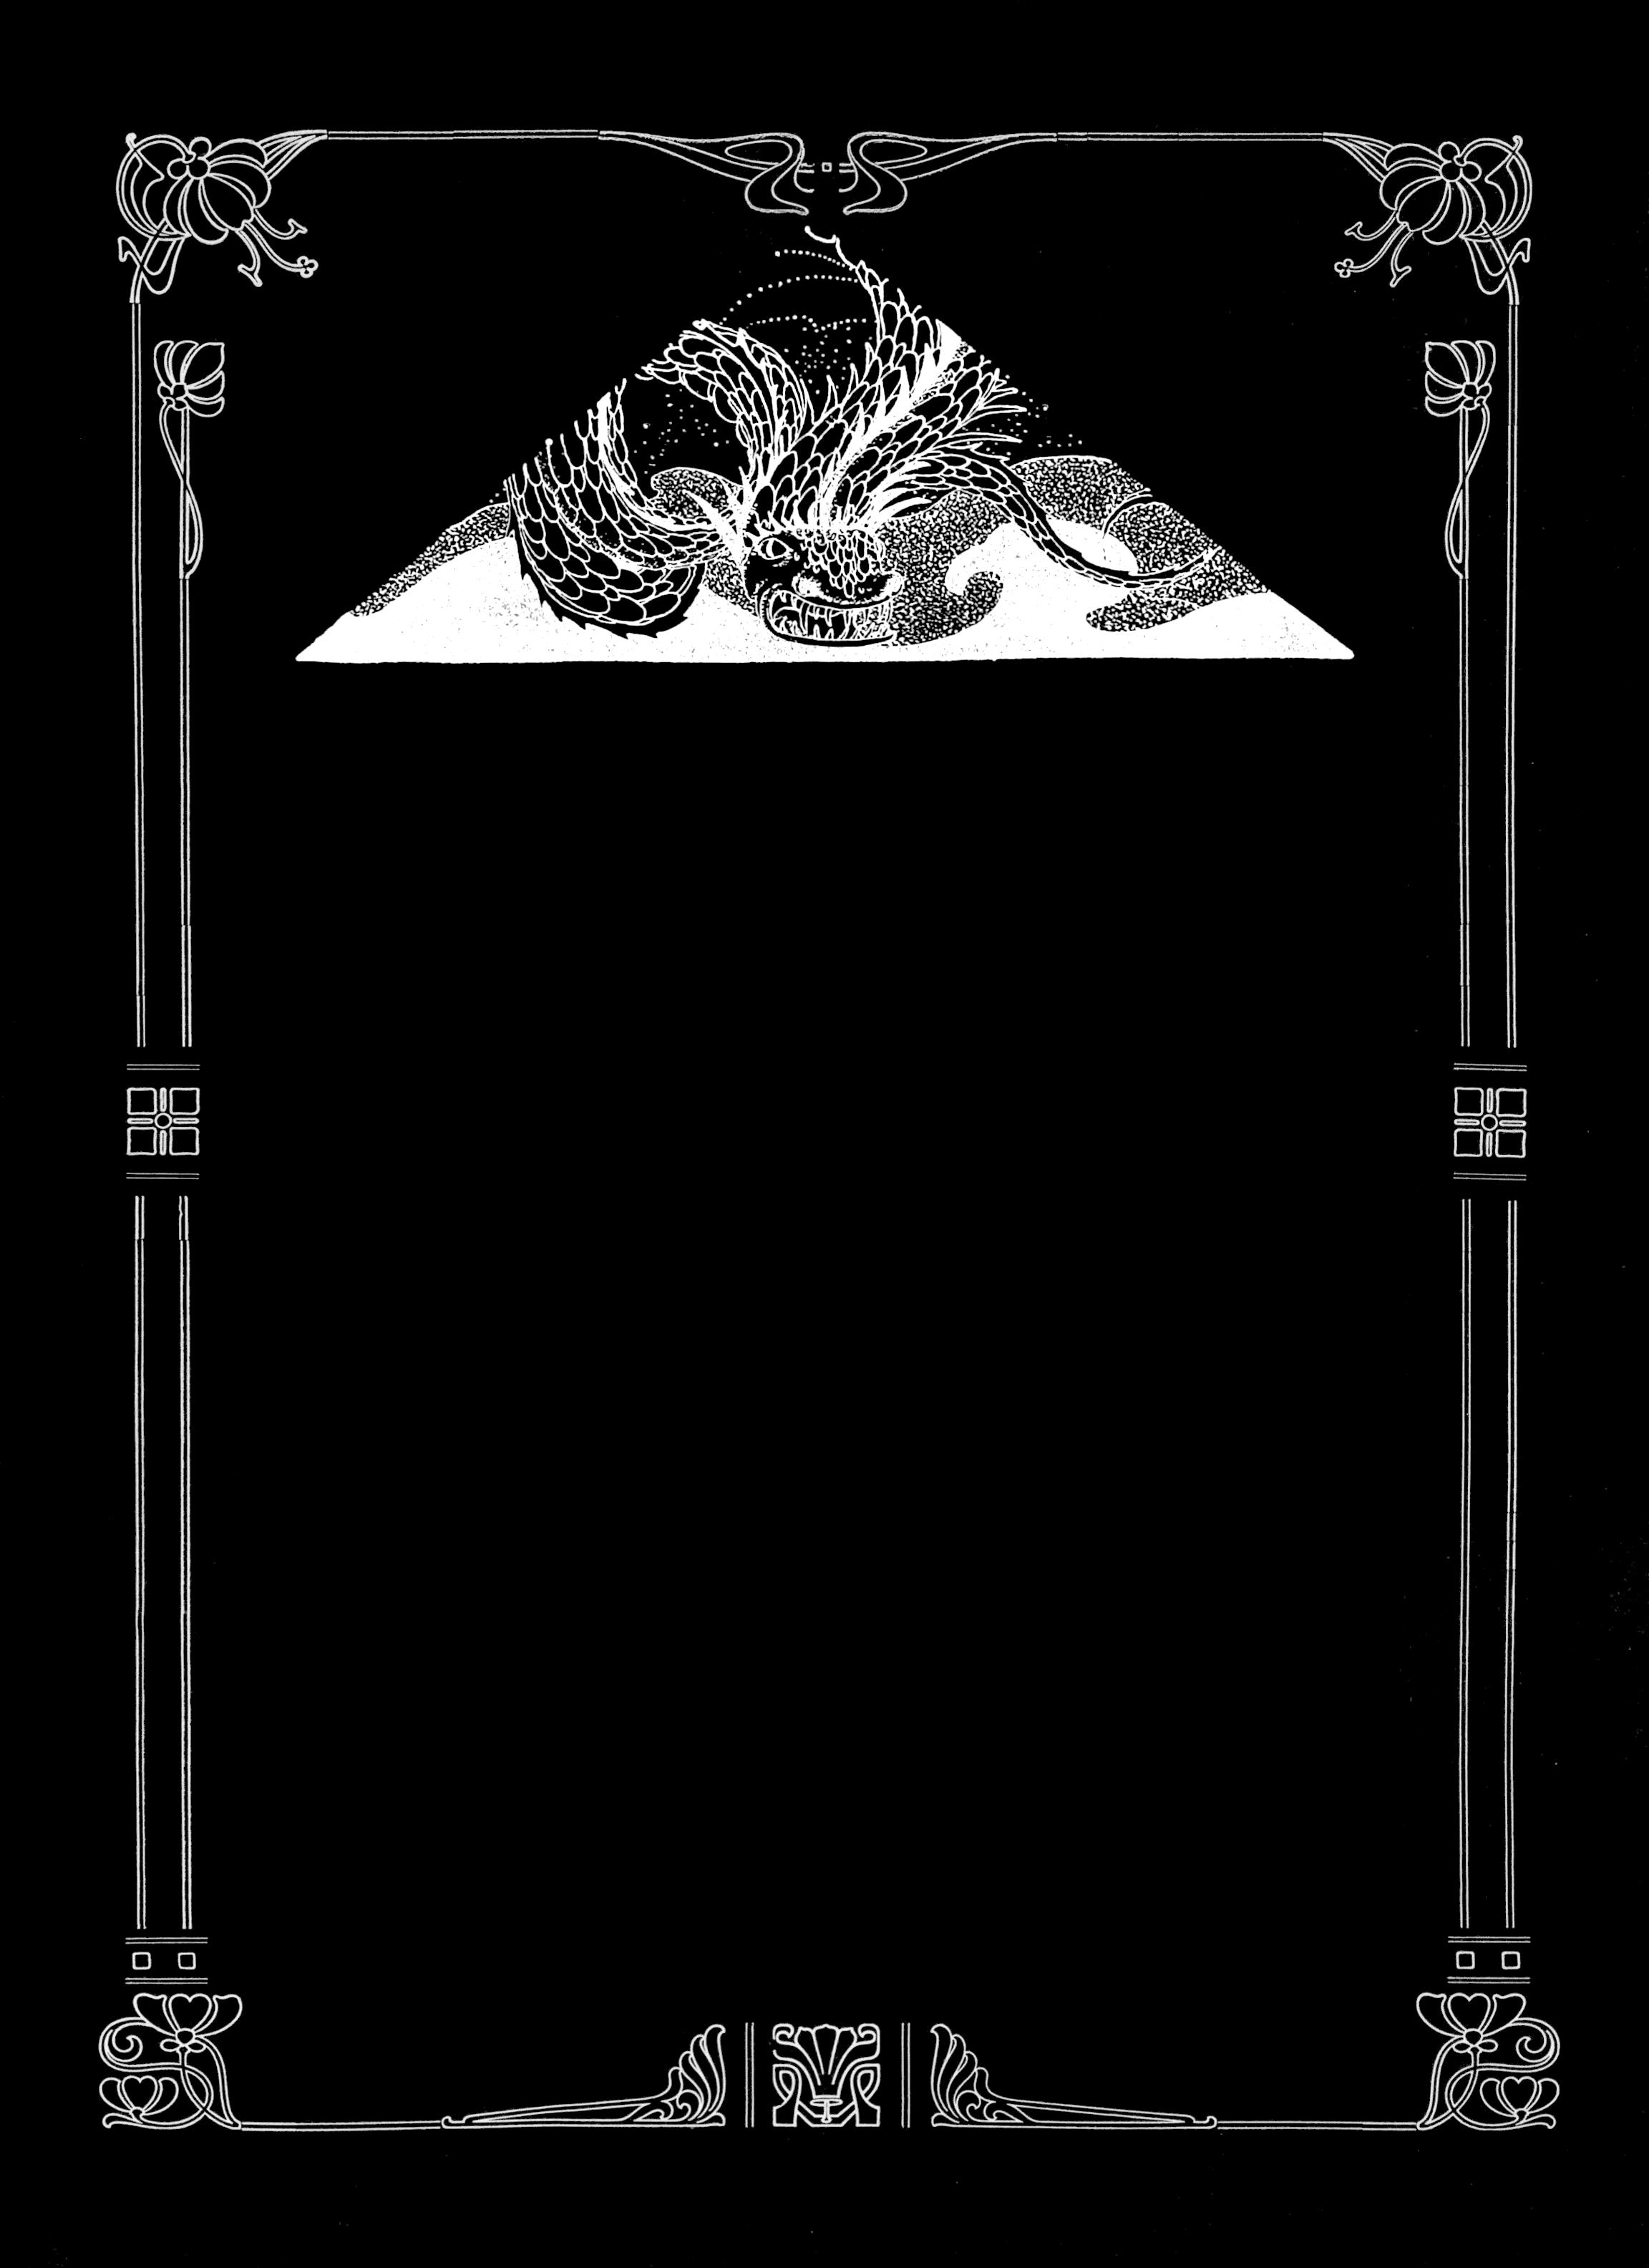
\includegraphics[width=\paperwidth,height=\paperheight]{dragon-blackandwhite.png}}
\pagenumbering{gobble}
\begin{document}
\vspace*{\fill}
\Huge
\begin{center}
夢溪筆談
\end{center}
\bigskip
\begin{center}
沈括
\end{center}
\vspace*{\fill}
\clearpage
\normalsize
\tableofcontents
\clearpage
\Large
\pagenumbering{arabic}
\section{卷一 故事一}
\paragraph{}
上親郊郊廟,冊文皆曰``恭荐歲事''。先景靈宮,謂之``朝獻'';次太 廟,謂之``朝饗'';末乃有事于南郊。予集《郊式》時,曾預討論,常疑其 次序,若先為尊,則效不應在廟后;若后為尊,則景靈宮不應在太廟之先。 求共所從來,蓋有所因。按唐故事,凡有事地上帝,則百神皆預遣使祭告, 唯太清宮、太廟則皇帝親行。其冊祝皆曰``取某月某日有事于某所,不敢不 告。''宮、廟謂之``奏告'',余皆謂之``祭告''。唯有事于南郊,方為``正 祠''。至天寶九載,乃下詔曰:```告 '者,上告下之詞。今后太清宮宜稱 `朝獻',太廟稱`朝饗'。''自此遂失``奏告''之名,冊文皆為``正祠''。   正衙法座,香木為之,加金飾,四足,墮角,其前小偃,織藤冒之。每車 駕出幸,則使老內臣馬上抱之,曰``駕頭''。輦后曲蓋謂之``筤''。兩扇夾心 ,通謂之``扇筤''。皆繡,亦有銷金者,即古之華蓋也。   唐翰林院在禁中,乃人主燕居之所,玉堂、承明、金鑾殿皆在其間。應供 奉之人,自學士已下,工伎群官司隸籍其間者,皆稱翰林,如今之翰林醫官、 翰林待詔之類是也。唯翰林茶酒司止稱``翰林司'',蓋相承闕文。唐制,自宰 相而下,初命皆無宣召之禮,惟學士宣召。蓋學士院在禁中,非內臣宣召,無 因得入,故院門別設復門,亦以其通禁庭也。又學士院北扉者,為其在浴堂之 南,便于應召。今學士初拜,自東華門入,至左承天門下馬;待詔、院吏自左 承天門雙引至秃門。此亦用唐故事也。唐宣召學士,自東門入者,彼時學士院 在西掖,故自翰林院東門赴召,非若今之東華門也。至如挽鈴故事,亦緣其在 禁中,雖學士院吏,亦止于玉堂門外,則其嚴密可知。如今學士院在外,与諸 司無异,亦設鈴索,悉皆文具故事而已。   學士院玉堂,太宗皇帝曾親幸。至今唯學士上日許正坐,他日皆不敢獨坐 。故事:堂中設視草台,每草制,則具衣冠据台而坐。今不復如此,但存空台 而已。玉堂東承旨秃子窗格上有火然處。太宗嘗夜幸玉堂,蘇易簡為學士,已 寢,遽起,無燭具衣冠,宮嬪自窗格引燭入照之。至今不欲更易,以為玉堂一 盛事。   東西頭供奉官,本唐從官之名。自永微以后,人主多居大明宮,別置從官 ,謂之``東頭供奉官''。西內具員不廢,則謂之``西頭供奉官''。   唐制,兩省供奉官東西對立,謂之``蛾眉班''。國初,供奉班于百官前橫 列。王溥罷相為東宮,一品班在供奉班之后,遂令供奉班依舊分立。慶歷賈安 公為中丞,以東西班對拜為非禮,復令橫行。至今初敘班分立;百官班定,乃 轉班橫行;參罷,復分立;百官班退,乃出。參用舊制也。   衣冠故事,多無著令,但相承為例;如學士舍人躡履見丞相,往還用平狀 ,扣階乘馬之類,皆用故事也。近歲多用靴簡。章子厚為學士日,因事論列, 今則遂為著令矣。   中國衣冠,自北齊以來,乃全用胡服。窄袖、緋綠短衣、長靿靴、有鞢 帶,皆胡服也。窄袖利于馳射,短衣、長靿皆便于涉草。胡人樂茂草,常寢處 其間,予使北時皆見之。雖王庭亦在深荐中。予至胡庭日,新雨過,涉草,衣 褲皆濡,唯胡人都無所沾。帶衣所垂蹀躞,蓋欲佩帶弓劍、□帨、算囊、刀礪 之類。自后雖去蹀躞,而猶存其環,環所以銜蹀躞,如馬之□根,即今之帶銙 也。天子必以十三環為節,唐武德貞觀時猶爾。開元之后,雖仍舊俗,而稍褒 博矣。然帶鉤尚穿帶本為孔,本朝加順折,茂人文也。帕頭一謂之四腳,乃四 帶也。二帶系腦后垂之,二帶反系頭上,令曲折附頂,故亦謂之``折上巾''。 唐制,唯人主得用硬腳。晚唐方鎮擅命,始僭用硬腳。本朝帕頭有直腳、局腳 、交腳、朝天、順風,凡五等。唯直腳貴賤通服之。又庶人所戴頭巾,唐人亦 謂之``四腳'',蓋兩腳系腦后,兩腳系頷下,取其服勞不脫也。無事則反系于 頂上。今人不復系頷下,兩帶遂為虛設。   唐中書指揮事謂之``堂帖子'',曾見唐人堂帖,宰相簽押,格如今之堂劄 子也。   予及史館檢討時,議樞密院劄子問宣頭所起。余按唐故事,中書舍人職堂 語詔,皆寫四本:一本為底,一本為宣。此``宣''謂行出耳,未以名書也。晚 唐樞密使自禁中受旨,出付中書,即謂之``宣''。中書承受,錄之于籍,謂之 ``宣底''。今史館中尚有故《宣底》二卷,如今之《圣語簿》也。梁朝初置崇 仁院,專行密命。至后唐庄宗復樞密使,使郭崇韜、安重誨為之,始分領政事 ,不關由中書直行下者謂之``宣'',如中書之``敕''。小事則發頭子,擬堂貼 也。至今樞密院用宣及頭子,本朝樞密院亦用劄子。但中書劄子,宰相押字在 上,次相及參政以次向下;樞密院劄子,樞長押字在下,副貳以次向上:以此 為別。頭子唯給驛馬之類用之。   百官于中書見宰相,九卿而下,即省吏高聲唱一聲``屈'',則趨而入。宰 相揖及進茶,皆抗聲贊喝,謂之``屈揖''。待制以上見,則言``請某官'',更 不屈揖,臨退仍進湯,皆于席南橫設百官之位,升朝則坐,京官已下皆立。后 殿引臣寮,則待制已上宣名拜舞;庶官但贊拜,不宣名,不舞蹈。中書略貴者 ,示与之抗也。上前則略微者,殺禮也。   唐制,丞郎拜官,即籠門謝。今三司副使已上拜官,則拜舞于子階上;百 官拜于階下,而不舞蹈。此亦籠門故事也。   學士院第三廳學士秃子,當前有一巨槐,素號``槐廳''。舊傳居此秃者, 多至入相。學士爭槐廳,至有抵徹前人行李而強据之者。余為學士時,目觀此 事。   諫議班在知制誥上;若帶待制,則在知制誥下,從職也,戲語謂之``帶墜 ''。   《集賢院記》:``開元故事,校書官許稱學士''。今三館職事,皆稱``學 士'',用開元故事也。   館閣新書淨本有誤書處,以雌黃涂之。嘗校改字之法:刮洗則傷紙,紙貼 之又易脫,粉涂則字不沒,涂數遍方能漫滅。唯雌黃一漫則滅,仍久而不脫。 古人謂之鉛黃,蓋用之有素矣。   余為鄜延經略使日,新一廳,謂之五司廳。延州正廳乃都督廳,治延州事 ;五司廳治鄜延路軍事,如唐之使院也。五司者,經略、安撫、總管、節度、 觀察也。唐制、方鎮綿帶節度、觀察、處置三使。今節度之職,多歸總管司; 觀察歸安撫司;處置歸經略司。其節度、觀察兩案,并支掌推官、判官,今皆 治州事而已。經略、安撫司不置佐官,以帥權不可更不專也。都總管、副總管 、鈐轄、都監同簽書,而皆受經略使節制。   銀台司兼門下封駁,乃給事中之職,當隸門下省,故事乃隸樞密院。下寺 監皆行劄子;寺監具申狀,雖三司,亦言``上銀台''。主判不以官品,初冬獨 賜翠毛錦袍。學士以上,自從本品。行案用樞密院雜司人吏,主判食樞密廚, 蓋樞密院子司也。   大駕鹵簿中有勘箭,如古之勘契也。其牡謂之``雄牡箭'',牝謂之``辟仗 箭''。本胡法也。熙宁中罷之。   前世藏書,分隸數處,蓋防水火散亡也。今三館、秘閣,凡四處藏書,然 同在崇文院。其間官書,多為人盜竊,士大夫家往往得之。嘉祐中,置編校官 八員,雜讎四館書。給吏百人,悉以黃紙為大冊寫之。自此私家不敢輒藏。校 讎累年,僅能終昭文一館之書而罷。   舊翰林學士地勢清切,皆不兼他務。文館職任,自校理以上,皆有職錢, 唯內外制不給。楊大年久為學士,家貧,請外,表詞千余言,其間兩聯曰:`` 虛忝甘泉之從臣,終作莫敖之餒鬼。''``從者之病莫興,方朔之饑欲死。''京 師百官上日,唯翰林學士敕設用樂,他雖宰相,亦無此禮。优伶并開封府點集 。陳和叔除學士時,和叔知開封府,遂不用女优。學士院敕設不用女优,自和 叔始。   禮部貢院試進士日,設香案于階前,主司与舉人對拜,此唐故事也。所坐 設位供張甚盛,有司具茶湯飲漿。至試學究,則悉徹帳幕氈席之類,亦無茶湯 ,渴則飲硯水,人人皆黔其吻。非故欲困之,乃防氈幕及供應人私傳所試經義 。蓋嘗有敗者,故事為之防。歐文忠有詩:``焚香禮進士,徹幕待經生。''以 為禮數重輕如此,其實自有謂也。   嘉祐中,進士奏名訖,未御試,京師妄傳``王俊民為狀元'',不知言之所 起,人亦莫知俊民為何人。及御試,王荊公時為知制誥,与天章閣待制楊樂道 二人為詳定官。舊制,御試舉人,設初考官,先定等第;復彌之以送覆考官, 再定等第;乃付詳定官,發初考官所定等,以對覆考之等:如同即已;不同, 則詳其程文,當從初考或從覆考為定,即不得別立等。是時,王荊公以初、覆 考所定第一人皆未允當,于行間別取一人為狀首。楊樂道守法,以為不可。議 論未決,太常少卿朱從道時為封彌官,聞之,謂同舍曰:``二公何用力爭,從 道十日前已聞王俊民為狀元,事必前定。二公恨自苦耳。''既而二人各以已意 進稟,而詔從荊公之請。及發封,乃王俊民也。詳定官得別立等,自此始,遂 為定制。   選人不得乘馬入宮門。天圣中,選人為館職,始歐陽永叔、黃鑒輩,皆自 左掖門下馬入館,當時謂之``步行學士''。嘉祐中,于崇文院置編校局,校官 皆許乘馬至院門。其后中書五房置習學公事官,亦緣例乘馬赴局。   車駕行境,前驅謂之隊,則古之清道也。其次衛仗,衛仗者,視闌入宮門 法,則古之外仗也。其中謂之禁圍,如殿中仗。《天官》:``掌舍,無宮,則 供人門。''今謂之``殿門天武官'',极天下長人之選八人。上御前殿,則執鉞 立于紫宸門下;行幸則為禁圍門,行于仗馬之前。又有衡門十人,隊長一人, 選諸武力絕倫者為之。上御后殿,則執檛東西對立于殿前,亦古之虎賁、人門 之類也。   余嘗購得后唐閔帝應順元年案檢一通,乃除宰相劉昫兼判三絲堂檢。前有 擬狀云:``具官劉昫。右,伏以劉昫經國才高,正君志切,方屬体元之運,實 資謀始之規。宜注宸衷,委司判計,漸期富庶,永贊圣明。臣等商量,望授依 前中書侍郎,兼吏部尚書、同中書門下平章事,充集賢殿大學士,兼判三司, 散官勳封如故,未審可否?如蒙允許,望付翰林降制處分,謹錄奏聞。''其后 有制書曰:``宰臣劉昫,右,可兼判三司公事,宜令中書門下依此施行。付中 書門下,準此。四月十日。''用御前新鑄之印。与今政府行遣稍异。   本朝要事對稟,常事擬進入,畫可然后施行,謂之``熟狀''。事速不及待 報,則先行下,具制草奏知,謂之``進草''。熟狀白紙書,宰相押字,他執政 具姓名。進草即黃紙書,宰臣、執政皆于狀背押字。堂檢,宰、執皆不押,唯 宰屬于檢背書日,堂吏書名用印。此擬狀有詞,宰相押檢不印,此其為异也。 大率唐人風俗,自朝廷下至郡縣,決事皆有詞,謂之判,則書判科是也。押檢 二人,乃馮道、李愚也。狀檢瀛王親筆,甚有改竄勾抹處。按《舊五代史》: ``應順元年四月九日已卯,鄂王薨。庚辰,以宰相劉昫判三司。''正是十日, 与此檢無差。宋次道記《開元宰相奏請》、鄭畋《鳳池稿草》、《擬狀注制集 》悉多用四六,皆宰相自草。今此擬狀,馮道親筆,蓋故事也。   舊制,中書、樞密院、三司使印并涂金。近制,三省、樞密院印用銀為之 ,涂金;余皆鑄銅而已。
\clearpage
\section{卷二 故事二}
\paragraph{}
三司使班在翰林學士之上。舊制,權使即与正同,故三司使結銜皆在官職 之上。慶歷中,葉道卿為權三司使,執政有欲抑道卿者,降敕時移權三司使在 職下結銜,遂立翰林學士之下,至今為例。后嘗有人論列,結銜雖依舊,而權 三司使初除,秃門取旨,間有敘學士者,然不為定制。   宗子授南班官,世傳王文正太尉為宰相日,始開此議,不然也。故事,宗 子無遷官法,唯遇稀曠大慶,則普遷一官。景祐中,初定祖宗并配南郊,宗室 欲緣大禮乞推恩,使諸王宮教授刁約草表上聞。后約見丞相王沂公,公問:`` 前日宗室乞遷官表,何人所為?''約未測其意,答以不知。歸而思之,恐事窮 且得罪,乃再詣相府。沂公問之如前,約愈恐,不復敢隱,遂以實對。公曰: ``無他,但愛其文詞耳。''再三嘉獎。徐曰:``已得旨,別有措置。更數日, 當有指揮。''自此遂有南班之授,近屬自初除小將軍,凡七遷則為節度使,遂 為定制。諸宗子以千縑謝約,約辭不敢受。余与刁親舊,刁嘗出表稿以示余。   大理法官,皆親節案,不得使吏人。中書檢正官不置吏人,每房給楷書一 人錄淨而已。蓋欲士人躬親職事,格吏奸,兼歷試人才也。   太宗命創方團球帶,賜二府文臣。其后樞密使兼侍中張耆、王貽永皆特賜 ;李用和、曹郡王皆以元舅賜;近歲宣微使王君貺以耆舊特賜。皆出异數,非 例也。近歲京師士人朝服乘馬,以黲衣蒙之,謂之``涼衫'',亦古之遺法也。 《儀禮》``朝服加景''是也。但不知古人制度章色如何耳。   內外制凡草制除官,自給諫、待制以上,皆有潤筆物。太宗時,立潤筆錢 數,降詔刻石于舍人院。每除官,則移文督之。在院官下至吏人院騶,皆分沾 。元丰中,改立官制,內外制皆有添給,罷潤筆之物。   唐制,官序未至而以他官權攝者,為直官,如許敬宗為直記室是也。國朝 學士、舍人皆置直院。熙宁中,復置直舍人、學士院,但以資淺者為之,其實 正官也。熙宁六年,舍人皆遷罷,閣下無人,乃以章子平權知制誥,而不除直 院者,以其暫攝也。古之兼官,多是暫時攝領;有長兼者,即同正官。余家藏 《海陵王墓志》謝朓文,稱``兼中書侍郎。''   三司、開封府、外州長官升廳事,則有衙吏前導告喝。國朝之制,在禁中 唯三官得告:宰相告于中書,翰林學士告于本院,御史告于朝堂。皆用朱衣吏 ,謂之``三告官''。所經過處,閽吏以梃扣地警眾,謂之``打仗子''。兩府、 親王,自殿門打至本司及上馬處;宣微使打于本院;三司使、知開封府打于本 司。近歲寺監長官亦打,非故事。前宰相赴朝,亦有特旨,許張蓋、打仗子者 ,系臨時指揮。執絲梢鞭入內,自三司副使以上;副使唯乘紫絲暖座從入。隊 長持破木梃,自待制以上。近歲寺監長官持藤杖,非故事也。百官儀范,著令 之外,諸家所記,尚有遺者。雖至猥細,亦一時儀物也。   國朝未改官制以前,异姓未有兼中書令者,唯贈官方有之。元丰中,曹郡 王以元舅特除兼中書令,下度支給俸。有司言:``自來未有活中書令請受則例 。''   都堂及寺觀百官會集坐次,多出臨時。唐以前故事,皆不可考,唯顏真卿 与左仆射定襄郡子王郭英又書云:``宰相、御史大夫、兩省五品、供奉官自為 一行,十二衛大將軍次之,三師、三公、令仆、少師、保傅、尚書左右丞、侍 郎自為一行,九卿、三監對之。從古以來,未嘗參錯。''此亦略見當時故事, 今錄于此,以備闕文。   賜``功臣''號,始于唐德宗奉天之役。自后藩鎮,下至從軍資深者,例賜 ``功臣''。本朝唯以賜將相。熙宁中,因上皇帝尊號,宰相率同列面請三四, 上終不允,曰:``徽號正如卿等`功臣',何補名實?''是時吳正憲為首相, 乃請止``功臣''號,從之。自是群臣相繼請罷,遂不復賜。
\clearpage
\section{卷三 辨證一}
\paragraph{}
鈞石之石,五權之名,石重百二十斤。后人以一斛為一石,自漢已如此 ,``飲酒一石不亂''是也。挽蹶弓弩,古人以鈞石率之。今人乃以粳米一斛 之重為一石。凡石者,以九十二斤半為法,乃漢秤三百四十一斤也。今之武 卒蹶弩,有及九石者,計其力乃古之二十五石,比魏之武卒,人當二人有余 ;弓有挽三石者,乃古之三十四鈞,比顏高之弓,人當五人有余。此皆近歲 教養所成。以至擊刺馳射,皆盡夷夏之術;器仗鎧胄,极今古之工巧。武備 之盛,前世未有其比。

《楚詞·招魂》尾句皆曰``些'',蘇個反。今夔、峽、湖、湘及南、北 江獠人,凡禁咒句尾皆稱``些''。此乃楚人舊俗,即梵語``薩最訶''也。薩 音桑葛反,最無可反,訶從去聲。三字合言之,即``些''字也。

陽燧照物皆倒,中間有礙故也。算家謂之``格術''。如人搖櫓,臬為之 礙故也。若鳶飛空中,其影隨鳶而移,或中間為窗隙所束,則影与鳶遂相違 ,鳶東則影西,鳶西則影東。又如窗隙中樓塔之影,中間為窗所束,亦皆倒 垂,与陽燧一也。陽燧面洼,以一指迫而照之則正;漸遠則無所見;過此遂 倒。其無所見處,正如窗隙、櫓臬、腰鼓礙之,本末相格,遂成搖櫓之勢。 故舉手則影愈下,下手則影愈上,此其可見。陽燧面洼,向日照之,光皆聚 向內。离鏡一、二寸,光聚為一點,大如麻菽,著物則火發,此則腰鼓最細 處也。豈特物為然,人亦如是,中間不為物礙者鮮矣。小則利害相易,是非 相反;大則以已為物,以物為已。不求去礙,而欲見不顛倒,難矣哉!《酉 陽雜俎》謂``海翻則塔影倒'',此妄說也。影入窗隙則倒,乃其常理。

先儒以日食正陽之月止謂四月,不然也。正、陽乃兩事,正謂四月,陽 謂十月。日月陽止是也。《詩》有``正月繁霜'';``十月之交,朔月辛卯。 日有食之,亦孔之丑''二者,此先王所惡也。蓋四月純陽,不欲為陰所侵; 十月純陰,不欲過而干陽也。

余為《喪服后傳》,書成,熙宁中欲重定五服敕,而余預討論。雷、鄭 之前,闕謬固多,其間高祖遠孫一事,尤為無義。《喪服》但有曾祖齊衰六 月,遠曾緦麻三月,而無高祖遠孫服。先儒皆以謂``服同曾祖曾孫,故不言 可推而知'',或曰``經之所不言則不服'',皆不然也。曾,重也。由祖而上 者,皆曾祖也;由孫而下者,皆曾孫也:雖百世可也。苟有相逮者,則必為 服喪三月。故雖成王之于后稷,亦稱曾孫。而祭禮祝文,無遠近皆曰曾孫。 《禮》所謂``以五為九''者,謂傍親之殺也。上殺、下殺至于九,傍殺至于 四,而皆謂之族。族昆弟父母、族祖父母、族曾祖父母。過此則非其族也。 非其族,則為之無服。唯正統不以族名,則是無絕道也。

舊傳黃陵二女,堯子舜妃。以二帝化道之盛,始于閨房,則二女當具任 、姒之德。考其年歲,帝舜陟方之時,二妃之齒已百歲矣。后人詩騷所賦, 皆以女子待之,語多瀆慢,皆禮義之罪人也。

歷代官室中有謻門,蓋取張衡《東京賦》``謻門曲榭''也。說者謂``冰 室門''。按《字訓》:``謻,別也。''《東京賦》但言別門耳,故以對曲榭 ,非有定處也。

水以漳名、洛名者最多,今略舉數處:趙、晉之間有清漳、濁漳,當陽 有漳水,灨上有漳水,鄣郡有漳江,漳州有漳浦,亳州有漳水,安州有漳水 。洛中有洛水,北地郡有洛水,沙縣有洛水。此概舉一二耳,其詳不能具載 。余考其義,乃清濁相蹂者為漳。章者,文也,別也。漳謂兩物相合,有文 章,且可別也。清漳、濁漳,合于上党。當陽即沮、漳合流,贛上即漳、灨 合流,漳州余未曾目見,鄣郡即西江合流,亳、漳則漳、渦合流,云夢則漳 、鄖合流。此數處皆清濁合流,色理如螮蝀,數十里方混。如璋亦從章,璋 ,王之左右之臣所執,《詩》云:``濟濟辟王,左右趣之。濟濟辟王,左右 奉璋。''璋,圭之半体也。合之則成圭。王左右之臣,合体一心,趣乎王者 也。又諸侯以聘女,取其判合也。有事于山川,以其殺宗廟禮之半也。又牙 璋以起軍旅,先儒謂``有鉏牙之飾于剡側'',不然也。牙璋,判合之器也, 當于合處為牙,如今之合契。牙璋,牡契也,以起軍旅,則其牝宜在軍中, 即虎符之法也。洛与落同義,謂水自上而下,有投流處。今淝水、沱水,天 下亦多,先儒皆自有解。

解州鹽澤,方百二十里。久雨,四山之水悉注其中,未嘗溢;大旱未嘗 涸。鹵色正赤,在版泉之下,俚俗謂之``蚩尤血''。唯中間有一泉,乃是甘 泉,得此水然后可以聚人。其北有堯梢音消水,一謂之巫咸河。大鹵之水, 不得甘泉和之,不能成鹽。唯巫咸水入,則鹽不復結,故人謂之``無咸河'' ,為鹽澤之患,筑大堤以防之,甚于備寇盜。原其理,蓋巫咸乃濁水,入鹵 中,則淤淀鹵脈,鹽遂不成,非有他异也。

《庄子》云:``程生馬。''嘗觀《文字注》:``秦人謂豹曰程。''余至 延州,人至今謂虎豹為``程'',蓋言``虫''也。方言如此,抑亦舊俗也。

《唐六典》述五行,有祿命、驛馬、湴河之目。人多不曉湴河之義。余 在鄜延,見安南行營諸將閱兵馬藉,有稱``過范河損失''。問其何謂``范何 ''?乃越人謂淖沙為``范河'',北人謂之``活沙''。余嘗過無定河,度活沙 ,人馬履之,百步之外皆動,澒澒然如人行幕上。其下足處雖甚堅,若遇其 一陷,則人馬蹻車,應時皆沒,至有數百人平陷無孑遺者。或謂:此即流沙 也。又謂:沙隨風流,謂之流沙。湴,字書亦作``泥''。蒲濫反。按古文, 泥,深泥也。本書有湴河者,蓋謂陷運,如今之``空亡''也。

古人藏書辟蠹用芸。芸,香草也,今人謂之七里香者是也。葉類豌豆, 作小叢生,其葉极芬香,秋間葉間微白如粉污,辟蠹殊驗。南人采置席下, 能去蚤虱。余判昭文館時,曾得數株于潞公家,移植秘閣后,今不復有存者 。香草之類,大率多异名,所謂蘭蓀,蓀,即今菖蒲是也;蕙,今零陵香是 也;茞,今白芷是也。

祭禮有腥、燖、熟三獻。舊說以謂腥、燖備太古、中古之禮,余以為不 然。先王之于死者,以為之無知則不仁,以之為有知則不智。荐可食之熟, 所以為仁;不可食之腥、燖,所以為智。又一說,腥、燖以鬼道接之,饋食 以人道接之,致疑也。或謂鬼神嗜腥、燖,此雖出于异說,圣人知鬼神之情 狀,或有此理,未可致詰。

世以玄為淺黑色,璊為赭玉,皆不然也。玄乃赤黑色,燕羽是也,故謂 之玄鳥。熙宁中,京師貴人戚里,多衣深紫色。謂之黑紫,与皂相亂,几不 可分,乃所謂玄也。璊。赭色也。``毳衣如璊'';音門。稷之璊色者謂之穈 。穈字音門,以其色命之也。《詩》:``有穈有芑。''今秦人音糜,聲之訛 也。穈色在朱黃之間,似乎赭,极光瑩,掬之粲,澤熠熠如赤珠。此自是一 色,似赭非赭。蓋所謂璊,色名也,而從玉,以其赭而澤,故以諭之也。猶 鴘以色名而從鳥,以鳥色諭之也。

世間鍛鐵所謂鋼鐵者,用柔鐵屈盤之,乃以生鐵陷其間,泥封煉之,鍛 令相入,謂之``團鋼'',亦謂之``灌鋼''。此乃偽鋼耳,暫假生鐵以為堅, 二三煉則生鐵自熟,仍是柔鐵。然而天下莫以為非者,蓋未識真鋼耳。余出 使,至磁州鍛坊,觀煉鐵,方識真鋼。凡鐵之有鋼者,如面中有筋,濯盡柔 面,則面筋乃見。煉鋼亦然,但取精鐵,鍛之百余火,每鍛稱之,一鍛一輕 ,至累鍛而斤兩不減,則純鋼也,雖百煉不耗矣。此乃鐵之精純者,其色清 明,磨瑩之,則黯黯然青且黑,与常鐵迥异。亦有煉之至盡而全無鋼者,皆 系地之所產。

《詩》:``芄蘭之支,童子佩觿。''觿,解結錐也。芄蘭生莢支,出于 葉間,垂之正如解結錐。所謂``佩觿''者,疑古人為韘之制,亦當与芄蘭之 葉相似,但今不復見耳。

江南有小栗,謂之``茅栗''。茅音草茅之茅。以余觀之,此正所謂芧也 。則《庄子》所謂``狙公賦芧''者,芧音序。此文相近之誤也。

余家有閻博陵畫唐秦府十八學士,各有真贊,亦唐人書,多与舊史不同 :姚柬字思廉,舊史乃姚思廉字簡之。蘇台、陸元朗、薛庄,《唐書》皆以 字為名。李玄道、蓋文達、于志宁、許敬宗、劉教孫、蔡允恭,《唐書》皆 不書字。房玄齡字喬年,《唐書》乃房喬字玄齡。孔穎達字穎達,《唐書》 字仲達。蘇典簽名旭,《唐書》乃勖。許敬宗、薛庄官皆直記室,《唐書》 乃攝記室。蓋《唐書》成于后人之手,所傳容有訛謬;此乃當時所記也。以 舊史考之,魏鄭公對太宗云:`` 目如懸鈴者佳。''則玄齡果名,非字也。 然蘇世長,太宗召對玄武門,問云:``卿何名長意短?''后乃為學士,似為 學士時,方更名耳。

唐貞觀中,敕下度支求杜若,省郎以謝朓詩云:``芳洲采杜若。''乃責 坊州貢之。當時以為嗤笑。至如唐故事,中書省中植紫薇花,何异坊州貢杜 若,然歷世循之,不以為非。至今舍人院紫微閣前植紫薇花,用唐故事也。

漢人有飲酒一石不亂。余以制酒法較之,每粗米二斛,釀成酒六斛六斗 。今酒之至醨者,每秫一斛,不過成酒一斛五斗,若如漢法,則粗有酒气而 已。能飲者飲多不亂,宜無足怪。然漢之一斛,亦是今之二斗七升。人之腹 中,亦何容置二斗七升水邪?或謂:``石乃鈞石之石,百二十斤。''以今秤 計之,當三十二斤,亦今之三斗酒也。于定國食酒數石不亂,疑無此理。

古說濟水伏流地中,今歷下凡發地皆是流水,世傳濟水經過其下。東阿 亦濟水所經,取井水煮膠,謂之``阿膠'';用攪濁水則清。人服之,下膈、 疏痰、止吐,皆取濟水性趨下清而重,故以治淤濁及逆上之疾。今醫方不載 此意。

余見人為文章多言``前榮'',榮者,夏屋東西序之外屋翼也,謂之東榮 、西榮。四注屋則謂之東霤、西霤。未知前榮安在?

宗廟之祭西向者,室中之祭也。藏主于西壁,以其生者之處奧也。即主 祏而求之,所以西向而祭。至三獻則尸出于室,坐于戶西南面,此堂上之祭 也。戶西謂扆,設扆于此。左戶、右牖,戶、牖之間謂之扆。坐于戶西,即 當扆而坐也。上堂設位而亦東向者,設用室中之禮也。

``人而不為《周南》、《召南》,其猶正牆面而立也。''《周南》、《 召南》樂名也。``胥鼓《南》'';``以《雅》以《南》''是也。《關雎》、 《鵲巢》,二《南》之詩,而已有樂有舞焉。學者之事,其始也學《周南》 、《召南》,末至于舞《大夏》、《大武》。所謂為《周南》、《召南》者 ,不獨誦其詩而已。

《庄子》言:``野馬也,塵埃也。''乃是兩物。古人即謂野馬為塵埃, 如吳融云:``動梁間之野馬。''又韓偓云:``窗里日光飛野馬。''皆以塵為 野馬,恐不然也。野馬乃田野間浮气耳,遠望如群馬,又如水波,佛書謂`` 如熱時野馬陽焰'',即此物也。

蒲蘆,說者以為蜾贏,疑不然。蒲蘆,即蒲、葦耳。故曰:``人道敏政 ,地道敏藝''。夫政猶蒲蘆也,人之為政,猶地之藝蒲葦,遂之而已,亦行 其所無事也。

余考樂律,及受詔改鑄渾儀,求秦漢以前度量斗升:計六斗當今一斗七 升九合;秤三斤當今十三兩;一斤當今四兩三分兩之一,一兩當今六銖半。 為升中方;古尺二寸五分十分分之三,今尺一寸八分百分分之四十五強。

十神太一:一曰太一,次曰五福太一,三曰天一太一,四曰地太一,五 曰君基太一,六曰臣基太一,七曰民基太一,八曰大游太一,九曰九气太一 ,十曰十神太一。唯太一最尊,更無別名,止謂之太一。三年一移。后人以 其別無名,遂對大游而謂之小游太一,此出于后人誤加之。京師東西太一宮 ,正殿祠五福,而太一乃在廊廡,甚為失序。熙宁中,初營中太一宮,下太 史考定神位。余時領太史,預其議論。今前殿祠五福,而太一別為后殿,各 全其尊,深為得禮。然君基、臣基、民基,避唐明帝諱改為``棋'',至今仍 襲舊名,未曾改正。

余嘉祐中客宣州宁國縣,縣人有方璵者,其高祖方虔,為楊行密守將, 總兵戍宁國,以備兩浙。虔后為吳人所擒,其子從訓代守宁國,故子孫至今 為宁國人。有楊溥与方虔、方從訓手教數十紙,紙扎皆精善。教稱委曲書 ,押處稱``使'',或稱``吳王''。內一紙報方虔云:``錢鏐此月內已亡歿'' 。紙尾書``正月二十九日。''按《五代史》,錢鏐以后唐長興二年卒,楊溥 天成四年已僭即偽位,豈得長興二年尚稱``吳王''?溥手教所指揮事甚詳, 翰墨印記,极有次序,悉是當時親跡。今按,天成四年歲庚寅,長興三年歲 壬辰,計差二年。溥手教,余得其四紙,至今家藏。
\clearpage
\section{卷四 辨證二}
\paragraph{}
司馬相如《上林賦》敘上林諸水曰:丹水,紫淵,灞、滻、涇、謂,`` 八川分流,相背而异態'',``灝溔潢漾……東注太湖。''八川自入大河,大 河去太湖數千里,中間隔太山及淮、濟、大江,何緣与太湖相涉?郭璞《江 賦》云:``注五湖以漫漭,灌三江而漰沛。''《墨子》曰:``禹治天下,南 為江、漢、淮、汝,東流注之五湖。''孔安國曰:``自彭蠡,江分為三,入 于震澤后,為北江而入于海。''此皆未嘗詳考地理。江、漢至五湖自隔山, 其末乃繞出五湖之下流徑入于海,何緣入于五湖?淮、汝徑自徐州入海,全 無交涉。《禹貢》云:``彭蠡既瀦,陽鳥攸居。三江既入,震澤厎定。''以 對文言,則彭蠡水之所瀦,三江水之所入,非入于震澤也。震澤上源,皆山 環之,了無大川;震澤之委,乃多大川,亦莫知孰為三江者。蓋三江之水無 所入,則震澤壅而為害;三江之水有所入,然后震澤厎定。此水之理也。

海州東海縣西北有二古墓,《圖志》謂之``黃儿墓''。有一石碑,已漫 滅不可讀,莫知黃儿者何人。石延年通判海州,因行縣見之,曰:``漢二疏 ,東海人,此必其墓也。''遂謂之``二疏墓'',刻碑于其傍;后人又收入《 圖經》。余按,疏廣,東海蘭陵人,蘭陵今屬沂州承縣;今東海縣乃漢之贛 榆,自屬琅琊郡,非古人之東海也。今承縣東四十里自有疏廣墓,其東又二 里有疏受墓。延年不講地志,但見今謂之東海縣,遂以``二疏''名之,极為 乖誤。大凡地名如此者至多,無足紀者。此乃余初仕為沐陽主簿日,始見《 圖經》中增經事,后世不知其因,往往以為實錄。謾志于此,以見天下地書 皆不可堅信。其北又有``孝女冢'',廟貌甚盛,著在祀典。孝女亦東海人。 贛榆既非東海故境,則孝女冢廟,亦后人附會縣名為之耳。

《楊文公談苑》記江南后主患清暑閣前草生,徐鍇令以桂屑布磚縫中, 宿草盡死。謂《呂氏春秋》云``桂枝之下無雜木。''蓋桂枝味辛螫故也。然 桂之殺草木,自是其性,不為辛螫也。《雷公炮炙論》云:``以桂為丁,以 釘木中,其木即死。''一丁至微,未必能螯大木,自其性相制耳。

天下地名錯亂乖謬,率難考信。如楚章華台,亳州城父縣、陳州商水縣 、荊州江陵、長林、監利縣皆有之。乾溪亦有數處。据《左傳》,楚靈王七 年,``成章華之台,与諸侯落之。''杜預注:``章華台,在華容城中。''華 容即今之監利縣,非岳州之華容也。至今有章華故台,在縣郭中,与杜預之 說相符。毫州城父縣有乾溪,其側亦有章華台,故台基下往往得人骨,云楚 靈王戰死于此。商呂縣章華之側,亦有乾溪。薛綜注張衡《東京賦》引《左 氏傳》乃云:``楚子成章華之台于乾溪。''皆誤說也,《左傳》實無此文。 章華与乾溪,無非一處。楚靈王十二年,王狩于州來,使蕩侯、潘子、司馬 督、囂尹午、陵尹喜帥師圍徐以懼吳,王次于乾溪。此則城父之乾溪。靈王 八年許遷于夷者,乃此地。十三年,公子比為亂,使觀從從師于乾溪,王從 潰,靈王亡,不知所在;平王即位,殺囚,衣之王服,而流諸漢,乃取葬之 ,以靖國人,而赴以乾溪。靈王實縊于芋尹申亥氏,他年申以王柩告,乃改 葬之,而非死于乾溪也。昭王二十七年,吳伐陳,王帥師救陳,次于城父; 將戰,王卒于城父。而《春秋》又云:``弒其君于乾溪。''則后世謂靈王實 死于是,理不足怪也。

今人守郡謂之``建麾'',蓋用顏延年詩:``一麾乃出守。''此誤也。延 年謂``一麾''者,乃指麾之麾,如武王``右秉白旄以麾''之麾,非旌麾之麾 也。延年《阮始平》詩云``屢荐不入官,一麾乃出守''者,謂山濤荐咸為吏 部郎,三上武帝,不用,后為荀勖一擠,遂出始平,故有此句。延年被擯, 以此自托耳。自杜牧為《登樂游原》詩云:``擬把一麾江海去,樂游原上望 昭陵。''始謬用一麾,自此遂為故事。

除拜官職,謂除其舊籍,不然也。除,猶易也,以新易舊曰除,如新舊 歲之交謂之``歲除'',《易》:``除戒器,戒不虞。''以新易弊,所以備不 虞也。除謂之除者,自下而上,亦更易之義。

世人畫韓退之,小面而美髯,著紗帽。此乃江南韓熙載耳,尚有當時所 畫,題志甚明。熙載謚文靖,江南人謂之韓文公,因此遂謬以為退之。退之 肥而寡髯。元丰中,以退之從享文宣王廟,郡縣所畫,皆是熙載。后世不復 可辨,退之遂為熙載矣。

今之數錢,百錢謂之陌者,借陌字用之,其實只是百字,如什与伍耳。 唐自皇甫鎛為墊錢法,至昭宗末,乃定八十為陌。漢隱帝時,三司使王章每 出官錢,又減三錢,以七十七為陌,輸官仍用八十。至今輸官錢有用八十陌 者。《唐書》:``開元錢重二銖四參。''今蜀郡亦以十參為一銖。參吾古之 絫字,恐相傳之誤耳。

前史稱嚴武為劍南節度使,放肆不法,李白為之作《蜀道難》。按孟棨 所記,白初至京師,賀知章聞其名,首詣之,白出《蜀道難》,讀未畢,稱 歎數四。時乃天寶初也,此時白已作《蜀道難》。嚴武為劍南,乃在至德以 后肅宗時,年代甚遠。蓋小說所記,各得于一時見聞,本末不相知,率多舛 誤,皆此文之類。李白集中稱``刺章仇兼瓊'',与《唐書》所載不同,此《 唐書》誤也。

舊《尚書·禹貢》云:``云夢士作乂。''太宗皇帝時,得古本《尚書》 ,作``云土夢作乂'',詔改《禹貢》從古本。余按,孔安國注:``云夢之澤 在江南。''不然也。据《左傳》:``吳人入郢,楚子涉雎濟江,入于云中。 王寢,盜攻之,以戈擊王,王奔鄖。''楚子自郢西走涉雎,則當出于江南; 其后涉江入于云中,遂奔鄖,鄖則今之安州。涉江而后至云,入云然后至郡 ,則云在江北也。《左傳》曰:``鄭伯如楚,王以田江南之夢。''杜預注云 :``楚之云、夢,跨江南、北。''曰``江南之夢'',則云在江北明矣。元丰 中,余自隨州道安陸,于入漢口,有景陵主簿郭思者,能言漢、沔間地理, 亦以謂江南為夢,江北為云。余以《左傳》驗之,思之說信然。江南則今之 公安、石首、建宁等縣,江北則玉沙、監利、景陵等縣,乃水之所委,其地 最下。江南二浙,水出稍高,云方土而夢已作乂矣,此古本之為允也。
\clearpage
\section{卷五 樂律一}
\paragraph{}
《周禮》:``凡樂,圜鐘為宮,黃鐘為角,太蔟為徵,姑洗為羽。若樂六 變,則天神皆降,可得而禮矣。函鐘為宮,太蔟為角,姑洗為徵,南呂為 羽。若樂八變,即地祇皆出,可得而禮矣。黃鐘為宮,大呂為角,太蔟為 徵,應鐘為羽。若樂九變,則人鬼可得而禮矣。''凡聲之高下,列為五等 ,以宮、商、角、徵、羽名之。為之主者曰宮,次二曰商,次三曰角,次 四曰徵,次五曰羽,此謂之序;名可易,序不可易。圜鐘為宮,則黃鐘乃 第五羽聲也,今則謂之角,雖謂之角,名則易矣,其實第五之聲,安能變 哉?強謂之角而已。先王為樂之意,蓋不如是也。世之樂异乎郊廟之樂者 ,如圜鐘為宮,則林鐘角聲也。樂有用林鐘者,則變而用黃鐘,此祀天神 之音云耳,非謂能易羽以為角也。函鐘為宮,則太蔟徵聲也。樂有用太蔟 者,則變而用姑洗,此求地祇之音云耳,非謂能易羽以為徵也。黃鐘為宮 ,則南呂羽聲也。樂有用南呂者,則變而用應鐘,此求人鬼之音云耳,非 謂能變均外音聲以為羽也。應鐘、黃鐘,宮之變徵。文、武之出,不用二 變聲,所以在均外。鬼神之情,當以類求之。朱弦越席,太羹明酒,所以 交于冥莫者,异乎養道,此所以變其律也。聲之不用商,先儒以謂惡殺聲 也。黃鐘之太蔟,函鐘之南呂,皆商也,是殺聲未嘗不用也,所以不用商

者,商,中聲也。宮生徵、徵生商,商生羽,羽生角。故商為中聲。降興 上下之神,虛其中聲人聲也。遺乎人聲,所以致一于鬼神也。宗廟之樂, 宮為之先,其次角,又次徵,又次羽。宮、角、徵、羽相次者,人樂之敘 也,故以之求人鬼。世樂之敘宮、商、角、徵、羽,此但無商耳,其余悉 用,此人樂之敘也。何以知宮為先、其次角、又次徵、又次羽?以律呂次 敘知之也。黃鐘最長,大呂次長,太蔟又次,應鐘最短,此其敘也。圓丘 方澤之樂,皆以角為先,其次徵,又次宮,又次羽。始于角木,木生火, 火生土,土生水。越金,不用商也。木、火、土、水相次者,天地之敘, 故以之禮天地,五行之敘:木生火,火生土,土生金,金生水。此但不用 金耳,其余悉用。此敘,天地之敘也。何以知其角為先、其次徵、又次宮 、又次羽?以律呂次敘之也。黃鐘最長,太蔟次長,圜鐘又次,姑洗又次 ,函鐘又次,南呂最短,此其敘也。此四音之敘也。天之气始于子,故先 以黃鐘;天之功畢于三月,故終之以姑洗。地之功見于正月,故先之以太 蔟;畢于八月,故終之以南呂。幽陰之气,鐘于北方,人之所終歸,鬼之 所藏也,故先之以黃鐘,終之以應鐘。此三樂之始終也。角者,物生之始 也。徵者,物之成。羽者,物之終。天之气始于十一月,至于正月,万物

萌動,地功見處,則天功之成也,故地以太蔟為角,天以太蔟為徵。三月 万物悉達,天功畢處,則地功之成也,故天以姑洗為羽,地以姑洗為徵。 八月生物盡成,地之功終焉,故南呂以為羽。圓丘樂雖以圜鐘為宮,而曰 ``乃奏黃鐘,以祀天神'';方澤樂雖以函鐘為宮,而曰``乃奏太蔟,以祭 地祇''。蓋圓丘之樂,始于黃鐘;方澤之樂,始于太蔟也。天地之樂,止 是世樂黃鐘一均耳。以此黃鐘一均,分為天地二樂。黃鐘之均。黃鐘為宮 ,太蔟為商,姑洗為角。林鐘為方澤樂而已。唯圜鐘一律,不在均內。天 功畢于三月,則宮聲自合在徵之后、羽之前,正當用夾鐘也。二樂何以專 用黃鐘一均?蓋黃鐘正均也,樂之全体,非十一均之類也。故《漢志》: ``自黃鐘為宮,則皆以正聲應,無有忽微。他律雖當其月為宮,則和應之 律有空積忽微,不得其正。其均起十一月,終于八月,統一歲之事也。他 均則各主一月而已。''古樂有下徵調,沈休文《宋書》曰:``下徵調法: 林鐘為宮,南呂為商。林鐘本正聲黃鐘之徵變,謂之下徵調。''馬融《長 笛賦》曰:``反商下徵,每各异善。''謂南呂本黃鐘之羽,變為下徵之商 ,皆以黃鐘為主而已。此天地相与之敘也。人鬼始于正北,成于東北,終 于西北,萃于幽陰之地也。始于十一月,而成于正月者,幽陰之魄,稍出

于東方也。全處幽陰,則不与人接;稍出于東方,故人鬼可得而禮也;終 則復歸于幽陰,復其常也。唯羽聲獨遠于他均者。世樂始于十一月,終于 八月者,天地歲事之一終也。鬼道無窮,非若歲事之有卒,故盡十二律然 后終,事先追遠之道,厚之至也,此廟樂之始終也。人鬼盡十二律為義, 則始于黃鐘,終于應鐘,以宮、商、角、徵、羽為敘,則始于宮聲,自當 以黃鐘為宮也。天神始于黃鐘,終于姑洗,以木、火、土、金、水為敘, 則宮聲當在太蔟徵之后,姑洗羽之前,則自當以圜鐘為宮也。地祇始于太 蔟,終于南呂,以木、火、土、金、水為敘,則宮聲當在姑洗徵之后,南 呂羽之前,中間唯函鐘當均,自當以函鐘為宮也。天神用圜鐘之后,姑洗 之前,唯有一律自然合用也。不曰夾鐘,而曰圜鐘者,以天体言之也。不 曰林鐘,曰函鐘者,以地道言之也。黃鐘無异名,人道也。此三律為宮, 次敘定理,非可以意鑿也。圜鐘六變,函鐘八變,黃鐘九變,同會于卯, 卯者,昏明之交,所以交上下、通幽明、合人神,故天神、地祇、人鬼可 得而禮也。自辰以往常在晝,自寅以來常在夜,故卯為昏明之交,當其中 間,晝夜夾之,故謂之夾鐘。黃鐘一變為林鐘,再變為太蔟,三變南呂, 四變姑洗,五變應鐘,六變蕤賓,七變大呂,八變夷則,九變夾鐘。函鐘

一變為太蔟,再變為南呂,三變姑洗,四變應鐘,五變蕤賓,六變太呂, 七變夷則,八變夾鐘也。圜鐘一變為無射,再變為中呂,三變為黃鐘清宮 ,四變合至林鐘,林鐘無清宮,至太蔟清官為四變;五變合至南呂,南呂 無清宮,直至大呂清宮為五變;六變合至夷則,夷則無清宮,直至夾鐘清 宮為六變也。十二律,黃鐘、大呂、太蔟、夾鐘四律有清宮,總謂之十六 律。自姑洗至應鐘八律,皆無清宮,但處位而已。此皆天理不可易者。古 人以為難知,蓋不深索之。听其聲,求其義,考其序,無毫發可移,此所 謂天理也。一者人鬼,以宮、商、角、徵、羽為序者;二者天神,三者地 祇,比以木、火、土、金、水為序者;四者以黃鐘一均分為天地二樂者; 五者六變、八變、九變皆會于夾鐘者。

六呂:三曰鐘,三曰呂。夾鐘、林鐘、應鐘。太呂、中呂、南呂。鐘 与呂常相間,常相對,六呂之間,復自有陰陽也。納音之法:申、子、辰 、巳、酉、丑為陽紀,寅、午、戌、亥、卯、未為陰紀。亥、卯、未,曰 夾鐘、林鐘、應鐘,陽中之陰也。黃鐘者,陽之所鐘也;夾鐘、林鐘、應 鐘,陰之所鐘也。故皆謂之鐘。巳、酉、丑,太呂、中呂、南呂,陰中之 陽也。呂,助也,能時出而助陽也,故皆謂之呂。

《漢志》:``陰陽相生,自黃鐘始而左旋,八八為伍。''八八為伍者 ,謂一上生与一下生相間。如此,則自大呂以后,律數皆差,須自蕤賓再 上生,方得本數。此八八為伍之誤也。或曰:``律無上生呂之理,但當下 生而用濁倍。''二說皆通。然至蕤賓清宮生大呂清宮,又當再上生。如此 時上時下,即非自然之數,不免牽合矣。自子至巳為陽律、陽呂,自午至 亥為陰律、陰呂。凡陽律、陽呂皆下生,陰律、陰呂皆上生。故巳方之律 謂之中呂,言陰陽至此而中也。中呂當讀如本字,作``仲''非也。至午則 謂之蕤賓。陽常為主,陰常為賓。蕤賓者,陽至此而為賓也。納音之法, 自黃鐘相生,至于中呂而中,謂之陽紀;自蕤賓相生,至于應鐘而終,謂 之陰紀。蓋中呂為陰陽之中,子午為陰陽之分也。

《漢志》言數曰:``太极元气,函三為一。极,中也;元,始也。行 于十二辰,始動于子。參之于丑,得三。又參之于寅,得九。又參之于卯 ,得二十七。''歷十二辰,``得十七万七千一百四十七。此陰陽合德,气 鐘于子,化生万物者也。''殊不知此乃求律呂長短体算立成法耳,別有何 義?為史者但見其數浩博,莫測所用,乃曰``此陰陽合德,化生万物者也 。''嘗有人于土中得一朽弊搗帛杵,不識,持歸以示鄰里。大小聚觀,莫 不怪愕,不知何物。后有一書生過,見之曰:``此靈物也。吾聞防風氏身 長三丈,骨節專車。此防風氏脛骨也。''鄉人皆喜,筑廟祭之,謂之``脛 廟''。班固此論,亦近乎``脛廟''也。

吾聞《羯鼓錄》序羯鼓之聲云:``透空碎遠,极异眾樂。''唐羯鼓曲 ,今唯有邠州一父老能之,有《大合蟬》、《滴滴泉》之曲。余在鄜延時 ,尚聞其聲。涇、原承受公事楊元孫因奏事回,有旨令召此人赴闕。元孫 至邠,而其人已死,羯鼓遺音遂絕。今樂部中所有,但名存而已,``透空 碎遠''了無余跡。唐明帝与李龜年論羯鼓云:``杖之弊者四柜。''用力如 此,其為藝可知也。

唐之杖鼓,本謂之``兩杖鼓'',兩頭皆用杖。今之杖鼓,一頭以手拊 之,則唐之``漢震第二鼓''也,明帝、宋開府皆善此鼓。其曲多獨奏,如 鼓笛曲是也。今時杖鼓,常時只是打拍,鮮有專門獨奏之妙。古典悉皆散 亡,頃年王師南征,得《黃帝炎》一曲于交趾,乃杖鼓曲也。``炎''或作 ``鹽''。唐曲有《突厥鹽》、《阿鵲鹽》。施肩吾詩云:``顛狂楚客歌成 雪,媚賴吳娘笑是鹽。''蓋當時語也。今杖鼓譜中有炎杖聲。

元稹《連昌宮詞》有``逡巡`大遍'涼州徹。''所謂``大遍''者,有 序、引、歌、、嗺、哨、催、跌、袞、破、行、中腔、踏歌之類,凡數 十解,每解有數疊者。裁截用之,則謂之``摘遍。''今人大曲,皆是裁用 ,悉非``大遍''也。

鼓吹部有拱辰管,即古之叉手管也。太宗皇帝賜今名。

邊兵每得胜回,則連隊抗聲凱歌,乃古之遺音也。凱歌詞甚多,皆市 井鄙俚之語。余在鄜延時,制數十曲,令士卒歌之,今粗記得數篇。其一 :``先取山西十二州,別分子將打衙頭。回看秦塞低如馬,漸見黃河直北 流。''其二:``天威卷地過黃河,万里羌人盡漢歌。莫堰橫山倒流水,從 教西去作恩波。''其三:``馬尾胡琴隨漢車,曲聲猶自怨單于。彎弓莫射 云中雁,歸雁如今不記書。''其四:``旗隊渾如錦繡堆,銀裝背嵬打回回 。先教淨掃安西路,待向河源飲馬來。''其五:``靈武西涼不用圍,蕃家 總待納王師。城中半是關西种,猶有當時軋吃根勿反。儿。''

《柘枝》舊曲,遍數极多,如《羯鼓錄》所謂《渾脫解》之類,今無 復此遍。寇萊公好《柘枝舞》,會客必舞《柘枝》,每舞必盡日,時謂之 ``柘枝顛''。今鳳翔有一老尼,猶是萊公時柘枝妓,云``當時《柘枝》, 尚有數十遍。今日所舞《柘枝》,比當時十不得二三。''老尼尚能歌其曲 ,好事者往往傳之。古之善歌者有語,謂``當使聲中無字,字中有聲。'' 凡曲,止是一聲清濁高下如縈縷耳,字則有喉、唇、齒、舌等音不同。當 使字字舉本皆輕圓,悉融入聲中,令轉換處無磊塊,此謂``聲中無字'', 古人謂之``如貫珠'',今謂之``善過度''是也。如宮聲字而曲合用商聲, 則能轉宮為商歌之,此``字中有聲''也,善歌者謂之``內里聲''。不善歌 者,聲無抑揚,謂之``念曲'';聲無含韞,謂之``叫曲。''

五音:宮、商、角為從聲,徵、羽為變聲。從謂律從律,呂從呂;變 謂以律從呂,以呂從律。故從聲以配君、臣、民,尊卑有定,不可相逾; 變聲以為事、物,則或遇于君聲無嫌。六律為君聲,則商、角皆以律應, 徵、羽以呂應。六呂為君聲,則商、角皆以呂應,徵、羽以律應。加變徵 ,則從、變之聲已瀆矣。隋柱國鄭譯始條具七均,展轉相生,為八十四調 ,清濁混淆,紛亂無統,競為新聲。自后又有犯聲、側聲、正殺、寄殺、 偏字、傍字、雙字、半字之法。從、變之聲、無復條理矣。外國之聲,前 世自別為四夷樂。自唐天寶十三載,始詔法曲与胡部合奏。自此樂奏全失 古法,以先王之樂為雅樂,前世新聲為清樂,合胡部者為宴樂。古詩皆詠 之,然后以聲依詠以成曲,謂之協律。其志安和,則以安和之聲詠之;其 志怨思,則以怨思之聲詠之。故治世之音安以樂,則詩与志、聲与曲,莫 不安且樂;亂世之音怨以怒,則詩与志、聲与曲,莫不怨且怒。此所以審 音而知政也。詩之外又有和聲,則所謂曲也。古樂府皆有聲有詞,連屬書 之。如曰賀賀賀、何何何之類,皆和聲也。今管弦之中纏聲,亦其遺法也 。唐人乃以詞填入曲中,不復用和聲。此格雖云自王涯始,然貞元、元和 之間,為之者已多,亦有在涯之前者。又小曲有``咸陽沽酒寶釵空''之句

,云是李白所制,然李白集中有《清平樂》詞四首,獨欠是詩;而《花間 集》所載``咸陽沽酒寶釵空'',乃云是張泌所為。莫知孰是也。今聲詞相 從,唯里巷間歌謠,及《陽關》、《搗練》之類,稍類舊俗。然唐人填曲 ,多詠其曲名,所以哀樂与聲尚相諧會。今人則不復知有聲矣,哀聲而歌 樂詞,樂聲而歌怨詞。故語雖切而不能感動人情,由聲与意不相諧故也。

古樂有三調聲,謂清調、平調、側調也。王建詩云``側商調里唱《伊 州》''是也。今樂部中有三調樂,品皆短小,其聲□殺,唯道調小石法曲 用之。雖謂之三調樂,皆不復辨清、平、側聲,但比他樂特為煩數耳。唐 《獨异志》云:``唐承隋亂,樂虡散亡,獨無徵音。李嗣真密求得之。聞 弩營中砧聲,求得喪車一鐸,入振之于東南隅,果有應者。掘之,得石一 段,裁為四具,以補樂虡之闕。''此妄也。聲在短長厚薄之間,故《考工 記》:``磬氏為磬,已上則磨其旁,已下則磨其端。''磨其毫末,則聲隨 而變,豈有帛砧裁琢為磬,而尚存故聲哉。兼古樂宮、商無定聲,隨律命 之,迭為宮、徵。嗣真必嘗為新磬,好事者遂附益為之說。既云:``裁為 四具'',則是不獨補徵聲也。

《國史纂异》云:``潤州曾得王磬十二以獻,張率更叩其一,曰:` 晉某歲所造也。是歲閏月,造磬者法月數,當有十三,宜于黃鐘東九尺掘 ,必得焉。'從之,果如其言。''此妄也。法月律為磬,當依節气,閏月 自在其間,閏月無中气,豈當月律?此懵然者為之也。扣其一,安知其是 晉某年所造?既淪陷在地中,豈暇復按方隅尺寸埋之?此欺誕之甚也!

《霓裳羽衣曲》。劉禹錫詩云:``三鄉陌上望仙山,歸作《霓裳羽衣 曲》。''又王建詩云:``听風听水作《霓裳》。''白樂天詩注云:``開元 中,西涼府節度使楊敬述造。''鄭嵎《津陽門詩》注云:``葉法善嘗引上 入月宮,聞仙樂。及上歸,但記其半,遂于笛中寫之。會西涼府都督楊敬 述進《婆羅門曲》,与其聲調相符,遂以月中所聞為散序,用敬術所進為 其腔,而名《霓裳羽衣曲》。''諸說各不同。今蒲中逍遙樓楣上有唐人橫 書,類梵字,相傳是《霓裳譜》,字訓不通,莫知是非。或謂今燕部有《 獻仙音曲》,乃其遺聲。然《霓裳》本謂之道調法曲,今《獻仙音》乃小 石調耳。未知孰是。

《虞書》曰:``戛擊鳴球,搏拊琴瑟以詠,祖考來格。''鳴球非可以 戛擊,和之至,詠之不足,有時而至于戛且擊;琴瑟非可以搏拊,和之至 ,詠之不足,有時而至于搏且拊。所謂手之、舞之、足之、蹈之,而不自 知其然,和之至,則宜祖考之來格也。和之生于心,其可見者如此。后之 為樂者,文備而實不足。樂師之志,主于中節奏、諧聲律而已。古之樂師 ,皆能通天下之志,故其哀樂成于心,然后宜于聲,則必有形容以表之。 故樂有志,聲有容,其所以感人深者,不獨出于器而已。

《新五代史》書唐昭宗幸華州,登齊云樓,西北顧望京師,作《菩薩 蠻》辭三章,其卒章曰:``野煙生碧樹,陌上行人去。安得有英雄,迎歸 大內中?''今此辭墨本猶在陝州一佛寺中,紙札甚草草。余頃年過陝,曾 一見之,后人題跋多盈巨軸矣。

世稱善歌者皆曰``郢人'',郢州至今有白雪樓。此乃因宋玉問曰:`` 客有歌于郢中者,其始曰《下里巴人》,次為《陽阿薤露》,又為《陽春 白雪》,引商刻羽,雜以流徵。''遂謂郢人善歌,殊不考其義。其曰``客 有歌于郢中者'',則歌者非郢人也。其曰``《下里巴人》,國中屬而和者 數千人;《陽阿薤露》,和者數百人;《陽春白雪》,和者不過數十人; 引商刻羽,雜以流徵,則和者不過數人而已。''以楚之故都,人物猥盛, 而和者止于數人,則為不知歌甚矣。故玉以此自況,《陽春白雪》皆郢人 所不能也。以其所不能者明其俗,豈非大誤也?《襄陽耆舊傳》雖云:`` 楚有善歌者,歌《陽菱白露》、《朝日魚麗》,和之者不過數人。''復無 《陽春白雪》之名。又今郢州,本謂之北郢,亦非古之楚都。或曰:``楚 都在今宜城界中,有故墟尚在。''亦不然也。此鄢也,非郢也。据《左傳 》:``楚成王使籯宜申為商公,沿漢泝江,將入郢,王在渚宮下見之。'' 沿漢至于夏口,然后泝江,則郢當在江上,不在漢上也。又在渚宮下見之 ,則渚宮蓋在郢也。楚始都丹陽,在今枝江,文王遷郢,昭王遷都,皆在 今江陵境中。杜預注《左傳》云:``楚國,今南郡江陵縣北紀南城也。'' 謝靈運《鄴中集》詩云:``南登宛郢城。''今江陵北十二里有紀南城,即

古之郢都也,又謂之南郢。

六十甲子有納音,鮮原其意。蓋六十律旋相為宮法也。一律含五音, 十二律納六十音也。凡气始于東方而右行,音起于西方而左行;陰陽相錯 ,而生變化。所謂气始于東方者,四時始于木,右行傳于火,火傳于土, 土傳于金,金傳于水。所謂音始于西方者,五音始于金,左旋傳于火,火 傳于木,木傳于水,水傳于土。納音与《易》納甲同法:乾納甲而坤納癸 ,始于乾而終于坤。納音始于金,金,乾也;終于土,土,坤也。納音之 法,同類娶妻,隔八生子,此《漢志》語也。此律呂相生之法也。五行先 仲而后孟,孟而后季,此遁甲三元之紀也。甲子金之仲,黃鐘之商。同位 娶乙丑,大呂之商。同位,謂甲与乙、丙与丁之類。下皆仿此。隔八下生 壬申,金之孟。夷則之商。隔八,謂大呂下生夷則也。下皆仿此。壬申同 位娶癸酉,南呂之商。隔八上生庚辰,金之季。姑洗之商。此金三元終。 若只以陽辰言之,則依遁甲逆傳仲孟季。若兼妻言之,則順傳孟仲季也。 庚辰同位娶辛巳,中呂之商。隔八下生戊子,火之仲。黃鐘之徵。金三元 終,則左行傳南火也。戊子娶已丑,大呂之徵。生丙申,火之孟。夷則之 徵。丙申娶丁酉,南呂之徵。生甲辰,火之季。姑洗之徵。甲辰娶乙巳, 中呂之徵。生壬子,木之仲。黃鐘之角。火三元終,則左行傳于東方木。

如是左行至于丁巳,中呂之宮,五音一終。復自甲午金之仲,娶乙未,隔 八生壬寅,一如甲子之法,終于癸亥。謂蕤賓娶林鐘,上生太蔟之類。自 子至于巳為陽,故自黃鐘至于中呂皆下生;自午至于亥為陰,故自林鐘至 于應鐘皆上生。予于《樂論》敘之甚詳,此不復紀。甲子乙丑金,与甲午 乙未金雖同,然甲子乙丑為陽律,陽律皆下生;甲午乙未為陽呂,陽呂皆 上生。六十律相反,所以分為一紀也。

今太常鐘鎛,皆于甬本為紐,謂之旋虫,側垂之。皇祐中,杭州西湖 側,發地得一古鐘,匾而短,其枚長几半寸,大略制度如《鳧氏》所載, 唯甬乃中空,甬半以上差小,所謂衡者。予細考其制,亦似有義。甬所以 中空者,疑鐘縻自其中垂下,當衡甬之間,以橫括挂之,橫括疑所謂旋虫 也。今考其名,竹筩之筩,文從竹、從甬,則甬僅乎空;甬半以上微小者 ,所以礙橫括,以其橫括所在也,則有橫之義也。其橫括之形,似虫而可 旋,疑所謂旋虫。以今之鐘、鎛校之,此衡甬中空,則猶小于甬者,乃欲 礙橫括,似有所因。彼衡、甬俱實,則衡小于甬,似無所因。又以其括之 橫于其中也,則宜有衡義。實甬直上植之,而謂之衡者何義?又橫括以其 可旋而有虫形,或可謂之旋虫;今鐘則實其紐不動,何緣得``旋''名?若 以側垂之,其鐘可以掉蕩旋轉,則鐘常不定,擊者安能常當其燧?此皆可 疑,未知孰是。其鐘今尚在錢塘,予群從家藏之。

海州士人李慎言,嘗夢至一處水殿中,觀宮女戲*5。山陽蔡繩為之傳 ,敘其事甚詳。有《拋[*5]曲》十余闋,詞皆清麗。今獨記兩闋:``侍燕 黃昏曉未休,玉階夜色月如流。朝來自覺承恩醉,笑倩傍人認繡[*5]''。 ``堪恨隋家几帝王,舞裀揉盡繡鴛鴦。如今重到拋[*5]處,不是金爐舊日 香。''

《盧氏雜說》:``韓皋謂嵇康琴曲有《廣陵散》者,以玉陵、母丘儉 輩皆自廣陵敗散,言魏散亡自廣陵始,故名其曲曰《廣陵散》。''以余考 之,``散''自是曲名,如操、弄、摻、淡、序、引之類。故潘岳《笙賦》 :``輟張女之哀彈,流廣陵之名散。''又應琚《与劉孔才書》云:``听廣 陵之清散。''知``散''為曲名明矣。或者康借此名以諫諷時事,``散''取 曲名,``廣陵''乃其所命,相附為義耳。

馬融《笛賦》云:``裁以當簻便易持。''李善注謂``簻,馬策也。裁 笛以當馬簻,故便易持。''此謬說也。笛安可為馬策?簻,管也。古人謂 樂之管為簻。故潘岳《笙賦》云:``脩簻內辟,餘簫外逶。''裁以當簻者 ,余器多裁眾簻以成音,此笛但裁一簻,五音皆具。當簻之工,不假繁猥 ,所以便而易持也。

笛有雅笛,有羌笛,其形制、所始,舊說皆不同。《周禮》:``笙師 掌教箎篴。''或云:``漢武帝時,丘仲始作笛。''又云:``起于羌人。'' 后漢馬融所賦長笛,空洞無底,剡其上孔五孔,一孔出其背,正似今之`` 尺八''。李善為之注云:``七孔,長一尺四寸。''此乃今之橫笛耳,太常 鼓吹部中謂之``橫吹'',非融之所賦者。融《賦》云:``易京君明音律, 故本四孔加以一。君明知加孔后出,是謂商聲五音畢。''沈約《宋書》亦 云:``京房備其五音。''《周禮·笙師》注:``杜子春云:`篴乃今時所 吹五空竹篴。'''以融、約所記論之,則古篴不應有五孔,則子春之說, 亦未為然。今《三禮圖》畫篴,亦橫設而有五孔,又不知出何典据。

琴雖用桐,然須多年木性都盡,聲始發越。予曾見唐初路氏琴,木皆 枯朽,殆不胜指,而其聲愈清。又常見越人陶道真畜一張越琴,傳云古冢 中敗棺杉木也,聲极勁挺。吳僧智和有一琴,瑟瑟微碧,紋石為軫,制度 音韻皆臻妙。腹有李陽冰篆數十字,其略云:``南溟島上得一木,加伽陀 羅,紋如銀屑,其堅如石,命工斲為此琴。''篆文甚古勁。琴材欲輕、松 、脆、滑,謂之四善。木堅如石,可以制琴,亦所未諭也。《投荒錄》云 :``瓊管多烏樠、呿陀,皆奇木。''疑``伽陀羅''即``呿陀''也。

高郵人桑景舒,性知音,听百物之聲,悉能占其災福,尤善樂律。舊 傳有《虞美人草》,聞人作《虞美人曲》,則枝葉皆動,他曲不然。景舒 試之,誠如所傳。乃詳其曲聲,曰:``皆吳音也。''他日取琴,試用吳音 制一曲,對草鼓之,枝葉亦動,乃謂之《虞美人操》。其聲調与《虞美人 曲》全不相近,始末無一聲相似者,而草輒應之,与《虞美人曲》無异者 ,律法同管也。其知者臻妙如此。景舒進士及第,終于州縣官。今《虞美 人操》盛行于江吳間,人亦莫知其如何為吳音。
\clearpage
\section{卷六 樂律二}
\paragraph{}
前世遺事,時有于古人文章中見之。元稹詩有``琵琶宮調八十一,三調 弦中彈不出。''琵琶共有八十四調,蓋十二律各七均,乃成八十四調。稹詩 言``八十一調 '',人多不喻所謂。余于金陵丞相家得唐賀怀智《琵琶譜》一 冊,其序云:``琵琶八十四調。內黃鐘、太蔟、林鐘宮聲,弦中彈不出,須 管色定弦。其余八十一調,皆以此三調為準,更不用管色定弦。''始喻稹詩 言。如今之調琴,須先用管色``合''字定宮弦下生徵,徵弦上生商,上下相 生,終于少商。凡下生者隔二弦,上生者隔一弦取之。凡弦聲皆當如此。古 人仍須以金石為準,《商頌》``依我磬聲''是也。今人苟簡,不復以弦管定 聲,故其高下無準,出于臨時。怀智《琵琶譜》調格,与今樂全不同。唐人 樂學精深,尚有雅律遺法。今之燕樂,古聲多亡,而新聲大率皆無法度。樂 工自不能言其義,如何得其聲和?   今教坊燕樂,比律高二均弱。``合''字比太蔟微下,卻以``凡''字當宮 聲,比宮之清微高。外方樂尤無法,求体又高教坊一均以來。唯北狄樂聲, 比教坊樂下二均。大凡北人衣冠文物,多用唐俗,此樂疑亦唐之遺聲也。   今之燕樂二十八調,布在十一律,唯黃鐘、中呂、林鐘三律,各具宮、 商、角、羽四音;其余或有一調至二三調,獨蕤賓一律都無。內中管仙呂調 ,乃是蕤賓聲,亦不正當本律。其間聲音出入,亦不全應古法。略可配合而 已。如今之中呂宮,卻是古夾鐘宮;南呂宮,乃古林鐘宮;今林鐘商,乃古 無射宮;今大呂調,乃古林鐘羽。雖國工亦莫能知其所因。   十二律并清宮,當有十六聲。今之燕樂止有十五聲。蓋今樂高于古樂二 律以下,故無正黃鐘聲,只以``合''字當大呂,猶差高,當在大呂、太蔟之 間,``下四''字近蔟,``高四''字近夾鐘,``下一''字近姑洗,``高一''字 近中呂,``上''字近蕤賓;``勾''字近林鐘,``尺''字近夷則,``工''字近 南呂,``高工 ''字近無射,``六''字近應鐘,``下凡''字為黃鐘清。``高 凡''字為太呂清,``下五''字為太蔟清,``高五''字為夾鐘清。法雖如此, 然諸調殺聲,不能盡歸本律,故有偏殺、側殺、寄殺、元殺之類。雖与古法 不同,推之亦皆有理。知聲者皆能言之,此不備載也。   古法,鐘磬每虡十六,乃十六律也。然一虡又自應一律,有黃鐘之虡, 有大呂之虡,其他樂皆然。且以琴言之,雖皆清實,其間有聲重者,有聲輕 者。材中自有五音,故古人名琴,或謂之清徵。或謂之清角。不獨五音也, 又應諸調。余友人家有一琵琶,置之虛室,以管色奏雙調,琵琶弦輒有聲應 之,奏他調則不應,寶之以為异物,殊不知此乃常理。二十八調但有聲同者 即應;若遍二十八調而不應,則是逸調聲也。古法,一律有七音,十二律共 八十四調。更細分之,尚不止八十四,逸調至多。偶在二十八調中,人見其 應,則以為怪,此常理耳。此聲學至要妙處也。今人不知此理,故不能极天 地至和之聲。世之樂工,弦上音調尚不能知,何暇及此?
\clearpage
\section{卷七 象數一}
\paragraph{}
開元《大衍歷法》最為精密,歷代用其朔法。至熙宁中考之,歷已后天 五十余刻,而前世歷官皆不能知。《奉元歷》乃移其閏朔。熙宁十年,天正 元用午時。新歷改用子時;閏十二月改為閏正月。四夷朝貢者用舊歷,比來 款塞,眾論謂气至無顯驗可据。因此以搖新歷。事下有司考定。凡立冬晷景 ,与立春之景相若者也。今二景短長不同,則知天正之气偏也。移五十余刻 ,立冬、立春之景方停。以此為驗,論者乃屈。元會使人亦至,歷法遂定。   六壬天十二辰:亥日徵明。為正月將;戌日天魁,為二月將。古人謂之 合神,又謂之太陽過宮。合神者,正月建寅合在亥,二月建卯合在戌之類。 太陽過宮者,正月日躔諏訾,二月日躔降婁之類。二說一也,此以《顓帝歷 》言之也。今則分為二說者,蓋日度隨黃道歲差。今太陽至雨水后方躔諏訾 ,春分后方躔降婁。若用合神,則須自立春日便用亥將,惊蟄便用戌將。今 若用太陽,則不應合神;用合神,則不應太陽,以理推之,發課皆用月將加 正時如此則須當從太陽過宮。若不有太陽躔次,則當日當時日月、五星、支 、二十八宿,皆不應天行。以此決知須用太陽也。然尚未是盡理,若盡理言 之,并月建亦須移易。緣目今斗杓昏刻已不當月建,須當隨黃道歲差。今則 雨水后一日方合建寅。春分后四日方合建卯,谷雨后五日合建辰,如此始与 太陽相符,復會為一說,然須大改歷法,事事釐正。如東方蒼龍七宿,當起 于亢,終于斗;南方朱鳥七宿,起于牛,終于奎;西方白虎七宿,起于婁, 終于輿鬼;北方玄武七宿,起于東井,終于角。如此歷法始正,不止六壬而 已。   六壬天十二辰之名,古人釋其義曰:``正月陽气始建,呼召万物,故曰 徵明。二月物生根魁,故曰天魁。三月公葉從根而生。故曰從魁。四月陽极 無所傳,故曰傳送。五月草木茂盛,逾于初生,故曰胜先。六月万物小盛, 故曰小吉。七月百谷成實,自能任持,故曰太一。八月枝條堅剛,故曰天罡 。九月木可為枝榦,故曰太沖。十月万物登成,可以會計,故曰功曹。十一 月月建在子,君復其位,故曰大吉。十二月為酒醴,以報百神,故曰神后。 ''此說极無稽。据義理,余按:徵明者,正月三陽始兆于地上,見龍在田, 天下文明,故日徵明。天魁者,斗魁第一星也,斗魁第一星抵于戌,故曰天 魁。從魁者,斗魁第二星也,斗魁第二星抵于酉,故曰從魁。斗杓一星建方 ,斗魁二星建方,一星抵戌,一星抵酉。傳送者,四月陽极將退,一陰欲生 ,故傳陰而送陽也。小吉,夏至之气,大往小來,小人道長,小人之吉也, 故為婚姻酒食之事。胜先者,王者向明而治,万物相見乎此,莫胜莫先焉。 太一者,太微垣所在,太一所居也。天罡者,斗剛之所建也。斗杓謂之剛, 蒼龍第一星亦謂之剛,与斗剛相直。太沖者,日月五星所出之門戶,天之沖 也。功曹者,十月歲功成而會計也。大吉者,冬至之气,小往大來,君子道 長,大人之吉也,故主文武大臣之事。十二月子位,并方之中,上帝所居也 。神后,帝君之稱也。天十二辰也,故皆以天事名之。   六壬有十二神將,以義求之,止合有十一神將。貴人為之主;其前有五 將,謂螣蛇、朱雀、六合、勾陳、青龍也,此木火之神在方左者;方左謂寅 、卯、辰、巳、午。其后有五將,謂天后、太陰、玄武、太常、白虎也,此 金水之神在方右者,方右謂未、申酉亥、子。唯貴人對相無物,如日之在天 ,月對則虧,五星對則逆行避之,莫敢當其對。貴人亦然,莫有對者,故謂 之天空。空者,無所有也,非神將也,猶月殺之有月空也。以之占事,吉凶 皆空。唯求對見及有所伸理于君者,遇之乃吉。十一將,前二火、二木、一 土間之,后當二金、二水、一土間之,玄武合在后二,太陰合在后三,神二 合差互,理似可疑也。   天事以辰名者為多,皆本于辰巳之辰,今略舉數事:十二支謂之十二辰 ,一時謂之一辰,一日謂之一辰,日、月、星謂之三辰,北极謂之北辰,大 火謂之大辰,五星中有辰星,五行之時,謂之五辰,《書》曰``撫于五辰'' 是也,已上皆謂之辰。今考子丑至于戌亥謂之十二辰者,《左傳》云:``日 月之會是謂辰。 ''一歲日月十二會,則十二辰也。日月之所舍,始于東方, 蒼龍角亢之星起于辰,故以所首者名之。子丑戌亥之月既謂之辰,則十二支 、十二時皆子丑戌亥,則謂之辰無疑也。一日謂之一辰者,以十二支言也。 以十干言之,謂之今日;以十二支言之。謂之今辰。故支干謂之日辰,日、 月、星謂之三辰者,日、月星至于辰而畢見,以其所首者名之,故皆謂之辰 。四時所見有早晚,至辰則四時畢見,故日加辰為``晨'',謂日始出之時也 。星有三類:一經星,北极為之長;二舍量,大火為之長;三行星,辰星為 之長。故皆謂之辰。北辰居其所而眾星拱之,故為經星之長。大火,天王之 座,故為舍星之長。辰星,日之近輔,遠乎日不過一辰,故不行星之長。   《洪范》``五行''數,自一至五。先儒謂之此``五行生數'',各益以土 數,以為``成數''。以謂五行非土不成,故水生一而成六,火生二而成七, 木生三而成八,金生四而成九,土生五而成十,合之為五十有五,唯《黃帝 素問》:``土生數五,成數亦五。''蓋水、火、木、金皆待土而成,土更無 所待,故止一五而已。畫而為圖,其理可見。為之圖者,設木于東,設金于 西,火居南,水居北,土居中央。四方自為生數,各并中央之土,以為成數 。土自居其位,更無所并,自然止有五數,蓋土不須更待土而成也。合五行 之數為五十,則大衍之數也。此亦有理。   揲蓍之法:四十九蓍,聚之則一。而四十九隱于一中;散之則四十九, 而一隱于四十九中。一者,道也。謂之無,則一在;謂之有,則不可取。四 十九者,用也。靜則歸于一,動則惟睹其用,一在其間而不可取。此所謂`` 大衍之數五十,其用四十有九。''   世之談數者,蓋得其粗跡。然數有甚微者,非恃歷所能知,況此但跡而 已。至于感而遂通天下之故者,跡不預焉。此所以前知之神,未易可以跡求 ,況得其粗也。余之所謂甚微之跡者,世之言星者,恃歷以知之,歷亦出乎 億而已。余于《奉元歷序》論之甚詳。治平中,金、火合于軫,以《景福崇 玄》、《宣明》、《明》、《崇》、《欽天》凡十一家大歷步之,悉不合, 有差三十日以上者,歷豈足恃哉。縱使在其度,然又有行黃道之里者,行黃 道之外者,行黃道之上者,行黃道之下者,有循度者,有失度者,有失度者 ,有犯經星者,有犯客星者,所占各不同,此又非歷之能知也。又一時之間 ,天行三十余度,總謂之一宮。然時有始末,豈可三十度間陽陽皆同,至交 他宮則頓然差別?世言星歷難知,唯五行時日為可据,是亦不然。世之言五 行消長者,止是知一歲之間,如冬至后日行盈度為陽,夏至后日行縮度為陰 ,二分行平度。殊不知一月之中,自有消長,望前月行盈度為陽,望后月行 縮度為陰,兩弦行平度。至如春木、夏火、秋金、冬水,一月之中亦然。不 止月中,一日之中亦然。《素問》云:``疾在肝,寅卯患,申酉劇。病在心 ,已午患,子亥劇。''此一日之中,自有四時也。安知一時之間無四時?安 知一刻、一分、一剎那之中無四時邪?又安知十年、百年、一紀、一會、一 元之間,又豈無大四時邪?又如春為木,九十日間,當亹亹消長,不可三月 三十日亥時屬木。明日子時頓屬火也。似此之類,亦非世法可盡者。   歷法步歲之法,以冬至斗建所抵,至明年冬至所得辰、刻、衰、秒,謂 之斗分。故``歲''文從``步''、從戌。戌者,斗魁所抵也。   正月寅,二月卯,謂之建,其說謂斗杓所建,不必用此說。但春為寅、 卯、辰,夏為巳、午、未,理自當然,不須因斗建也。緣斗建有歲差,蓋古 人未有歲差之法。《顓帝歷》:``冬至日宿斗初''今宿斗六度。古者正月斗 杓建寅,今則正月建丑矣。又歲与歲合,今亦差一辰。《堯曲》曰;``日短 星昴。''今乃日短星東壁。此皆隨歲差移也。   《唐書》云:``落下閎造歷,自言后八百年當差一算。至唐,一行僧出 而正之。''此妄說也。落下閎歷法极疏,蓋當時以為密耳。其間闕略甚多, 且舉二事言之:漢世尚未知黃道歲差,至北齊張子信方侯知歲差。今以今古 歷校之,凡八十余年差一度。則閎之歷八十年自己差一度,兼余分疏闊,据 其法推气朔五星,當時便不可用,不待八十年,乃曰``八百年差一算,''太 欺誕也。天文家有渾儀,測天之器,設于崇台,以候垂象者,則古机衡是也 。渾象,象天之器,以水激之,或以水銀轉之,置于密室,与天行相符,張 衡、陸績所為,及開元中置于武成殿者,皆此器也。皇祐中,禮部試《机衡 正天文之器賦》,舉人皆雜用渾象事,試官亦自不曉,第為高等。漢以前皆 以北辰居天中,故謂之极星,自祖亙以机衡考驗天极不動外,乃在极星之末 猶一度有余。熙宁中,余受詔典領歷官,雜考星歷,以机衡求极星。初夜在 窺管中,少時復出,以此知窺管小,不能容极星游轉,乃稍稍展窺管候之。 凡歷三月,极星方游于窺管之內,常見不隱,然后知天极不動處,遠极星猶 三度有余。每极星入窺管,別畫為一圖。圖為一圓規,乃畫极星于規中。具 初夜、中夜、后夜所見各圖之,凡為二百余圖,极星方常循圓規之內,夜夜 不差。余于《熙宁歷奏議》中敘之甚詳。   古今言刻漏者數十家,悉皆疏謬。歷家言晷漏者,自《顓帝歷》至今, 見于世謂之大歷者,凡二十五家。其步漏之術,皆未合天度。余占天侯景, 以至驗于儀象,考數下漏,凡十余年,方粗見真數,成書四卷,謂之《熙宁 晷漏》,皆非襲蹈前人之跡。其間二事尤微:一者,下漏家常患冬月水澀, 夏月水利,以為水性如此;又疑冰澌所壅,万方理之。終不應法。余以理求 之,冬至日行速,天運已期,而日已過表,故百刻而有余;夏至日行遲,天 運未期,而日已至表,故不及百刻。既得此數,然后覆求晷景漏刻,莫不吻 合。此古人之所未知也。二者,日之盈縮,其消長以漸,無一日頓殊之理。 歷法皆以一日气短長之中者,播為刻分,累損益,气初日衰,每日消長常同 ;至交一气,則頓易刻衰。故黃道有觚而不圓,縱有強為數以步之者,亦非 乘理用算,而多形數相詭。大凡物有定形,形有真數。方圓端斜,定形也; 乘除相蕩,無所附益,泯然冥會者,真數也。其術可以心得,不可以言喻。 黃道環天正圓,圓之為体,循之則其妥至均,不均不能中規衡;絕之則有舒 有數,無舒數則不能成妥。以圓法相蕩而得衰,則衰無不均;以妥法相蕩而 得差,則差有疏數。相因以求從,相消以求負;從、負相入,會一術以御日 行。以言其變,則秒刻之間,消長未嘗同;以言其齊,則止用一衰,循環無 端,終始如貫,不能議其隙。此圓法之微,古之言算者,有所未知也。以日 衰生日積,及生日衰,終始相求,迭為賓主。順循之以索日變,衡別之求去 极之度,合散無跡,泯如運規。非深知造算之理者,不能与其微也。其詳具 余《奏議》,藏在史官,及余所著《熙宁晷漏》四卷之中。   予編校昭文書時,預詳定渾天儀。官長問余:``二十八宿,多者三十三 度,少者止一度,如此不均,何也?''予對曰:``天事本無度,推歷者無以 寓其數,乃以日所分天為三百六十五度有奇。日平行三百六十五日有餘而一 期天,故以一日為一度。既分之,必有物記之,然后可窺而數,于是以當度 之星記之。循黃道,日之所行一期,當者止二十八宿星而已。度如傘虡,當 度謂正當傘虡上者。故車蓋二十八弓,以象二十八宿。則余《渾儀奏議》所 謂`度不可見,可見者星也。日月五星之所由,有星焉。當度之畫者凡二十 有八,謂之舍。舍所以挈度,度所以生數也。'今所謂`距度星'者是也。 非不欲均也。黃道所由當度之星,止有此而已。''   又問予以``日月之形,如丸邪?如扇也?若如丸,則其相遇豈不相礙? ''余對曰:``日月之形如丸。何以知之?以月盈虧可驗也。月本無光,猶銀 丸,日耀之乃光耳。光之初生,日在其傍,故光側而所見才如鉤;日漸遠, 則斜照,而光稍滿。如一彈丸,以粉涂其半,側視之,則粉處如鉤;對視之 ,則正圓,此有以知其如丸也。日、月,气也,有形而無質,故相直而無礙 。''   又問:``日月之行,日一合一對,而有蝕不蝕,何也?''余對曰:``黃 道与月道,如二環相疊而小差。凡日月同在一度相遇,則日為之蝕;正一度 相對,則月為小虧。雖同一度,而月道与黃道不相近,自不相侵;同度而又 近黃道、月道之交。日月相值,乃相凌掩。正當其交處則蝕而既;不全當交 道,則隨其相犯淺深而蝕,凡日蝕,當月道自外而交入于內,則蝕起于西南 ,復于東北;自內而交出于外,則蝕起于西北,而復于東南。日在交東,則 蝕其內;日在交西,則蝕其外。蝕既,則起于正西,復于正東。凡月蝕,月 道自外入內,則蝕起于東南,復于西北;自內出外,則蝕起于東北,而復于 西南。月在交東,則蝕其外;月在交西,則蝕其內,蝕既,則起于正東,復 于西。交道每月退一度余,凡二百四十九交而一期。故西天法羅□、計都, 皆逆步之,乃今之交道也。交初謂之`羅□',交中謂之`計都'。''   古之卜者,皆有繇辭。《周禮》:``三兆,其頌皆千有二百。''如``鳳 凰于飛,和鳴鏘鏘'';``間于兩社,為公室輔'';``專之渝,攘公之羭,一 薰一蕕,十年尚猶有臭'';``如魚竀尾,衡流而方羊,裔焉,大國滅之,將 亡,闔門塞竇,乃自后逾'':``大橫庚庚,予為天王,夏啟以光''之類是也 。今此書亡矣。漢人尚視其体,今人雖視其体,而專以五行為主,三代舊術 ,莫有傳者。   北齊張子信候天文,凡月前有星,則行速;星多則尤速。月行自有遲速 定數,然遇行疾。歷其前必有星,如子信說。亦陰陽相感自相契耳。   醫家有五運六气之術,大則候天地之變,寒暑風雨,水旱暝蝗,率皆有 法;小則人之眾疾,亦隨气運盛衰。今人不知所用,而膠于定法,故其術皆 不驗。假令厥陰用事,其气多風,民病濕泄。豈溥天之下皆多風,溥天之民 皆病濕泄邪?至于一邑之間,而暘雨有不同者,此气運安在?欲無不謬,不 可得也。大凡物理有常、有變:運气所主者,常也;异夫所主者,皆變也。 常則如本气,變則無所不至,而各有所占。故其候有從、逆、淫、郁、胜、 復、太過、不足之變,其法皆不同。若厥陰用事,多風,而草木榮茂,是之 謂從;天气明絜,燥而無風,此之謂逆;太虛埃昏,流水不冰,此謂之淫; 大風折木,云物濁扰,此之謂郁;山澤焦枯,草木凋落,此之謂胜;大暑燔 燎,螟蝗為災,此之謂復;山崩地震,埃昏時作,此謂之太過;陰森無時, 重云晝昏,此之謂不足。隨其所變,疾癘應之。皆視當時當處之候。雖數里 之間,但气候不同,而所應全异,豈可膠于一證。熙宁中,京師久旱,祈禱 備至,連日重陰,人謂必雨。一日驟晴。炎日赫然。余時因事入對,上問雨 期,余對曰:``雨候已見,期在明日。''眾以謂頻日晦溽,尚且不雨,如此 暘燥,豈復有望?次日,果大雨。是時濕土用事,連日陰者,從气已效,但 為厥陰所胜,未能成雨。后日驟晴者,燥金入候,厥有當折,則太陰得伸, 明日運气皆順,以是知其必雨。此亦當處所占也。若他處候別,所占跡异。 其造微之妙,間不容發。推此而求,自臻至理。   歲運有主气,有客气。常者為主,外至者為客。初之气厥陰,以至終之 气太陽者。四時之常敘也,故謂之主气。唯客气本書不載其目,故說者多端 ,或以甲子之歲天數始于水十一刻,乙丑之歲始于二十六刻,丙寅歲始于五 十一刻,丁卯歲始于七十六刻者,謂之客气。此乃四分歷法求大寒之气,何 預歲運!又有相火之下,水气承之,土位之下,風气承之,謂之客气。此亦 主气也,与六節相須,不得為客。大率臆計,率皆此類。凡所謂客者,歲半 以前,天政主之;歲半以后,地政主之。四時常气為之主,天地之政為之客 。逆主之气為害暴,逆客之乞為害徐。調其主客,無使傷沴,此治气之法也 。 六气,方家以配六神。所謂青龍者,東方厥陰之气。其性仁,其神化,其色 青,其形長,其虫鱗。兼是數者。唯龍而青者,可以体之,然未必有是物也 。其他取象皆如是。唯北方有二,曰玄武,太陽水之气也;曰螣蛇,少陽相 火之气也。其在于人為腎,腎亦二,左為太陽水,右為少陽相火。火降而息 水,火騰而為雨露,以滋五髒,上下相交,此坎离之交,以為否泰者也,故 腎為壽命之藏。左陽、右陰、左右相交,此乾坤之交,以生六子者也,故腎 為胎育之髒。中央太陰土曰勾陳,中央之取象,唯人為宜。勾陳者,天子之 環衛也。居人之中,莫如君。何以不取象于君?君之道無所不在,不可以方 言也。環衛居人之中央,而中虛者也。虛者,妙万物之地也。在天文,星辰 皆居四傍而中虛,八卦分布八方而中虛,不虛不足以妙万物。其在于人,勾 陳之配,則脾也。勾陳如環。環之中則所謂黃庭也。黃者,中之色;庭者, 宮之虛地也。古人以黃庭為脾,不然也。黃庭有名而無所,沖气之所在也。 脾不能与也,脾主思慮,非思之所能到也。故養生家曰:``能守黃庭,則能 長生。''黃庭者,以無所守為守。唯無所守,乃可以長生。或者又謂:``黃 庭在二腎之間。''又曰:``在心之下。''又曰:``黃庭有神人守之。''皆不 然。黃庭者,虛而妙者也。強為之名。意可到則不得謂之虛,豈可求而得之 也哉。   《易》象九為老陽,七為少;八為少陰,六為老,舊說陽以進為老,陰 以退為老。九六者,乾坤之畫,陽得兼陰,陰不得兼陽。此皆以意配之,不 然也。九七、八六之數,陽順、陰逆之理,皆有所從來,得之自然,非意之 所配也。凡歸余之數,有多有少。多為陰,如爻之偶;少為陽,如爻之奇。 三少,乾也,故曰老陽九揲而得之,故其數九,其策三十有六。兩多一少, 則一少為之主,震、坎、艮也,故皆謂之少陽。少在初為震,中為坎,末為 艮。皆七揲而得之,故其數六,其策二十有八。三多,坤也,故曰老陽六揲 而得之,故其數六,其策二十有四。兩少一多,則多為之主,巽、离、競也 ,故皆謂之少陰。多在初為巽,中為离,末為競。皆八揲而得之,故其數八 其策二十有二。物盈則變,純少陽盈,純多陰盈。盈為老,故老動而少靜。 吉凶悔吝,生乎動者也。卦爻之辭,皆九六者,惟動則有占,不動則無朕, 雖《易》亦不能言之。《國語》謂``貞屯悔豫皆八'';``遇泰之八''是也。 今人以《易》筮者,雖不動,亦引爻辭斷之。《易》中但有九六,既不動, 則是七八安得用九六爻辭?此流俗之過也。   江南人鄭夬曾為一書談《易》,其間一說曰:``乾坤,大父母也;復姤 ,小父母也。乾一變生復,得一陽;坤一變生姤,得一陰。乾再變生臨,得 二陽;坤再變生遁,得二陰。乾三變生泰,得四陽;坤三變生否,是四陰。 乾四變生大壯,得八陽;坤四變生觀,得八陰。乾五變生夬,得十六陽;坤 五變生剝,得十六陰。乾六變生歸妹,本得三十二陽;坤六變生漸,本得三 十二陰。乾坤錯綜,陰陽各三十二,生六十四卦。''夬之為書,皆荒唐之論 ,獨有此變卦之說,未知其是非。余后因見兵部侍郎幫秦君玠,論夬所談, 駭然歎曰:``夬何處得此法?玠曾遇一异人,授此數歷,推往古興衰運歷, 無不皆驗,常恨不能盡得其術。西都邵雍亦知大略,已能洞吉凶之變。此人 乃形之于書,必有天譴,此非世人得聞也。''余聞其言怪,兼復甚秘,不欲 深詰之。今夬与雍、玠皆已死,終不知其何術也。   慶歷中,有一術士姓李,多巧思。嘗木刻一``舞鐘馗'',高二三尺,右 手持鐵簡,以香餌置鐘馗左手中。鼠緣手取食,則左手扼鼠,右手運簡斃之 。以獻荊王,王館于門下。會太史言月當蝕于昏時,李自云:``有術可禳。 ''荊王試使為之,是夜月果不蝕。王大神之,即日表聞,詔付內侍省問狀。 李云:``本善歷術,知《崇天歷》蝕限太弱,此月所蝕,當有濁中。以微賤 不能自通,始以机巧干荊邸,今又假禳以動朝廷耳。''詔送司天監考驗。李 与判監楚衍推步日月蝕,遂加蝕限二刻;李補司天學生。至熙宁元年七月, 日辰蝕東方,不效。卻是蝕限太強,歷官皆坐謫。令監官周琮重修,復減去 慶歷所加二刻。苟欲求熙宁日蝕,而慶歷之蝕復失之,議久紛紛,卒無巧算 ,遂廢《明天》,復行《崇天》。至熙宁五年,衛朴造《奉元歷》,始知舊 蝕法止用日平度,故在疾者過之,在遲者不及。《崇》、《明》二歷加減, 皆不曾求其所因,至是方究其失。   四方取象:蒼龍、白虎、朱雀、龜蛇。唯朱雀莫知何物,但謂鳥而朱者 ,羽族赤而翔上,集必附木,此火之象也。或謂之``長离'',蓋云离方之長 耳。或云,鳥即鳳也,故謂之鳳鳥。少昊以鳳鳥至,乃以鳥紀官。則所謂丹 鳥氏。即鳳也。雙旗旐之飾皆二物,南鶉火、方曰``鳥隼'',則鳥、隼蓋兩 物也。然古人取象,不必大物也。天文家朱鳥,乃取象于鶉,故南方朱鳥七 宿,日鶉首、鶉尾是也。鶉有兩各,有丹鶉,有白鶉。此丹鶉也。色赤黃而 文,銳上禿下,夏元秋藏,飛必附草,皆火類也。或有魚所化者。魚,鱗虫 龍類,火之所自生也。天文東方蒼龍七宿,有角、亢、有尾。南方朱鳥七宿 ,有喙、有嗉、有翼而無尾,此其取于鶉歟。   司馬彪《續漢書》候气之法:``于密室中以木為案,置十二律琯,各如 其方。實以葭灰,覆以緹縠,气至則一律飛灰。''世皆疑其所置諸律,方不 逾數尺,气至獨本律應,何也?或謂:``古人自有術。''或謂:``短長至數 ,冥符造化。''或謂:``支干方位,自相感召。''皆非也。蓋彪說得其略耳 ,唯《隋書志》論之甚詳。其法:先治一室,令地极平,乃埋律琯,皆使上 齊,入地則有淺深。冬至陽气距地面九寸而止。唯黃鐘一琯達之,故黃鐘為 之應。正月陽气距地面八寸而止,自太蔟以上皆達,黃鐘大呂先已虛,故唯 太蔟一律飛灰。如人用針徹其經渠,則气隨針而出矣。地有疏密,則不能無 差忒,故先以木案隔之,然后實土案上,令堅密均一。其上以水平其概,然 后埋律。其下雖有疏密,為木案所節,其气自平,但在調其案上之土耳。   《易》有納甲之法,未知起于何時。予嘗考之,可以推見天地胎育之理 。乾納甲壬,坤納乙癸者,上下包之也。震、巽、坎、离、艮、兌納庚、辛 、戊已、丙、丁者,六子生于乾坤之包中,如物之處胎甲者。左三剛爻,乾 之气也;右三柔爻,坤之气也。乾之初爻交于坤,生震,故震之初爻納子午 ;乾之初爻子午故也。中爻交于坤,生坎,初爻納寅申,震納子午,順傳寅 申,陽道順。上爻交于坤,生艮,初爻納辰戌。亦順傳也。坤之初爻交于乾 。生巽,故巽之初爻納丑未;坤之初爻丑未故也。中爻交于乾,生离,初爻 納卯酉;巽納丑未,逆傳卯酉,陰道逆。上爻交于乾,生兌,初爻納巳亥。 亦逆傳也。乾坤始于甲乙,則長男、長女乃其次,宜納丙丁;少男少女居其 末,宜納庚辛,今乃反此者,卦必自下生,先初爻,次中及,末乃至上爻, 此《易》之敘,然亦胎育之理也。物之處胎甲,莫不倒生。自下而生者,卦 之敘,而冥合造化胎育之理。此至理合自然者也。凡草木百谷之實,皆倒生 ,首系于干,其上抵于隸處,反是根。人与鳥獸生胎,亦首皆在下。
\clearpage
\section{卷八 象數二}
\paragraph{}
《史記·律書》所論二十八舍、十二律,多皆臆配,殊無義理。至于言 數,亦多差舛。如所謂``律數者,八十一為宮,五十四為徵,七十二為商, 四十八為羽,六十四為角。''此止是黃鐘一均耳。十二律各有五音,豈得定 以此為律數?如五十四,在黃鐘則為徵,在夾鐘則為角,在中呂則為商。兼 律有多寡之數,有實積之數,有短長之數,有周徑之數,有清濁之數。其八 十一、五十四、七十二、四十八、六十四,止是實積數耳。又云:``黃鐘長 八寸七分一,大呂長七寸五分三分一,太蔟長七寸七分二,夾鐘長六寸二分 三分一,姑洗長六寸七分四,中呂長五寸九分三分二,蕤賓長五寸六分二分 一,林鐘長五寸七分四,夷則長五寸四分三分二。南呂長四寸七分八,無射 長四寸四分三分二,應鐘長四寸二分三分二。''此尤誤也。此亦實積耳,非 律之長也。蓋其間字又有誤者,疑后人傳寫之失也。余分下分母,凡``七'' 字皆當作``十''字,誤屈其中畫耳。黃鐘當作``八寸十分一'',太蔟當作`` 七寸十分二'',姑洗當作``六寸十分四'',林鐘當作``五寸十分四'',南呂 當作 ``四寸十分八。''凡言``七分''者,皆是``十分''。

今之卜筮,皆用古書,工拙系乎用之者。唯其寂然不動,乃能通天下之 故。人未能至乎無心也,則憑物之無心者而言之。如灼龜、璺瓦,皆取其無 理,則不隨彼理而震,此近乎無心也。

呂才為卜宅、祿命、卜葬之說,皆以術為無驗,術之不可恃,信然。而 不知皆寓也。神而明之,存乎其人,故一術二人用之,則所占各异。人之心 本神,以其不能無累,而寓之以無心之物,而以吾之所以神者言之,此術之 微,難可以俗人論也。才又論:``人姓或因官,或因邑族,豈可配以宮商? ''此亦是也。如今姓敬者,或更姓文,或更姓苟。以文考之,皆非也。敬本 從苟、音亟。從支,今乃謂之苟与文,五音安在哉?以為無義,不待遠求而 知也。然既謂之寓,則苟以為字,皆寓也,凡視听思慮所及,無不可寓者。 若以此為妄,則凡禍福、吉凶、死生、變生、孰為非妄者?能齊乎此,然后 可与論先知之神矣。

歷法,天有黃、赤二道,月有九道。此皆強名而已,非實有也。亦由天 之有三百六十五度,天何嘗有度?以日行三百六十五日而一期,強謂之度, 以步日月五星行次而已。日之所由,謂之黃道;南北极之中,度最均處,謂 之赤道。月行黃道之南,謂之朱道;行黃道之北,謂之黑道。黃道之東,謂 之青道;黃道之西,謂之白道。黃道內外各四,并黃道為九。日月之行,有 遲有速,難可以一術御也。故因其合散,分為數段,每段以一色名之,欲以 別算位而已。如算法用赤籌、黑籌,以別正負之數。歷家不知其意,遂以謂 實有九道,甚可嗤也。

二十八宿,為其有二十八星當度,故立以為宿。前世測候,多或改變。 如《唐書》測得畢有十七度半,觜只有半度之類,皆謬說也。星既不當度, 自不當用為宿次,自是渾儀度距疏密不等耳。凡二十八宿度數,皆以赤道為 法。唯黃道度有不全度者,蓋黃道有斜、有直,故度數与赤道不等。即須以 當度星為宿,唯虛宿未有奇數,自是日之余分。歷家取以為斗分者,此也。 余宿則不然。

予嘗考古今歷法五星行度,唯留逆之際最多差。自內而進者,其退必向 外;自外而進者,其退必由內。其跡如循柳葉,兩末銳,中間往還之道,相 去甚遠。故兩未星行成度稍遲,以其斜行故也;中間成度稍速,以其徑絕故 也。歷家但知行道有遲速,不知道徑又有斜直之异。熙宁中,予領太史令, 怀朴造歷,气逆已正,但五星未有候簿可驗。前世修歷,多只增損舊歷而已 ,未曾實考天度。其法須測驗每夜昏、曉、夜半月及五星所在度秒,置簿錄 之,滿五年,其間剔去云陰及晝見日數外,可得三年實行,然后以算術綴之 。古所謂``綴術''者,此也。是時司天歷官,皆承世族,隸名食祿,本無知 歷者,惡朴之術過已,群沮之,屢起大獄。雖終不能搖朴,而候簿至今不成 。《奉元歷》五星步術,但增損舊歷,正其甚謬處,十得五六而已。朴之歷 術,今古未有,為群歷人所沮,不能盡其藝,惜哉。

國朝置天文院于禁中,設漏刻、觀天台、銅渾儀,皆如司天監,与司天 監互檢察。每夜天文院具有無謫見、云物、禎祥,及當夜星次,須令于皇城 門未發前到禁中。門發后,司天占狀方到,以兩司奏狀對勘,以防虛偽。近 歲皆是陰相計會,符同寫奏,習以為常,其來已久,中外具知之,不以為怪 。其日月五星行次,皆只据小歷所算躔度謄奏,不曾占候,有司但備員安祿 而已。熙宁中,予領太史,嘗按發其欺,免官者六人。未几,其弊復如故。

司天監銅渾儀,景德中歷官韓顯符所造,依仿劉曜時孔挺、晁崇、斛蘭 之法,失于簡略。天文院渾儀,皇祐中冬官正舒易簡所造,乃用唐梁令瓚、 僧一行之法,頗為詳備,而失于難用。熙宁中,予更造渾儀,并創為玉壺浮 漏、銅表,皆置天文院,別設官領之。天文院舊銅儀,送朝服法物庫收藏, 以備講求。
\clearpage
\section{卷九 人事一}
\paragraph{}
景德中,河北用兵,車駕欲幸澶淵,中外之論不一,獨寇忠愍贊成上意 。乘輿方渡河,虜騎充斥,至于城下,人情恟恟。上使人微覘準所為,而準 方酣寢于中書,鼻息如雷。人以其一時鎮物,比之謝安。   武昌張諤,好學能議論,常自約:仕至縣令則致仕而歸,后登進士第, 除中允。諤于所居營一舍,榜為中允亭,以志素約也。后諤稍稍進用,數年 間為集賢校理,直舍人院。檢正中書五房公事,判司農寺。皆要官,權任漸 重。無何,坐事奪數官,歸武昌。未几捐館,遂終于太子中允。豈非前定?   許怀德為殿帥。嘗有一舉人,因怀德乳姥求為門客,怀德許之。舉子曳 襴拜于庭下,怀德据座受之。人謂怀德武人,不知事体,密謂之曰:``舉人 無沒階之禮,宜少降接也。''怀德應之曰:``我得打乳姥關節秀才,只消如 此待之!''   夏文庄性豪侈,稟賦异于人:才睡,即身冷而僵,一如逝者;既覺,須 令人溫之,良久方能動。人有見其陸行,兩車相連,載一物巍然,問之,乃 綿賬也,以數千兩綿為之。常服仙茅、鐘乳、硫黃,莫知紀极。晨朝每食鐘 乳粥。有小吏竊食之,遂發疽,几不可救。   鄭毅夫自負時名,國子監以第五人選,意甚不平。謝主司啟詞,有``李 廣事業,自謂無雙;杜牧文章,止得第五''之句。又云:``騏驥已老,甘弩 馬以先之;臣鰲不靈,因頑石之在上。''主司深銜之。他日廷策,主司復為 考官,必欲黜落,以報其不遜。有試業似獬者,枉遭斥逐;既而發考卷,則 獬乃第一人及第。又嘉祐中,士人劉几,累為國學第一人。驟為怪嶮之語, 學者翕然效之,遂成風俗。歐陽公深惡之。會公主文,決意痛懲,凡為新文 者一切棄黜。時体為之一變,歐陽之功也,有一舉人論曰:``天地軋,万物 茁,圣人發。''公曰:``此必劉几也。''戲續之曰:``秀才刺,試官刷。'' 乃以大朱筆橫抹之,自首至尾,謂之``紅勒帛 '',判大紕繆字榜之。即而 果几也。復數年,公為御試考官,而几在庭。公曰:``除惡務本,今必痛斥 輕薄子,以除文章之害。''有一士人論曰:``主上收精藏明于冕旒之下。'' 公曰:``吾已得劉几矣。''既黜,乃吳人蕭稷也,是時試《堯舜性仁賦》, 有曰:``故得靜而延年,獨高五帝之壽;動而有勇,形為四罪之誅。''公大 稱賞,擢為第一人,及唱名,乃劉煇。人有識之者曰:``此劉几也,易名矣 。''公愕然久之。因欲成就其名,小賦有``內積安行之德,蓋稟于天'',公 以謂``積''近于學,改為``蘊'',人莫不以公為知言。   古人謂貴人多知人,以其閱人物多也。張鄧公為殿中丞,一見王城東, 遂厚遇之,語必移時,王公素所厚唯楊大年,公有一茶囊,唯大年至,則取 茶囊具茶,他客莫与也。公之子弟,但聞``取茶囊'',則知大年至。一日公 命``取茶囊'',群子弟皆出窺大年;及至,乃鄧公。他日,以復取茶囊,又 往窺之,亦鄧公也。子弟乃問公:``張殿中者何人,公待之如此?''公曰: ``張有貴人法,不十年當据吾座。''后果如其言。又文潞公為太常博士,通 判兗州,回謁呂許公。公一見器之,問潞公:``太博曾在東魯,必當別墨。 ''令取一丸墨瀕階磨之,揖潞公就觀:``此墨何如?''乃是欲從后相其背。 既而密語潞公日:``异日必大貴達。''即日擢為監察御史,不十年入相,潞 公自慶歷八年登相,至七十九歲,以太師致仕,凡帶平章事三十七年,未嘗 改易。名位隆重,福壽康宁,近世未有其比。   王延政据建州,令大將章某守建州城,嘗遣部將剌事于軍前,后期當斬 ;惜其材,未有以處,歸語其妻。其妻連氏,有賢智,私使人謂部將曰:`` 汝法當死,急逃乃免。''与之銀數十兩,曰:``徑行,無顧家也。''部將得 以潛去,投江南李主,以隸查文徽麾下。文徽攻延政,部將适主是役。城將 陷,先喻城中:``能全連氏一門者,有重賞。''連氏使人謂之曰:``建民無 罪,將軍幸赦之。妾夫婦罪當死,不敢圖生。若將不釋建民愿先百姓死,誓 不獨生也。''詞气感概,發于至誠。不得已為之,戢兵而入,一城獲全。至 今連氏為建安大族,官至卿相者相踵,皆連氏之后也。又李景使大將胡則守 江州,江南國下,曹翰以兵圍之三年,城堅不可破。一日,則怒一饔人鱠魚 不精,欲殺之。其妻遽止之曰:``士卒守城累年矣。暴骨滿地,奈何以一食 殺士卒耶?''則乃舍之。此卒夜縋城,走投曹翰,具言城中虛實。先是,城 西南依嶮,素同不設備。卒乃引王師自西南攻之。是夜城陷,胡則一門無遺 類。二人者,其為德一也,何其報效之不同?   王文正太尉局量寬厚,未嘗見其怒。飲食有不精洁者,但不食而已。家 人欲試其量,以少埃墨投羹中,公唯啖飯而已。問其何以不食羹?曰:``我 偶不喜肉。''一日又墨其飯,公視之曰:``吾今日不喜飯,可具粥。''其子 弟愬于公曰:``庖肉為饔人所私,食肉不飽,乞治之。''公曰:``汝輩人料 肉几何?'' 日:``一斤,今但得半斤食,其半為饔人所廋。''公曰:``盡一 斤可得飽乎?''曰:``盡一斤固當飽。''曰:``此后人料一斤半可也。''其 不發人過皆類此。嘗宅門坏,主者徹屋新之。暫于廊廡下啟一門以出入。公 至側門,門低,据鞍俯伏而過,都不問。門畢,復行正門,亦不問。有控馬 卒,歲滿辭公,公問:``汝控馬几時?''曰:``五年矣。''公曰:``吾不省 有汝。''既去,復呼回曰:``汝乃某人乎?''于是厚贈之。乃是逐日控馬, 但見背,未嘗視其面;因去見其背,方省也。   石曼卿居蔡河下曲,鄰有一豪家,日聞歌鐘之聲。其家僮仆數十人,常 往來曼卿之門。曼卿呼一仆,問:``豪為何人?''對曰:``姓李氏,主人方 二十歲,并無昆弟,家妾曳羅綺者數十人。''曼卿求欲見之,其人曰:``郎 君素未嘗接士大夫,他人必不可見。然喜飲洒,屢言聞學士能飲洒,意亦似 欲相見。待試問之。''一日,果使人延曼卿,曼卿即著帽往見之。坐于堂上 ,久之方出。主人著頭巾,系勒帛,都不具衣冠。見曼卿,全不知拱揖之禮 。引曼卿入一別館,供張赫然。坐良久,有二鬟妾,各持一小槃至曼卿前, 槃中紅牙牌十余。其一槃是酒,凡十余品,令曼卿擇一牌;其一槃肴饌名, 令擇五品。既而二鬟去,有群妓十余人,各執肴果樂器,妝服人品皆艷麗粲 然。一妓酌酒以進,酒罷樂作;群妓執果肴者,萃立其前;食罷則分列其左 右,京師人謂之``軟槃''。酒五行,群妓皆退;主人者亦翩然而入,略不揖 客。曼卿獨步而出。曼卿言:``豪者之狀,懵然愚騃,殆不分菽麥;而奉養 如此,极可怪也。''他日試使人通鄭重,則閉門不納,亦無應門者。問其近 鄰,云:``其人未嘗与人往還,雖鄰家亦不識面。''古人謂之``錢痴'',信 有之。   穎昌陽翟縣有一杜生者,不知其名,邑人但謂之杜五郎。所居去縣三十 余里,唯有屋兩間,其一間自居,一間其子居之。室之前有空地丈余,即是 篱門。杜生不出篱門凡三十年矣。黎陽尉孫軫曾往訪之,見其人頗蕭洒,自 陳:``村民無所能,何為見訪?''孫問其不出門之因,其人笑曰:``以告者 過也。''指門外一桑曰:``十五年前,亦曾到桑下納涼,何謂不出門也?但 無用于時,無求于人,偶自不出耳,何足尚哉!''問其所以為生,曰:``昔 時居邑之南,有田五十畝,与兄同耕。后兄之子娶婦,度所耕不足贍,乃以 田与兄,攜妻子至此。偶有鄉人借此屋,遂居之。唯与人擇日,又賣一藥, 以具饘粥,亦有時不繼。后子能耕,鄉人見怜,与田三十畝,令子耕之,尚 有余力,又為人佣耕,自此食足。鄉人貧,以醫自給者甚多,自食既足,不 當更兼鄉人之利,自爾擇日賣藥,一切不為。''又問:`` 常日何所為?'' 曰:``端坐耳,無可為也。''問:``頗觀書否?''曰:``二十年前,亦曾觀 書。''問:``觀何書?''日:``曾有人惠一書冊,無題號。其間多說《淨名 經》,亦不知《淨名經》何書也。當時极愛其議論,今亦忘之,并書亦不知 所在久矣。''气韻閒曠,言詞精簡,有道之士也。盛寒,但布袍草履。室中 枵然,一榻而已。問其子之為人,曰:``村童也。然質性甚淳厚,未嘗妄言 ,未嘗嬉游。唯買鹽酪,則一至邑中,可數其行跡,以待其歸。徑往徑還, 未嘗傍游一步也。''余時方有軍事,至夜半未臥,疲甚,与官屬閒話,軫遂 及此。不覺肅然,頓忘煩勞。   唐白樂天居洛,与高年者八人游,謂之``九老''。洛中士大夫至今居者 為多,斷而為九老之會者再矣。元丰五年,文潞公守洛,又為``耆年會'', 人為一詩,命畫工鄭奐圖于妙覺佛寺,凡十三人:守司徒致仕韓國公富弼, 年七十九;守太尉判河南府路國公文彥博,年七十七;司封郎中致仕席汝言 ,年七十七;朝議大夫致仕王尚恭,年七十六;太常少卿致仕趙丙,年七十 五;秘書監劉几,年七十五;衛州防御使馮行已,年七十五;太中大夫充天 章閣待制楚建中,年七十三;朝議大夫致仕王慎言,年七十二;宣徽南院使 檢校太尉判大名府王拱辰,年七十一;太中大夫張問,年七十;龍圖閣直學 士通議大夫張燾,年七十;端明殿學士兼翰林侍讀學士太中大夫司馬光,年 六十四。   王文正太尉气贏多病。真宗面賜藥酒一注缾,令空腹飲之,可能和气血 ,辟外邪。文正飲之,大覺安健,因對稱謝。上曰:``此蘇合香酒也。每一 斗酒,以蘇合香丸一兩同煮。极能調五髒,卻腹中諸疾。每冒寒夙興,則飲 一杯。''因各出數榼賜近臣。自此臣庶之家皆仿為之,蘇合香丸盛行于時, 此方本出《廣濟方》,謂之``白術丸'',后人亦編入《千金》《外台》,治 疾有殊效。余于《良方》敘之甚詳。然昔人未知用之。錢文僖公集《篋中方 》,``蘇合香丸''注云:``此藥本出禁中,祥符中嘗賜近臣。''即謂此也。   李士衡為館職,使高麗,一武人為副。高麗禮幣贈遺之物,士衡皆不關 意。一切委于副使。時船底疏漏,副使者以士衡所得縑帛藉船底,然后實已 物,以避漏濕。至海中,遇大風,船欲傾覆,舟人大恐,請盡棄所載,不爾 ,船重必難免。副使倉惶,悉取船中之物投之海中,更不暇揀擇。約投及半 ,風息船定。既而點檢所投,皆副使之物。士衡所得在船底。一無所失。   劉美少時善鍛金。后貴顯,賜与中有上方金銀器,皆刻工名,其間多有 美所造者。又楊景宗微時,常荷畚為丁晉公筑第。后晉公敗,籍沒其家,以 第賜景宗。二人者,方其微賤時,一造上方器,一為宰相筑第,安敢自期身 饗其用哉。   舊制:天下貢舉人到闕。悉皆入對,數不下三千人,謂之群見。遠方士 皆未知朝廷儀范,班列紛錯,有司不能繩勒。見之日,先設禁圍于著位之前 ,舉人皆拜于禁圍之外,蓋欲限其前列也。至有更相抱持,以望黼座者。有 司患之,近歲遂止令解頭入見,然尚不減數百人。嘉祐中。余忝在解頭,別 為一班,最在前列。目見班中唯從前一兩行稍應拜起之節,自余亦終不成班 綴而罷,每為閤門之累。常言殿庭中班列不可整齊者,唯有三色,謂舉人、 蕃人、駱駝。   兩浙田稅,畝三斗。錢氏國除,朝廷遣王方贄均兩浙雜稅,方贄悉令畝 出一斗。使還,責擅減稅額,方贄以謂:``畝稅一斗者,天下之通法。兩浙 既已為王民,豈當復循偽國之法?''上從其就,至今畝稅一斗者,自方贄始 。唯江南、福建猶循舊額,蓋當時無人論列,遂為永式。方贄尋除右司諫, 終于京東轉運使。有五子:皋、準、覃、鞏、罕。準之子珪,為宰相;其他 亦多顯者。豈惠民之報歟?   孫之翰,人嘗与一硯,直三十千。孫曰:``硯有何异,而如此之价也? ''客曰:``硯以石潤為貴,此石呵之則水流。''孫曰:``一日呵得一擔水, 才直三錢,買此何用?''竟不受。   王荊公病喘,藥用紫團山人參,不可得。時薛師政自河東還,适有之, 贈公數兩,不受。人有勸公曰:``公之疾非此藥不可治,疾可憂,藥不足辭 。'' 公曰:``平生無紫團參,亦活到今日。''竟不受。公面黧黑,門人憂 之,以問醫。醫曰:``此垢汗,非疾也。''進澡豆令公□面。公曰:``天生 黑于予,澡豆其如予何!''   王子野生平不茹葷腥,居之甚安。   趙閱道為成都轉運使,出行部內。唯攜一琴一龜,坐則看龜鼓琴。嘗過 青城山,遇雪,舍于逆旅。逆旅之人不知其使者也,或慢狎之。公頹然鼓琴 不問。   淮南孔旻,隱居篤行,終身不仕,美節甚高。嘗有竊其園中竹,旻愍其 涉水冰寒,為架一小橋渡之。推此則其愛人可知。然余聞之,庄子妻死,鼓 盆而歌。妻死而不輟鼓可也,為其死而鼓之,則不若不鼓之愈也。猶邴原耕 而得金,擲之牆外,不若管宁不視之愈也。   狄青為樞密使,有狄梁公之后,持梁公畫像及告身十余通,詣青獻之, 以謂青之遠祖。青謝之曰:``一時遭際,安敢自比梁公?''厚有所贈而還之 。比之郭崇韜哭子儀之墓,青所得多矣。   郭進有材略,累有戰功。嘗刺邢州,今邢州城乃進所筑,其厚六丈,至 今堅完;鎧仗精巧,以至封貯亦有法度。進于城北治第,既成,聚族人賓客 落之,下至土木之工皆与。乃設諸工之席于東廡,群子之席于西廡。人或曰 :``諸子安可与工徒齒?''進指諸工日:``此造宅者。''指諸子曰:``此賣 宅者,固宜坐造宅者下也。''進死,未几果為他人所有。今資政殿學土陳彥 升宅,乃進舊第東南一隅也。   有一武人,忘其名,志樂閒放,而家甚貧。忽吟一詩曰:``人生本無累 ,何必買山錢?''遂投檄去,至今致仕,尚康宁。   真宗皇帝時,向文簡拜右仆射,麻下日,李昌武為翰林學士,當對。上 謂之曰:``朕自即位以來,未嘗除仆射,今日以命敏中,此殊命也,敏中應 甚喜。''對曰:``臣今自早候對,亦未知宣麻,不知敏中何如?''上曰:`` 敏中門下,今日賀客必多。卿往觀之,明日卻對來,勿言朕意也。''昌武候 丞相歸,乃往見。丞相謝客,門闌,俏然已無一人。昌武与向親,徑入見之 。徐賀曰:``今日聞降麻,士大夫莫不歡慰,朝野相慶。''公但唯唯。又曰 :``自上即位,未嘗除端揆。此非常之命,自非勳德隆重,眷倚殊越,何以 至此?''公復唯唯,終未測其意,又歷陳前世為仆射者勳勞德業之盛,禮命 之重,公亦唯唯,卒無一言。既退,復使人至庖廚中,問``今日有無親戚賓 客、飲食宴會?''亦寂無一人,明日再對,上問:``昨日見敏中否?''對曰 :``見之。''``敏中之意何如?''乃具以所見對。上笑日:``向敏中大耐官 職。''向文簡拜仆射年月,未曾考于國史,熙宁中,因見中書題名記:天禧 元年八月,敏中加右仆射。然密院題名記:天禧元年二月,王欽若加仆射。   晏元獻公為童子時,張文節荐之于朝廷,召至闕下。适值御試進士,便 令公就試。公一見試題,曰:``臣十日前已作此賦,有賦草尚在,乞別命題 。 ''上极愛其不隱。及為館職時,天下無事,許臣寮擇胜燕飲。當時侍從 文館士大夫為燕集,以至市樓酒肆,往往皆供帳為游息之地。公是時貧甚, 不能出,獨家居,与昆弟講習。一日選東宮官,忽自中批除晏殊。執政莫諭 所因,次日進覆,上諭之曰:``近聞館閣臣寮,無不嬉游燕賞,彌日繼夕。 唯殊杜門,与兄弟讀書。如此謹厚,正可為東宮官。''公既受命,得對,上 面諭除授之意,公語言質野,則曰:``臣非不樂燕游者,直以貧,無可為之 。臣若有錢,亦須往,但無錢不能出耳。''上益嘉其誠實,知事君体,眷注 日深。仁宗朝,卒至大用。   寶元中,忠穆王吏部為樞密使。河西首領趙元昊叛,上問邊備,輔臣皆 不能對,明日,樞密四人皆罷,忠穆謫虢州。翰林學士蘇公儀与忠穆善,出 城見之。忠穆謂公儀曰:``鬷之此行,前十年已有人言之。''公儀曰:``必 術士也。''忠穆曰:``非也。昔時為三司鹽鐵副使,疏決獄囚,至河北。是 時曹南院自陝西謫官初起為定帥。鬷至定,治事畢,瑋謂鬷曰:`決事已畢 ,自此當還,明日愿少留一日,欲有所言。'鬷既愛其雄材,又聞欲有所言 ,遂為之留,明日,具饌甚簡儉;食罷,屏左右曰:`公滿面權骨,不為樞 輔,即邊帥。或謂公當作相,則不然也。然不十年,必總樞柄。此時西方當 有警,公宜預講邊備,蒐閱人材,不然,無以應卒'。鬷曰:`四境之事, 唯公知之,何以見教。'曹曰:`瑋實知之,今當為公言。瑋在陝西日,河 西趙德明嘗使人以馬博易于中國;怒其息微,欲殺之,莫可諫止。德明有一 子,方十余歲,极諫不已,曰:``以戰馬資鄰國,已是失計;今更以貨殺邊 人,則誰肯為我用者?''瑋聞其言,私念之曰:``此子欲用其人矣,是必有 异志''聞其常往來互市中,瑋欲一識之,屢使人誘致之,不可得。乃使善畫 者圖形容,既至,觀之,真英物也。此子必須為邊患,計其時節,正在公秉 政之日。公其勉之。'鬷是時殊未以為然。今知其所畫,乃元昊也。皆如其 言也。''四人:夏守渰、鬷、陳執中、張觀。康定元年二月,守渰加節度。 罷為南院;鬷、執中、觀各守本官罷。   石曼卿喜豪飲,与布衣劉潛為友。嘗通判海州,劉潛來訪之,曼卿迎之 于石闥堰,与潛劇飲。中夜酒欲竭,顧船中有醋斗余,乃傾入酒中并飲之。 至明日,酒醋俱盡。每与客痛飲,露發跣足,著械而坐。謂之``囚飲''。飲 于木杪,謂之``巢飲''。以珱束之,引首出飲,復就束,謂之``鱉飲''。其 狂縱大率如此。廨后為一庵,常臥其間,名之日``捫虱庵''。未嘗一日不醉 。仁宗愛其才,嘗對輔臣言,欲其戒酒,延年聞之。因不飲,遂成疾而卒。   工部胡侍郎則為邑日,丁晉公為游客,見之。胡待之甚厚,丁因投詩索 米。明日,胡延晉公,常日所用樽罍悉屏去,但陶器而已,丁失望,以為厭 已,遂辭去。胡往見之,出銀一篋遺丁曰:``家素貧,唯此飲器,愿以贐行 。''丁始諭設陶器之因,甚愧德之。后晉公驟達,极力推挽,卒至顯位。慶 歷中,諫官李兢坐言事,謫湖南物務。內殿承制范亢為黃、蔡間都監,以言 事官坐謫后多至顯官,乃悉傾家物,与兢辦行。兢至湖南,少日遂卒。前輩 有言:``人不可有意,有意即差。''事固不可前料也。   朱壽昌,刑部朱侍郎巽之子。其母微,壽昌流落貧家,十余歲方得歸, 遂失母所在。壽昌哀慕不已。及長,乃解官訪母,遍走四方,備歷艱難。見 者莫不怜之。聞佛書有水忏者,其說謂欲見父母者誦之,當獲所愿。壽昌乃 晝夜誦持,仍剌血書忏,摹版印施于人,唯愿見母。歷年甚多,忽一日至河 中府,遂得其母。相持慟絕,感動行路。乃迎以歸,事母至孝。復出從仕, 今為司農少卿。士人為之傳者數人,丞相荊公而下,皆有《朱孝子詩》數百 篇。   朝士劉廷式,本田家。鄰舍翁甚貧,有一女,約与廷式為婚。后契闊數 年,廷式讀書登科,歸鄉閭。訪鄰翁,而翁已死;女因病雙瞽,家极困餓。 廷式使人申前好,而女子之家辭以疾,仍以佣耕,不敢姻士大夫。廷式堅不 可,``与翁有約,豈可以翁死子疾而背之?''卒与成婚。閨門极雍睦,其妻 相攜而后能行,凡生數子。廷式嘗坐小譴,監司欲逐之,嘉其有美行,遂為 之闊略。其后廷式管干江州太平宮而妻死,哭之极哀。蘇子瞻愛其義,為文 以美之。   柳開少好任气,大言凌物。應舉時,以文章投主司于帘前,凡千軸,載 以獨輪車;引試日,衣襴,自擁車以入,欲以此駭眾取名。時張景能文,有 名,唯袖一書,帘前獻之。主司大稱賞,擢景优等。時人為之語曰:``柳開 千軸,不如張景一書。''
\clearpage
\section{卷十 人事二}
\paragraph{}
蔣堂侍郎為淮南轉運使日,屬縣例致賀冬至書,皆投書即還。有一縣令 使人,獨不肯去,須責回書;左右諭之皆不听,以至呵逐亦不去,曰:``宁 得罪;不得書,不敢回邑。''時蘇子美在坐,頗駭怪,曰:``皂隸如此野很 ,其令可知。''蔣曰:``不然,令必健者,能使人不敢慢其命令如此。''乃 為一簡答之,方去。子美歸吳中月余,得蔣書曰:``縣令果健者。''遂為之 延譽,后卒為名臣。或云乃大章閣待制杜杞也。   國子博士李余慶知常州,強于政事,果于去惡,凶人惡吏,畏之如神, 末年得疾甚困。有州醫博士,多過惡,常懼為余慶所發,因其困,進利藥以 毒之。服之洞泄不已。勢已危,余慶察其奸;使人扶舁坐廳事,召醫博士, 杖殺之。然后歸臥,未及席而死。葬于橫山,人至今畏之,過墓者皆下。有 病虐者,取墓土著床席間,輒差。其敬憚之如此。   盛文肅為尚書右丞,知揚州,簡重少所許可。時夏有章自建州司戶參軍 授鄭州推官,過揚州,文肅驟稱其才雅,明日置酒召之。人有謂有章日:`` 盛公未嘗燕過客,甚器重者方召一飯。''有章荷其意,別日為一詩謝之,至 客次,先使人持詩以入。公得詩不發封,即還之,使人謝有章曰:``度已衰 老,無用此詩。 ''不復得見。有章殊不意,往見通判刁繹,具言所以。繹 亦不諭其由,曰:``府公性多忤,詩中得無激触否?''有章曰:``無,未曾 發封。''又曰:``無乃筆扎不嚴?''曰:``有章自書,极嚴謹。''曰:``如 此,必是將命者有所忤耳。''乃往見文肅而問之:``夏有章今日獻詩何如? ''公曰:``不曾讀,已還之。''繹曰:``公始待有章甚厚,今乃不讀其詩, 何也?''公日:``始見其气韻清修,謂必遠器。今封詩乃自稱`新圃田從事 ',得一幕官,遂爾輕脫。君但觀之,必止于此官,志已滿矣。切記之,他 日可驗。''賈文元時為參政,与有章有舊,乃荐為館職。有詔候到任一年召 試,明年除館閣校勘。御史發其舊事,遂寢奪,改差國子監主簿,仍帶鄭州 推官。未几卒于京師。文肅閱人物多如此,不復挾他術。   林逋隱居杭州孤山,常畜兩鶴,縱之則飛入云霄,盤旋久之,復入籠中 。逋常泛小艇,游西湖諸寺。有客至逋所居,則一童子出應門,延客坐,為 開籠縱鶴。良久,逋必棹小船而歸。蓋嘗以鶴飛為驗也。逋高逸倨傲,多所 學,唯不能棋。常謂人曰:``逋世間事皆能之,唯不能擔糞与著棋。''   慶歷中,有近侍犯法,罪不至死,執政以其情重,請殺之;范希文獨無 言,退而謂同列曰:``諸公勸人主法外殺近臣,一時雖快意,不宜教手滑。 ''諸公默然。   景祐中,審刑院斷獄,有使臣何次公具獄。主判官方進呈,上忽問:`` 此人名`次公'者何義?''主判官不能對,是時龐庄敏為殿中丞審判院詳議 官,從官長上殿乃越次對曰:``臣嘗讀《前漢書》,黃霸字次公,蓋以`霸 '次`王'也。,此人必慕黃霸之為人。''上頷之。异日復進讞,上顧知院 官問曰:``前時姓龐詳議官何故不來?''知院對:``任滿,已出外官。''上 遽指揮中書,与在京差遣,除三司檢法官,俄擢三司判官,慶歷中,遂入相 。
\clearpage
\section{卷十一 官政一}
\paragraph{}
世稱陳恕為三司使,改茶法,歲計几增十倍。余為三司使時,考其籍, 蓋自景德中北戎入寇之后,河北糴便之法蕩盡,此后茶利十喪其九。恕在任 ,值北虜講解,商人頓復,歲課遂增,雖云十倍之多,考之尚未盈舊額。至 今稱道,蓋不虞之譽也。   世傳算茶有三說最便。三說者,皆謂見錢為一說,犀牙、香藥為一說, 茶為一說,深不然也。此乃三分法,其謂緣邊入納糧草,其价折為三分,一 分支見錢,一分折犀象雜貨,一分折茶爾,后又有并折鹽為四分法,更改不 一,皆非三說也。余在三司,求得三說舊案。三說者,乃是三事:博糴為一 說,便糴為一說,直便為一說。其謂之``博糴''者,极邊糖草,歲入必欲足 常額,每歲自三司拋數下庫務,先封椿見錢、緊便錢、緊茶鈔。``緊便錢'' 謂水路商旅所便處,``緊茶鈔''謂上三山場榷務。然后召人入中。``便糴'' 者,次邊糧草,商人先入中糧草,乃詣京師算請慢便錢、慢茶鈔及雜貨。`` 慢便錢''謂道路貨易非便處,``慢茶鈔''謂下三山場榷務。``直便''者,商 人取便,于緣邊入納見錢,于京師請領。三說,先博糴,數足,然后听便糴 及直便。以此商人競趨爭先赴极邊博糴,故邊粟常先足,不為諸郡分裂,糧 草之价,不能翔踊,諸路稅課,亦皆盈衍,此良法也。余在三司,方欲講求 ,會左遷,不果建議。   延州故丰林縣城,赫連勃勃所筑,至今謂之赫連城。緊密如石,斸之皆 火出。其城不甚厚,但馬面极長且密。予親使人步之,馬面皆長四丈,相去 六七丈,以其馬面密,則城不須太厚,人力亦難兼也。余曾親見攻城,若馬 面長則可反射城下攻者,兼密則矢石相及,敵人至城下,則四面矢石臨之。 須使敵人不能到城下,乃為良法。今邊城雖厚,而馬面极短且疏,若敵人可 到城下,則城雖厚。終為危道。其間更多其角,謂之團敵,此尤無益。全藉 倚樓角以發矢石,以覆護城腳。但使敵人備處多,則自不可存立。赫連之城 ,深可為法也。   劉晏掌南計,數百里外物价高下,即日知之。人有得晏一事,余在三司 時,嘗行之于東南,每歲發運司和糴米于郡縣,未知价之高下,須先具价申 稟,然后視其貴賤,貴則寡取,賤則取盈。盡得郡縣之价,方能契數行下, 比至則粟价已增,所以常得貴。各得其宜,已無极售。晏法則令多粟通途郡 縣,以數十歲糴价与所糴粟數高下,各類五等,具籍于主者。今屬發運司。 粟价才定,更不申稟,即時廩收,但第一价則糴五數,第五价即糴第一數, 第二价則糴第四數,第四价即糴第二數,乃即馳遞報發運司。如此,粟賤之 地,自糴盡极數:其余節級,各得其宜,已無极售。發運司仍會諸郡所糴之 數計之,若過于多,則損貴与遠者;尚少,則增賤与近者。自此粟价未嘗失 時;各當本處丰儉,即日知价。信皆有術。   舊校書官多不恤職事,但取舊書,以墨漫一字,復注舊字于其側,以為 日課。自置編校局,只得以朱圍之,仍于卷末書校官姓名。   五代方鎮割据,多于舊賦之外,重取于民。國初悉皆蠲正,稅額一定。 其間有或重輕未均處,隨事均之。福、歙州稅額太重,福州則令以錢二貫五 百折納絹一疋,歙州輸官之絹止重數兩。太原府輸賦全除,乃以減价糴糶補 之。后人往往疑福、歙折絹太貴,太原折米太賤,蓋不見當時均賦之意也。   夏秋沿納之物,如鹽麴錢之類,名件煩碎。慶歷中,有司建議并合,歸 一名以省帳鈔。程文簡為三司使,獨以謂仍舊為便,若沒其舊名,异日不知 。或再敷鹽麴,則致重復。此亦善慮事也。   近歲邢、壽兩郡,各斷一獄,用法皆誤,為刑曹所駁。壽州有人殺妻之 父母昆弟數口,州司以不道,緣坐妻子。刑曹駁曰:``毆妻之父母,即是義 絕,況其謀殺。不當復坐其妻。''邢州有盜殺一家,其夫婦即時死,唯一子 明日乃死。其家財產戶絕法給出嫁親女。刑曹駁曰:``其家父母死時,其子 尚生,財產乃子物;出嫁親女,乃出嫁姐妹,不合有分。''此二事略同,一 失于生者,一失于死者。   深州舊治靖安,其地鹼滷。不可藝植,井泉悉是惡滷。景德中,議遷州 。時傅潛家在李晏,乃秦請遷州于李晏,今深州是也。土之不毛,無以异于 舊州,鹽鹼殆与土半,城郭朝補暮坏;至于薪芻,亦資于他邑。唯胡盧水粗 給居民,然原自外來,亦非邊城之利。舊州之北,有安平、饒陽兩邑,田野 饒沃,人物繁庶,正當徐村之口,与祁州、永宁犬牙相望。不移州于此,而 恤其私利,亟城李晏者,潛之罪也。   律云:``免官者,三載之后,降先品二等敘。免所居官及官當者,期年 之后,降先品一等敘。''``降先品''者,謂免官二官皆免,則從未降之品降 二等敘之。``免所居官及官當,''止一官,故降未降之品一等敘之。今敘官 乃從見存之官更降一等者,誤曉律意也。   律累降雖多,各不得過四等。此止法者,不徒為之,蓋有所礙,不得不 止。据律,``更犯有歷任官者,仍累降之;所降雖多,各不得過四等。''注 :`` 各,謂二官各降,不在通計之限。''二官,謂職事官、散官、衛官為 一官;勳官為一官。二官各四等,不得通計,乃是共降八等而止。余考其義 ,蓋除名敘法:正四品于正七品下敘,從四品于正八品上敘,即是降先品九 等。免官、官當若降五等,則反重于除名,此不得不止也。此律今雖不用, 然用法者須知立法之意,則于新格無所抵梧。余檢正刑房公事日,曾遍詢老 法官,無一人曉此意者。   邊城守具中有戰棚,以長木抗于女牆之上,大体類敵樓,可以离合,設 之頃刻可就,以備倉卒城樓摧坏或無樓處受攻,則急張戰棚以監之。梁侯景 攻台城,為高樓以臨城,城上亦為樓以拒之,使壯士交槊,斗于樓上,亦近 此類。預備敵人,非倉卒可致。近歲邊臣有議,以謂既有敵樓,則戰棚悉可 廢省,恐講之未熟也。   鞠真卿守潤州,民有斗毆者,本罪之外,別令先毆者出錢以与后應者。 小人靳財,兼不憤輸錢于敵人,終日紛爭,相視無敢先下手者。   曹州人趙諫嘗為小官,以罪廢,唯以錄人陰事控制閭里,無敢迕其意者 。人畏之甚于寇盜,官司亦為其羈紲,俯仰取容而已。兵部員外郎謝濤知曹 州,盡得其凶跡,逮系有司,具前后巨蟪狀秦列,章下御史府按治。奸贓狼 籍,遂論棄市,曹人皆相賀。因此有``告不干已事法''著于敕律。   驛傳舊有三等,日步遞、馬遞、急腳遞。急腳遞最遽,日行四百里,唯 軍興則用之,熙宁中,又有金字牌急腳遞,如古之羽檄也。以木牌朱漆黃金 字,光明眩目,過如飛電,望之者無不避路,日行五百余時。有軍前机速處 分,則自御前發下,三省、樞密院莫得与也。   皇祐二年,吳中大饑,殍殣枕路,是時范文正領浙西,發粟及募民存餉 ,為術甚備,吳人喜競渡,好為佛事。希文乃縱民競渡,太守日出宴于湖上 ,自春至夏,居民空巷出游。又召諸佛寺主首,諭之曰:``饑歲工价至賤, 可以大興土木之役。''于是諸寺工作鼎興。又新敖倉吏舍,日役千夫。監司 奏劾杭州不恤荒政,嬉游不節,及公私興造,傷耗民力,文正乃自條敘所以 宴游及興造,皆欲以發有餘之財,以惠貧者。貿易飲食、工技服力之人,仰 食于公私者,日無慮數万人。荒政之施,莫此為大。是歲,兩浙唯杭州晏然 ,民不流徙,皆文正之惠也。歲饑發司農之粟,募民興利,近歲遂著為令。 既已恤饑,因之以成就民利,此先王之美澤也。   凡師行,因糧于敵,最為急務。運糧不但多費。而勢難行遠。余嘗計之 ,人負米六斗,卒自攜五日干糧,人餉一卒,一去可十八日:米六斗,人食 日二升。二人食之,十八日盡。若計復回,只可進九日。二人餉一卒,一去 可二十六日;米一石二斗,三人食,日六升,八日,則一夫所負已盡,給六 日糧遣回。后十八日,二人食,日四升并糧。若計復回,止可進十三日。前 八日,日食六升。后五日并回程,日食四升并糧。三人餉一卒,一去可三十 一日;米一石八斗,前六日半,四人食,日八升。減一夫,給四日糧。十七 日,三人食,日六升。又減一夫,給九日糧。后十八日,二人食,日四升并 糧。計復回,止可進十六日。前六日半,日食八升。中七日,日食六升,后 十一日并回程,日食四升并糧。三人餉一卒,极矣,若興師十万。輜重三之 一,止得駐戰之卒七万人,已用三十万人運糧,此外難復加矣。放回運人, 須有援卒。緣運行死亡疾病,人數稍減,且以所減之食,準援卒所費。運糧 之法,人負六斗,此以總數率之也。其間隊長不負,樵汲減半,所余皆均在 眾夫。更有死亡疾病者,所負之米,又以均之。則人所負,常不啻六斗矣。 故軍中不容冗食,一夫冗食,二三人餉之。尚或不足。若以畜乘運之,則駝 負三石,馬騾一石五斗,驢一石。比之人遠,雖負多而費寡,然芻牧不時, 畜多瘦死。一畜死,則并所負棄之。較之人負,利害相半。   忠、万間夷人,祥符中嘗寇掠,邊臣苟務怀來,使人招其酋長,祿之以 券粟。自后有效而為之者,不得已,又以券招之。其間紛爭者,至有自陳: `` 若某人,才殺掠若干人,遂得一券;我凡殺兵民數倍之多,豈得亦以一 券見紿?''互相計校,為寇甚者,則受多券。熙宁中會之,前后凡給四百余 券,子孫相承,世世不絕。因其為盜,悉誅鉏之,罷其舊券,一切不与。自 是夷人畏威,不復犯塞。   慶歷中,河決北都商胡,久之未塞,三司度支副使郭申錫親住董作。凡 塞河決垂合,中間一埽,謂之``合龍門'',功全在此。是時屢塞不合。時合 楷門埽長六十步。有水工高超者獻議,以謂埽身太長,人力不能壓,埽不至 水底,礦河流不斷,而繩纜多絕。今當以六十步為三節,每節埽長二十步, 中間以索連屬之,先下第一節,待其至底空壓第二、第三。舊工爭之,以為 不可,云:``二十步埽,不能斷漏。徒用三節,所費當倍,而決不塞。''超 謂之曰:``第一埽水信未斷,然勢必殺半。壓第二埽,止用半力,水縱未斷 ,不過小漏耳。第三節乃平地施工,足以盡人力。處置三節既定,即上兩節 自為濁泥所淤,不煩人功。''申錫主前議,不听超說。是時賈魏分帥北門, 獨以超之言為然,陰遣數千人于下流收漉流埽。既定而埽果流,而河決愈甚 ,申錫坐謫。卒用超計,商胡方定。   鹽之品至多,前史所載,夷狄間自有十余种;中國所出,亦不減數十种 。今公私能行者四种:一者``末鹽,''海鹽也,河北、京、東、淮南、兩浙 、江南東西、荊湖南北、福建、廣南東西十一路食之。其次``顆鹽'',解州 鹽澤及晉、絳、潞、澤所出,京幾、南京、京西、陝西、河東、褒、劍等處 食之。又次``井鹽'',鑿井取之,蓋、梓、利、夔四路食之。又次``崖鹽'' ,生于土崖之間,階、成、鳳等州食之。唯陝西路顆鹽有定課,歲為錢二百 三十万緡;自余盈虛不常,大約歲入二千余万緡。唯末鹽歲自抄三百万,供 河北邊糴;其他皆給本處經費而已。緣邊糴買仰給于度支者,河北則海、末 鹽,河東、陝西則顆鹽及蜀茶為多。運鹽之法,凡行百里,陸運斤四錢,船 運斤一錢,以此為率。   太常博士李處厚知廬州慎縣,嘗有毆人死者,處厚往驗傷,以糟 灰湯 之類薄之,者無傷跡,有一老父求見曰:``邑之老書史也。知驗傷不見其跡 ,此易辨也。以新赤油繖日中覆之,以水沃其尸,其跡必見。''處厚如其言 ,傷跡宛然。自此江,淮之間官司往往用此法。   錢塘江,錢氏時為石堤,堤外又植大木十余行,謂之``滉柱''。寶元、 康定間,人有獻議取滉柱,可得良材數十万。杭帥以為然。既而舊木出水, 皆朽敗不可用。而滉柱一空,石堤為洪濤所激,歲歲摧決。蓋昔人埋柱以折 其怒勢,不与水爭力,故江濤不能為患。杜偉長為轉運使,人有獻說,自浙 江稅場以東,移退數里為月堤,以避怒水。眾水工皆以為便,獨一老水工以 為不然,密諭其党日:``移堤則歲無水患,若曹何所衣食?''眾人樂其利, 乃從而和之。偉長不悟其計,費以鉅万,而江堤之害,仍歲有之。近年乃講 月堤之利,濤害稍稀。然猶不若滉柱之利,然所費至多,不復可為。   陝西顆鹽,舊法官自搬運,置務拘賣。兵部員外郎范祥始為鈔法,令商 人就邊郡入錢四貫八百售一鈔,至解池請鹽二百斤,任其私賣,得錢以實塞 下,省數十郡搬運之勞。异日輦車牛驢以鹽役死者,歲以万計,冒禁抵罪者 ,不可胜數;至此悉免。行之既久,鹽价時有低昂,又于京師置都鹽院,陝 西轉運司自遣官主之。京師食鹽,斤不足三十五錢,則斂而不發,以長鹽价 ;過四十,則大發庫鹽,以壓商利。使鹽价有常,而鈔法有定數。行之數十 年,至今以為利也。   河北鹽法,太祖皇帝嘗降墨敕,听民間賈販,唯收稅錢,不許官榷。其 后有司屢請閉固,仁宗皇帝又有批詔云:``朕終不使河北百姓常食貴鹽。'' 獻議者悉罷遺之。河北父老,皆掌中掬灰,藉火焚香,望闕歡呼稱謝。熙宁 中,復有獻謀者。余時在三司,求訪兩朝墨敕不獲,然人人能誦其言,議亦 竟寢。
\clearpage
\section{卷十二 官政二}
\paragraph{}
淮南漕渠,筑埭以畜水,不知始于何時,舊傳召伯埭謝公所為。按李翱《 來南錄》,唐時猶是流水,不應謝公時已作此埭。天圣中,監真州排岸司 右禁陶鑒始議為復閘節水,以省舟船過埭之勞。是時工部郎中方仲荀、文 思使張綸為發運使、副,表行之,始為真州閘。歲省冗卒五百人,雜費百 二十五万。運舟舊法,舟載米不過三百石。閘成,始為四百石船。其后所 載浸多,官船至七百石;私船受米八百余囊,囊二石。自后,北神、召伯 、龍舟、茱萸諸埭,相次廢革,至今為利。余元丰中過真州,江亭后糞壤 中見一臥石,乃胡武平為《水閘記》,略敘其事,而不甚詳具。

張杲卿丞相知潤州日,有婦人夫出外數日不歸,忽有人報菜園井中有 死人,婦人惊往視之。號哭曰:``吾夫也。''遂以聞官。公令屬官集鄰里 就井驗是其夫与非,眾皆以井深不可辨,請出尸驗之。公曰:``眾皆不能 辨,婦人獨何以知其為夫?''收付所司鞠問,里奸人殺其夫,婦人与聞其 謀。

慶歷中,議弛茶鹽之禁及減商稅。范文正以為不可:茶鹽商稅之入, 但分減商賈之利耳,行于商賈未甚有害也;今國用未減,歲入不可闕,既 不取之于山澤及商賈,須取之于農。与其害農,孰若取之于商賈?今為計 莫若先省國用;國用有余,當憲寬賦役;然后及商賈。弛禁非所當先也。 其議遂寢。

真宗皇帝南衙日,開封府十七縣皆以歲旱放稅,即有飛語聞上,欲有 所中傷。太宗不悅。御史探上意,皆露章言開封府放稅過實,有旨下京東 、西兩路諸州選官覆按。內亳州當按太康,咸平兩縣。是時曾會知亳州, 王冀公在幕下,曾愛其識度,常以公相期之。至是遣冀公行,仍戒之曰: ``此行所系事体不輕,不宜小有高下。''冀公至兩邑,按行甚詳。其余抗 言放稅過多,追收所稅物,而冀公獨乞全放,人皆危之。明年,真宗即位 。首擢冀公為右正言,仍謂輔臣曰:``當此之時,朕亦自危懼。欽若小官 ,敢獨為百姓伸理,此大臣節也。''自后進用超越,卒至入相。

國朝初平江南,歲鑄七万貫。自后稍增廣,至天圣中,歲鑄一百余万 貫。慶歷間,至三百万貫。熙宁六年以后,歲鑄銅鐵錢六百余万貫。

天下吏人,素無常祿,唯以受賕為生,往往致富者。熙宁三年,始制 天下吏祿,而設重法以絕請托之弊。是歲,京師諸司歲支吏祿錢三千八百 三十四貫二百五十四。歲歲增廣,至熙宁八年,歲支三十七万一千五百三 十三貫一百七十八。自后增損不常皆不過此數,京師舊有祿者,及天下吏 祿,皆不預此數。

國朝茶利,除官本及雜費外,淨入錢禁榷時取一年最中數,計一百九 万四千九十三貫八百八十五,內六十四万九千六十九貫茶淨利。賣茶,嘉 祐二年收十六万四百三十一貫五百二十七,除元本及雜費外,得淨利十万 六千九百五十七貫六百八十五。客茶交引錢,嘉祐三年,除元本及雜費外 ,得淨利五十四万二千一百一十一貫五百二十四。四十四万五千二十四貫 六百七十茶稅錢。最中嘉祐元年所收數,除川茶錢在外。通商后來,取一 年最中數,計一百一十七万五千一百四貫五百二十四。四十四万五千二十 四貫九百一十九錢,內三十六万九千七十二貫四百七十一錢茶租,嘉祐四 年通商,立定茶交引錢六十八万四千三百二十一貫三百八十,后累經減放 ,至治平二年,最中分收上數。八十万六千三十二貫六百四十八錢茶稅。 最中治平三年,除川茶稅錢外會此數。

本朝茶法:乾德二祐年,始詔在京、建州、漢、蘄口各置榷貨務。五 年,始禁私賣茶,從不應為情理重。太平興國二年,刪定禁法條貫,始立 等科罪。淳化二年,令商賈就園戶買茶,公于官場貼射,始行貼射法。淳 化四年,初行交引,罷貼射法。西北入粟,給交引,自通利軍始。是歲, 罷諸處榷貨務,尋復依舊。至咸平元年,茶利錢以一百三十九万二千一百 一十九貫三百一十九為額。至嘉祐三年,凡六十一年,用此額,官本雜費 皆在內,中間時有增虧,歲入不常。咸平五年,三司使王嗣宗始立三分法 ,以十分茶价,四分給香藥,三分犀象,三分茶引。六年,又改支六分香 藥犀象,四分茶引。景德二年,許人入中錢帛金銀,謂之三說。至祥符九 年,茶引益輕,用知秦州曹瑋議,就永興、鳳翔以官錢收買客引,以捄引 价,前此累增加饒錢。至天禧二年,鎮戎軍納大麥一斗,本价通加饒,共 支錢一貫二百五十四。乾興元年,改三分法,支茶引三分,東南見錢二分 半,香藥四分半。天圣元年,復行貼射法,行之三年,茶利盡歸大商,官 場但得黃晚惡茶,乃詔孫奭重議,罷貼射法。明年,推治元議省吏、計覆 官、旬獻等,皆決配沙門島;元詳定樞密副使張鄧公、參知政事呂許公、 魯肅簡各罰俸一月,御史中丞劉筠、入內內侍省副都知周文質、西上閤門

使薛昭廓、三部副使,各罰銅二十斤;前三司使李諮落樞密直學士,依舊 知洪州。皇祐三年,算茶依舊只用見錢。至嘉祐四年二月五日,降敕罷茶 禁。

國朝六榷貨務,十三山場,都賣茶歲一千五十三万三千七百四十七斤 半,祖額錢二百二十五万四千四十七貫一十。其六榷貨務取最中,嘉祐六 年拋占茶五百七十三万六千七百八十六斤半,祖額錢一百九十六万四千六 百四十七貫二百七十八:荊南府祖額錢三十一万五千一百四十八貫三百七 十五,受納潭、鼎、澧、岳、歸、峽州、荊南府片散茶共八十七万五千三 百五十七斤;漢陽軍祖額錢二十一万八千三百二十一貫五十一,受納鄂州 片茶二十三万八千三百斤半;蘄州蘄口祖額錢三十五万九千八百三十九貫 八百一十四,受納潭、建州、興國軍片茶五十万斤;無為軍祖額錢三十四 万入千六百二十貫四百三十,受納潭、筠、袁、池、饒、建、歙、江、洪 州、南康、興國軍片散茶共八十四万二千三百三十三斤;真州祖額錢五十 一万四千二十二貫九百三十二,受納潭、袁、池、饒、歙、建、撫、筠、 宣、江、吉、洪州、興國、臨江、南康軍片散茶共二百八十五万六千二百 六斤;海州祖額錢三十万八千七百三貫六百七十六,受納睦、湖、杭、越 、衢、溫、婺、台、常、明饒、歙州片散茶共四十二万四千五百九十斤。 十三山場祖額錢共二十八万九千三百九十九貫七百三十二,共買茶四百七 十九万六千九百六十一斤:光州光山場買茶三十万七千二百十六斤,賣錢

一万二千四百五十六貫;子安場買茶二十二万八千三十斤,賣錢一万三千 六百八十九貫三百四十八;商城場買茶四十万五百五十三斤,賣錢二万七 千七十九貫四百四十六;壽州麻步場買茶三十三万一千八百三十三斤,賣 錢三万四千八百一十一貫三百五十;霍山場買茶五十三万二千三百九斤, 賣錢三万五千五百九十五貫四百八十九;開順場買茶二十六万九千七十七 斤,賣錢一万七千一百三十貫;廬州王同場買茶二十九万七千三百二十八 斤,賣錢一万四三百五十七貫六百四十二;黃州麻城場買茶二十八万四千 二百七十四斤,賣錢一万二千五百四十貫;舒州羅源場買茶一十八万五千 八十二斤,賣錢一万四百六十九貫七百八十五;大湖場買茶八十二万九千 三十二斤,賣錢三万六千九十六貫六百八十;蘄州洗馬場買茶四十万斤, 賣錢二万六千三百六十貫;王祺場買茶一十八万二千二百二十七斤,賣錢 一万一千九百五十三貫九百九十二;石橋場買茶五十五万斤,賣錢三万六 千八十貫。

發運司歲供京師米,以六百万石為額:淮南一百三十万石,江南東路 九十九万一千一百石,江南西路一百二十万八千九百石,荊湖南路六十五 万石,荊湖北路三十五万石,兩浙路一百五十万石,通余羡歲入六百二十 万石。

熙宁中,廢并天下州縣。迄八年,凡廢州、軍、監三十一:儀、滑、 慈、鄭、集、万、乾、儋、南儀、復、蒙、春、陵、憲、遼、竇、壁、梅 、漢陽、通利、宁化、光化、清平、永康、荊門、廣濟、高郵、江陰、富 順、漣水、宣化。廢縣一百二十七:晉州、趙城。杭州、南新。普州、普 康。磁州、昭德。華州、渭南。德州、德平。陵州、貴平、籍縣。忠州、 桂溪。兗州、鄒縣。廣州、信安、四會。陝府、胡城。峽石。河中、河西 、永樂。巴州、七盤、其章。坊州、升平、春州、銅陵。北京、大名、洹 水、經城、永濟。莫州、鄚、長丰。梧州、戎城。邛州、臨溪。梓州、永 泰。河陽、汜水。滄州、饒安、臨津。融州、武陽、羅城。象州、武化。 歸州、興山。汝州、龍興。怀州、脩武、武陟。道州、營道。慶州、樂幡 、華池。瀛州、束城、景城。順安、高陽。澶州、頓丘。洺州、曲周、臨 洺。丹州、云岩、汾川。潞州、黎城。瓊州、舍城。火山、火山。橫州、 永定。宜州、古陽、禮丹、金城、述昆。汾州、孝義。延州、金明、丰林 、延水。太原、平晉。隨州、光化。邢州、堯山、任縣、平鄉。秦州、長 道。達州、三山、石鼓、蜀。揚州、廣陵。趙州、柏平、柏鄉、贊皇。雅 州、百丈、榮經。祁州、保澤。同州、夏陽。嘉州、平羌。河南、洛陽、

福昌、穎陽、緱氏、伊闕。濱州、相安。慈州、文城、吉鄉。成都、犀浦 。戎州,宜賓。綿州,高昌。榮州、公井。宁化、宁化。乾宁、乾宁。真 宁、靈壽、井陘。荊南、建宁、支江。辰州、麻陽、招化。陳州、南頓。 桂州、脩仁、永宁。安州、云夢。忻州、定襄。劍門關、劍門。漢陽、漢 川。恩州、清陽。熙州、狄道。河州、枹罕。衛州、新鄉、衛。渝州、南 川。虢州、玉城。果州、流溪。利州、平蜀。許州、許田。岢嵐、嵐石。 蓬州、蓬山、良山、冀州、新珂。涪州、溫山、閬州、晉安、岐平、復州 、王涉。潤州。延陵。
\clearpage
\section{卷十三 權智}
\paragraph{}
陵州鹽井,深五百余尺,皆石也。上下甚寬廣,獨中間稍狹,謂之杖鼓 腰。舊自吉底用柏木為榦,上出井口,自木榦垂綆而下,方能至水。井側設 大車絞之。歲久,井榦摧敗,屢欲新之,而井中陰气襲人,入者輒死,無緣 措手。惟侯有雨入井,則陰气隨雨而下,稍可施工,雨睛復止。后有人以一 木盤,滿中貯水,盤底為小竅,釃水一如雨點,設于井上,謂之雨盤,令水 下終日不絕。如此數月,井榦為之一新,而陵井之利復舊。   世人以竹、木、牙、骨之類為叫子,置人喉中吹之,能作人言,謂之`` 顙叫子''。嘗有病瘖者,為人所若,煩冤無以自言。听訟者試取叫子令顙之 ,作聲如傀儡子。粗能辨其一二,其冤獲申。此亦可記也。   《庄子》曰:``畜虎者不与全物、生物。''此為誠言。嘗有人善調山鷓 ,使之斗,莫可与敵。人有得其術者,每食則以山鷓皮裹肉哺之,久之,望 見其鷓,則欲搏而食之。此以所養移其性也。   寶元中,党項犯塞,時新募万胜軍,未習戰陳,遇寇多北。狄青為將, 一日盡取万胜旗付虎冀軍,使之出戰。虜望其旗,易之,全軍徑趨,為虎翼 所破,殆無遺類。又青在涇、原,嘗以寡當眾,度必以奇胜。預戒軍中,盡 舍弓弩,皆執短兵器。令軍中:聞鉦一聲則止;再聲則嚴陣而陽卻;鉦聲止 則大呼而突之。士卒皆如其教。才遇敵,未接戰,遽聲鉦,士卒皆止;再聲 ,皆卻。虜人大笑,相謂曰:``孰謂狄天使勇?''時虜人謂青為``天使''鉦 聲止,忽前突之,虜兵大亂,相蹂踐死者,不可胜計也。   狄青為樞密副使,宣撫廣西。時儂智高昆侖關。青至賓州,值上元節, 令大張燈燭,首夜燕將佐,次夜燕從軍官,三夜饗軍校。首夜樂飲徹曉。次 夜二鼓時,青忽稱疾,暫起如內。久之,使人諭孫元規,令暫主席行酒,少 服藥乃出,數使人勤勞座客,至曉,各未敢退。忽有馳報者云,是夜三鼓, 青已奪昆侖矣。   曹南院知鎮戎軍日,嘗出戰爭小捷,虜兵引去。瑋偵虜兵起遠,乃驅所 掠牛羊輜重,緩驅而還,頗失部伍。其下憂之,言于瑋曰:``牛羊無用,徒 縻軍,若棄之,整眾而歸。''瑋不答,使人侯。虜兵去數十里,聞瑋利牛羊 而師不整,遽襲之。瑋愈緩,行得地利處,乃止以待之。虜軍將至近,使人 謂之曰:``蕃軍遠來,几甚疲。我不欲乘人之怠,請休憩士馬,少選決戰。 ''虜方苦疲甚,皆欣然,嚴軍歇良久。瑋又使人諭之:``歇定可相馳矣。'' 于是各鼓軍而進一戰大破虜師,遂棄牛羊而還。徐謂其下曰:``吾知虜已疲 ,故為貪利認誘之。此其復來,几行百里矣,若乘銳便戰,猶有胜負。遠行 之人若小憩,則足痹不能立,人气亦闌,吾以此取之。''   余友人有任術者,嘗為延州臨真尉,攜家出宜秋門。是時茶禁甚嚴。家 人怀越茶數斤,稠人中馬惊,茶忽墜地。其人陽惊,回身以鞭指城門鴟尾。 市人莫測,皆隨鞭所指望之,茶囊已碎于埃壤矣。監司嘗使治地訟,其地多 山,嶮不可登,由此數為訟者所欺。乃呼訟者告之曰:``吾不忍盡爾,當貰 爾半。爾所有之地,兩畝止供一畝,慎不可欺,欺則盡覆入官矣。''民信之 ,盡其所有供半。既而指一處覆之,文致其參差處,責之曰:``我戒爾無得 欺,何為見負?今盡入爾田矣。''凡供一畝者,悉作兩畝收之,更無一犁得 隱者。其權數多此類。其為人強毅恢廓,亦一時之豪也。   王元澤數歲時,客有以一獐一鹿同籠以問雱:``何者是獐,何者是鹿? ''雱實未識,良久對曰:``獐邊者是鹿,鹿邊者是獐。''客大奇之。   濠州定遠縣一弓手,善用矛,遠近皆伏其能。有一偷,亦善擊剌,常蔑 視官軍,唯与此弓手不相下,曰:``見必与之決生死。''一日,弓手者因事 至村步,适值偷在市飲洒,勢不可避,遂曳矛而斗。觀者如堵牆。久之,各 未能進。弓手者忽謂偷曰:``尉至矣。我与爾皆健者,汝敢与我尉馬前決生 死乎?''偷曰:`` 喏。''弓手應聲剌之,一舉而斃,蓋乘其隙也。又有人 曾遇強寇斗,矛刃方接,寇先含水滿口,噀其面。其人愕然,刃已揕胸。后 有一壯士復与寇遇,已先知□水之事。寇復用之,水才出口,矛已洞頸。蓋 已陳芻狗,其机已泄,恃胜失備,反受其害。   陝西因洪水下大石,塞山澗中,水遂橫流為害。石之大有如屋者,人力 不能去,州縣患之。雷簡夫為縣令,乃使人各于石下穿一穴,度如石大,挽 石人穴窖之,水患遂息也。   熙宁中,高麗人貢,所經州縣,悉要地圖,所至皆造送,山川道路,形 熱險易,無不備載,至揚州,牒州取地圖。是時丞相陳秀公守揚,紿使者欲 盡見兩浙所供供圖,仿其規模供造。及圖至,都聚而焚之,具以事聞。   狄青戍涇原日,嘗与虜戰,大胜,追奔數里。虜忽壅遏山踊,知其前必 遇險。士卒皆欲奮擊。青遽鳴鉦止之,虜得引去。驗其處,果臨深澗,將佐 皆侮不擊。青獨曰:``不然。奔亡之虜,忽止而拒我,安知非謀?軍已大胜 ,殘寇不足利,得之無所加重;万一落其術中,存亡不可知。宁悔不擊,不 可悔不止。''青后平岭寇,賊帥儂智高兵敗奔邕州,其下皆欲窮其窟穴。青 亦不從,以謂趨利乘勢,入不測之城,非大將軍。智高因而獲免。天下皆罪 青不入邕州,脫智高于垂死。然青之用兵,主胜而已。不求奇功,故未嘗大 敗。計功最多,卒為名將。譬如弈棋,已胜敵可止矣,然猶攻擊不已,往往 大敗。此青之所戒也,臨利而能戒,乃青之過人處也。   瓦橋關北与遼人為鄰,素無關河為陰。往歲六宅使何承矩守瓦橋,始議 因陂澤之地,瀦水為塞。欲自相視,恐其謀泄。日會僚佐,泛船置酒賞蓼花 ,作《蓼花游》數十篇,令座客屬和;畫以為圖,傳至京師,人莫喻其意。 自此始壅諸淀。慶歷中,內侍楊怀敏復踵為之。至熙宁中,又開徐村、柳庄 等濼,皆以徐、鮑、沙、唐等河、叫猴、雞距、五眼等泉為之原,東合滹沱 、漳、淇、易、白等水并大河。于是自保州西北沈遠濼,東盡滄州泥枯海口 ,几八百里,悉為瀦潦,闊者有及六十里者,至今倚為藩篱。或謂侵蝕民田 ,歲失邊粟之入,此殊不然。深、冀、滄、瀛間、惟大河、滹沱,漳水所淤 ,方為美田;淤淀不至處,悉是斥鹵,不可种藝。异日惟是聚集游民,亂鹼 煮鹽,頗干鹽禁,時為寇盜。自為瀦濼,奸鹽遂少。而魚蟹菰葦之利,人亦 賴之。   浙帥錢鏐時,宣州叛卒五千余人送款,錢氏納之,以為腹心。時羅隱在 其幕下,屢諫,以謂敵國之人,不呆輕信;浙帥不听,杭州新治城堞,樓櫓 甚盛,浙帥攜寮客觀之。隱指卻敵,佯不曉曰:``設此何用?''浙帥曰:`` 君豈不知欲備敵邪!''隱謬曰:``審如是,何不向里設之?''浙帥大笑曰: ``本欲拒敵,設于內何用?''對曰:``以隱所見,正當設于內耳。''蓋指宣 卒將為敵也,后浙帥巡衣錦城,武勇指揮使徐綰、許再思挾宣卒為亂,火青 山鎮,入攻中城。賴城中有備,綰等尋販,几于覆國。   淳化中,李繼捧為定難軍節度使,陰与其弟繼遷謀叛,朝廷遣李繼隆率 兵討之。繼隆馳至克胡,度河入延福縣,自鐵茄驛夜入綏州,謀其所向。繼 隆欲徑襲夏州。或以夏州賊帥所在,我兵少,恐不能克,不若先据石堡,以 觀賊勢。繼隆以為不然,曰:``我兵既少,若徑入夏州,出其不意,彼亦未 能料我眾寡。若先据石堡,眾寡已露,豈復能進?''乃引兵馳入撫宁縣,繼 捧猶未知,遂進攻夏州。斷捧狼狽出迎,擒之以歸。撫宁舊治無定河川中, 數為虜所危。繼隆乃遷縣于滴水崖在舊縣之北十余里,皆石崖,峭拔十余丈 ,下臨無水,今謂之羅瓦城者是也。熙宁中所治撫宁城,乃撫宁舊城耳。本 道圖牒皆不載,唯李繼隆《西征記》言之甚詳也。   熙宁中,党項母梁氏引兵犯慶州大順城。慶帥遣別將林廣拒守,虜圍不 解。廣使城兵皆以弱弓弩射之。虜度其勢之所及,稍稍近城,乃易強弓勁弩 叢射。虜多死,遂相擁而潰。   蘇州至昆山縣凡六十里,皆淺水,無陸途,民頗病涉。久欲為長堤,但 蘇州皆澤國,無處求土。嘉祐中,人有獻計,就水中以蘧芻癗為牆,栽兩行 ,相去三尺。去牆六丈又為一牆,亦如此。漉水中淤泥實蘧蒢中,候干,則 以水車畎去兩牆之間舊水。牆間六丈皆土,留其半以為堤腳,掘其半為渠, 取土以為堤,每三四里則為一橋,以通南北之水。不日堤成,至今為利。   李允則守雄州,北門外民居极多,城中地窄,欲展北城,而以遼人通好 ,恐其生事,門外舊有東岳行宮,允則以銀為大香爐,陳于廟中,故不設備 。一日,銀爐為盜所攘,乃大出募賞,所在張榜,捕賊甚急。久之不獲,遂 聲言廟中屢遭寇,課夫筑牆圍之。其實展北城也,不逾旬而就,虜人亦不怪 之,則今雄州北關城是也。大都軍中詐謀,未必皆奇策,但當時偶能欺敵, 而成奇功。時人有語云:``用得著,敵人休;用不著,自家羞。''斯言誠然 。   陳述古密直知建州浦城縣日,有人失物,捕得莫知的為盜者。述古乃紿 之曰:``某廟有一鐘,能辨盜,至靈!''使人迎置后閤祠之,引群囚立鐘前 ,自陳不為盜者,摸之則無聲;為盜者摸之則有聲。述古自率同職,禱鐘甚 肅,祭訖,以帷帷之,乃陰使人以墨涂鐘,良久,引囚逐一令引手入帷摸之 ,出乃驗其手,皆有墨。唯有一囚無墨,訊之,遂承為盜。蓋恐鐘有聲,不 敢摸也。此亦古之法,出于小說。   熙宁中,濉陽界中發汴堤淤田,汴水暴至,堤防頗坏陷,將毀,人力不 可制。都水丞侯叔獻時蒞其役,相視其上數十里有一古城,急發汴堤注水入 古城中,下流遂涸,急使人治堤陷。次日,古城中水盈,汴流復行,而堤陷 已完矣,徐塞古城所決,內外之水,平而不流,瞬息可塞,眾皆伏其机敏。   寶元中,党項犯邊,有明珠族首領驍悍,最為邊患。种世衡為將,欲以 計擒之。聞其好擊鼓,乃造一馬,持戰鼓,以銀裹之,极華煥,密使諜者陽 賣之入明珠族。后乃擇驍卒數百人,戒之曰:``凡見負銀鼓自隨者,并力擒 之。''一日,羌酋負鼓而出,遂為世衡所擒,又元昊之臣野利,常為謀主, 守天都山,號天都大王,与元昊乳母白姥有隙。歲除日,野利引兵巡邊,深 涉漢境數宿,白姥乘間乃譖其欲叛,元昊疑之。世衡嘗和蕃酋之子蘇吃曩, 厚遇之。聞元昊嘗賜野利寶刀,而吃曩之父得幸于野利。世衡因使吃曩竊野 利刀,許之以緣邊職任、錦袍、真金帶。吃曩得刀以還。世衡乃唱言野利已 為白姥譖死,設祭境上,為祭文,敘歲除日相見之歡。入夜,乃火燒紙錢, 川中盡明,虜見火光,引騎近邊窺覘,乃佯委祭具,而銀器凡千余兩悉棄之 。虜人爭取器皿,得元昊所賜刀,乃火爐中見祭文已燒盡,但存數十字。元 昊得之,又識其所賜刀,遂賜野利死。野利有大功,死不以罪,自此君臣猜 貳,以至不能軍。平夏之功,世衡計謀居多,當時人未甚知之。世衡卒,乃 錄其功,贈觀察使。
\clearpage
\section{卷十四 藝文一}
\paragraph{}
歐陽文忠常愛林逋詩``草泥行郭索,云木叫鉤輈''之句,文忠以謂語新 而屬對新切。鉤輈,鷓鴣聲也,李群玉詩云:``方穿詰曲崎嶇路,又听鉤輈 格磔聲。''郭索,蟹行貌也。揚雄《太玄》曰:``蟹之郭索,用心躁也。''   韓退之集中《羅池神碑銘》有``春与猿吟兮秋与鶴飛'',今驗石刻,乃 ``春与猿吟兮秋鶴与飛。''古人多用此格,如《楚詞》:``吉日兮辰良'', 又``蕙肴蒸兮蘭藉,奠桂酒兮椒漿。''蓋欲相錯成文,則語勢矯健耳。杜子 美詩:``紅飯啄余鸚鵡粒,碧梧栖老鳳凰枝。''此亦語反而意全。韓退之《 雪詩》:``舞鏡鸞窺沼,行天馬度橋。''亦效此体,然稍牽強,不若前人之 語渾成也。   唐人作富貴詩,多紀其奉養器服之盛,乃貧眼所惊耳,如貫休《富貴曲 》云:``刻成箏柱雁相挨。''此下里鬻彈者皆有之,何足道哉!又韋楚老《 蚊詩》云:``十幅紅綃圍夜玉。''十幅紅綃為帳,方不及四五尺,不知如何 伸腳?此所謂不曾近富儿家。   詩人以詩主人物,礦雖小詩,莫不埏蹂极工而后已。所謂旬鍛月煉者, 信非虛言。小說崔護《題城南詩》,其始曰:``去年今日此門中,人面桃花 相映紅。人面不知何處去,桃花依舊笑春風。''后以其意未全,語未工,改 第三句曰:``人面只今何處在。''至今傳此兩本,唯《本事詩》作``只今何 處在。''唐人工詩,大率多如此,雖有兩``今''字,不恤也,取語意為主耳 ,后人以其有兩``今''字,只多行前篇。   書之闕誤,有可見于他書者。如《詩》:``天夭是椓。''《后漢蔡邕傳 》作``夭夭是加'',与``速速方穀''為對。又``彼岨矣岐,有夷之行。''《 朱浮傳》作``彼扰者岐,有夷之行。。''《坊記》:``君子之道,譬則坊焉 。''《大戴禮》:``君子之道,譬扰坊焉。''《夬卦》:``君子以施祿及下 ,居德則忌。'' 王輔嗣曰:``居德而明禁。''乃以``則''字為``明''字也。   音韻之學,自沈約為四聲,及天竺梵學入中國,其術漸密。觀古人諧聲 ,有不可解者。如玖字、有字多与李字協用;慶字、正字多与章字、平字協 用。如《詩》``或群或友,以燕天子'';``彼留之子,貽我佩玖'';``投我 以木李,報之以瓊玖'';``終三十里,十千維耦'';``自今而后,歲其有, 君子有穀,貽孫子'';``陟降左右,令聞不已'';``膳夫左右,無不能止'' ;``魚麗于罶,鮝鯉,君子有酒,旨且有。''如此极多。又如:``孝孫有慶 ,万壽無疆;'';``黍稷稻梁,農夫之慶'';``唯其有章矣,是以有慶矣'' ;``則篤其慶,載錫之光'';``我田既藏,農夫之慶'';``万舞洋洋,孝孫 有慶'';《易》云``西南得朋,乃与類行;東北喪朋,乃終有慶'';``積善 之家,必有余慶;積不善之家,必有余殃'';班固《東都賦》``彰皇德兮侔 周成,永延長兮膺天慶''。如此亦多。今《廣韻》中慶一音卿。然如《詩》 之``未見君子,憂心怲怲;既得君子,庶几式臧'';``誰秉國成,卒勞百姓 ;我王不宁,覆怨其正'';亦是怲、正与宁、平協用,不止慶而已。恐別有 理也。   小律詩雖未技,工之不造微。不足以名家。故唐人皆盡一生之業為之, 至于字字皆煉,得之甚難。但患觀者滅裂,則不見其工,故不唯為之難,知 音亦鮮。設有苦心得之者,未必為人所知。若字字是,皆無瑕可指。語意亦 掞麗,但細論無功,景意縱全,一讀便盡,更無可諷味。此類最易為人激賞 ,乃詩之《折楊》《黃華》也。譬若三館楷書作字,不可謂不精不麗;求其 佳處,到死無一筆,此病最難為醫也。   王圣美治字學,演其義以為右文。古之字書,皆從左文。凡字,其類在 左,其義在右。如木類,其左皆從木。所謂右文者,如戔,小也,水之小者 曰淺,金之小者曰錢,歹而小者曰殘,貝之小者曰賤。如此之類,皆以戔為 義也。   王圣美為縣令時,尚未知名,謁一達官,值其方与客談《孟子》,殊不 顧圣美。圣美竊哂其所論。久之,忽顧圣美曰:``嘗讀《孟子》否?''圣美 對曰:``本生愛之,但都不曉其義。''主人問:``不曉何義?''圣美曰:`` 從頭不曉。''主人曰:``如何從頭不曉?試言之。''圣美曰:```孟子見梁 惠王',已不曉此語。''達官深訝之,曰:``此有何奧義?''圣美曰:``既 云孟子不見諸侯,因何見梁惠王?''其人愕然無對。   楊大年奏事,論及《比紅儿詩》,大年不能對,甚以為恨。遍訪《比紅 儿詩》,終不可得。忽一日,見鬻故書者有一小編,偶取視之,乃《比紅儿 詩》也。自此士大夫始多傳之。予按《摭言》,《比紅儿詩》乃羅虯所為, 凡百篇,蓋當時但傳其詩而不載名氏,大年亦偶忘《摭言》所載。晚唐士人 專以小詩著名,而讀書滅裂。如白樂天《題座隅詩》云:``俱化為餓殍。'' 作孚字押韻。杜牧《杜秋娘詩》云:``厭飫不能飴。''飴乃餳耳,若作飲食 ,當音飼。又陸龜蒙作《藥名詩》云:``烏吸蠹根回。''乃是烏喙,非烏啄 也。又``斷續玉琴哀'',藥名止有續斷,無斷續。此類极多。如杜牧《阿房 宮賦》誤用``龍見而雩''事,宇文時斛斯椿已有此繆,蓋牧未嘗讀《周》、 《隋書》也。   往歲士人多尚對偶為文。穆修、張景輩始為平文,當時謂之古文。穆、 張嘗同造朝,待旦于東華門外,方論文次,适見有奔馬踐死一犬,二人各記 其事,以較工拙。穆修曰:``馬逸,有黃犬遇蹄而斃。''張景曰:``有犬死 奔馬之下。''時文体新變,二人之語皆拙澀。當時已謂之工,傳之至今。   按《史記年表》,周平王東遷二年,魯惠公方即位。則《春秋》當始惠 公,而始隱,故諸儒之論紛然,乃《春秋》開卷第一義也。唯啖、趙都不解 始隱之義,學者常疑之。唯于《纂例》隱公下注八字云:``惠公二年,平王 東遷。''若爾,則《春秋》自合始隱,更無可論,此啖、趙所以不論也。然 与《史記》不同,不知啖、趙得于何書?又嘗見士人石端集一紀年書,考論 諸家年統,极為詳密。其敘平王東遷,亦在惠公二年。余得之甚喜,亟問石 君,云出一史傳中。遽檢未得,終未見的据。《史記年表》注東遷在平王元 年辛未歲,《本紀》中都無說,《諸侯世家》言東遷卻盡在庚午歲。《史記 》亦自差謬,莫知其所的。   長安慈恩寺塔,有唐人盧宗回一詩頗佳,唐人諸集中不載,今記于此: ``東來曉日上翔鸞,西轉蒼龍拂露盤。渭水冷光搖藻井,玉峰晴色墮闌竿。 九重宮闕參差見,百二山河表里觀。暫輟去蓬悲不定,一憑金界望長安。''   古人詩有``風定花猶落''之句,以謂無人能對。王荊公以對``鳥鳴山更 幽''。``鳥鳴山更幽''本宋王籍詩,元對``蟬噪林逾靜,鳥鳴山更幽'',上 下句只是一意;``風定花猶落,鳥鳴山更幽''則上句乃靜中有動,下句動中 有靜。荊公始為集句詩,多者至百韻,皆集合前人之句,語意對偶,往往親 切,過于本詩。后人稍稍有效而為者。   歐陽文忠嘗言曰:``觀人題壁,而可知其文章矣。''   毗陵郡士人家有一女,姓李氏,方年十六歲,頗能詩,甚有佳句,吳人 多得之。有《拾得破錢詩》云:``半輪殘月掩塵埃,依稀猶有開元字。想得 清光未破時,買盡人間不平事。''又有《彈琴詩》云:``昔年剛笑卓文君, 豈信絲桐解誤身。今日未彈心已亂,此心元自不由人。''雖有情致,乃非女 子所宜也。   退之《城南聯句》首句曰:``竹影金鎖碎。''所謂金鎖碎者,乃日光耳 ,非竹影也。若題中有日字,則曰``竹影金鎖碎''可也。
\clearpage
\section{卷十五 藝文二}
\paragraph{}
切韻之學,本出于西域。漢人訓字,止曰``讀如某字'',未用反切。然 古語已有二聲合為一字者,如``不可''為``叵'',``何不''為``盍'',``如 是''為``爾 '',``而已''為``耳''``之乎''為``諸''之類,以西域二合之 音,蓋切字之原也。如``朿''字文從而、犬,亦切音也。殆与聲俱生,莫知 從來。今切韻之法,先類其字,各歸其母,唇音、舌音各八,牙音、喉音各 四,齒音十,半齒半舌音二,凡三十六,分為五音,天下之聲總于是矣。每 聲復有四等,謂清、次清、濁、平也,如顛、天、田、年、邦、駉、龐、厖 之類是也。皆得之自然,非人為之。如幫字橫調之為五音,幫、當、剛、臧 、央是也。幫,宮之清。當,商之清。剛,角之清。藏,徵之清。央,羽之 清。縱調之為四等,幫、滂、傍、茫是也。幫,宮之清。滂,宮之次清。傍 ,宮之濁。茫,宮之不清不濁。就本音本等調之為四聲,幫、牓傍、博是也 。幫,宮清之平。牓宮清之上,傍,宮清之去,博,宮清之入。四等之聲, 多有聲無字者,如封、峰、逢,止有三字;邕、胸,止有兩字;竦,火,欲 ,以,皆止有一字。五音亦然,滂、湯、康、蒼,止有四字。四聲,則有無 聲,亦有無字者。如``蕭''字、``肴''字,全韻皆無入聲。此皆聲之類也。 所謂切韻者,上字為切,下字為韻。切須歸本母,韻須歸本等。切歸本母, 謂之音和,如德紅為東之類,德与東同一母也。字有重、中重、輕、中輕。 本等聲盡泛入別等,謂之類隔。雖隔等,須以其類,謂唇与唇類,齒与齒類 ,如武延為綿、符兵為平之類是也。韻歸本等,如冬与東字母皆屬端字,冬 乃端字中第一等聲,故都宗切,宗字第一等韻也。以其歸精字,故精徵音第 一等聲;東字乃端字中第三等聲,故德紅切,紅字第三等韻也,以其歸匣字 ,故匣羽音第三等聲。又有互用借聲。類例頗多。大都自沈約為四聲,音韻 愈密。然梵學則有華、竺之异,南渡之后,又雜以吳音,故音韻厖駁,師法 多門。至于所分五音,法亦不一。如樂家所用,則隨律命之,本無定音,常 以濁者為宮,稍清為商,最清為角,清濁不常為徵,羽。切韻家則定以唇、 齒、牙、舌、喉為宮、商、角、徵、羽。其間雙有半徵、半商者,如來、日 二字是也。皆不論清濁。五行家則以韻類清濁參配,今五姓是也。梵學則喉 、牙、齒、舌、唇之外,又有折、攝二聲。折聲自臍輪起至唇上發。如骓浮 金反。字之類是也。攝字鼻音,如歆字鼻中發之類是也。字母則有四十二, 曰阿、多、波、者、那、囉、拖、婆、茶、沙、最、哆、也、瑟吒、二合。 迦、娑、麼、伽、他、社、鎖、呼、拖、前一拖輕呼,此一拖重呼。奢、佉 、叉、二合。娑多、二合。壤、曷拿多、二合。婆、上聲。車、娑麼、二合 。訶婆、縒、伽、上聲。吒、拏娑頗、二合。娑迦、二合。也娑、二合。室 者、二合。佗、陀。為法不同,各有理致。雖先王所不言,然不害有此理。 歷世浸久,學者日深,自當造微耳。   幽州僧行均集佛書中字為切韻訓詁,凡十六万字,分四卷,號《龍龕手 鏡》,燕僧智光為之序,甚有詞辯。契丹重熙二年集。契丹書禁甚嚴,傳入 中國者法皆死。熙宁中有人自虜中得之,入傅欽之家。蒲傳正帥浙西,取以 鏤版。其序末舊云:``重熙二年五月序。''蒲公削去之。觀其字音韻次序, 皆有理法,后世殆不以其為燕人也。   古人文章,自應律度,未以音韻為主。自沈約增崇韻學,其論文則日: ``欲使宮羽相變,低昂殊節。若前有浮聲,則后須切響。一簡之內。音韻尺 殊:兩句之中,輕重悉异。妙達此旨,始可言文。''自后浮巧之語,体制漸 多,如傍犯、蹉對、蹉,音千過反。假對、雙聲、疊韻之類。詩又有正格、 偏格,類例极多。故有三十四格、十九圖,四聲、八病之類。今略舉數事。 如徐陵云:``陪游馺娑,騁纖腰于結風;長樂鴛鴦,奏新聲于度曲。''又云 :``厭長樂之疏鐘,勞中宮之緩箭。''雖兩``長樂'',意義不同,不為重復 ,此類為傍犯。如《九歌》:``蕙殽蒸兮蘭藉,奠桂酒兮椒漿。''當曰``蒸 蕙殽,''對``奠桂酒'',今倒用之,謂之蹉對。如``自朱耶之狼狽,致赤子 之流离'',不唯``赤''對``朱'',``耶''對``子'',兼``狼狽''、``流离'' 乃獸名對鳥名。又如``廚人具雞黍,稚子摘楊梅'',以 ``雞''對``楊'',如 此之類,皆為假對。如``几家村草里,吹唱隔江聞'',``几家''、``村草'' 与``吹唱''、``隔江'',皆雙聲。如``月影侵簪冷,江光逼屐清 '',``侵簪 ''、``逼屐''皆疊韻。計第二字側入。謂之正格,如:``鳳歷軒轅紀,龍飛 四十春''之類。第二字本入謂之偏格,如``四更山吐月,殘夜水明樓''之類 。唐名賢輩詩,多用正格,如杜甫律詩。用偏格者,十無一二。   文潞公歸洛日,年七十八。同時有中散大夫程煦、朝議大夫司馬旦、司 封郎中致仕席汝言,皆年七十八。嘗為同甲會,各賦詩一首。潞公詩曰:`` 四人三百十二歲,況是同生丙午年。招得梁園為賦客,合成商岭采芝仙。清 談亹亹風盈席,素發飄飄雪滿肩。此會從來誠未有,洛中應作畫圖傳。''   晚唐、五代間,士人作賦用事,亦有甚工者。如江文蔚《天窗賦》:`` 一竅初啟,如鑿開混沌之時;兩瓦鴥飛,類化作鴛鴦之后。''又《土牛賦》 :``飲渚俄臨,訝盟津之捧塞;度飥倘許,疑函谷之丸封''。   河中府鸛雀樓,三層,前瞻中條,下瞰大河。唐人留詩者甚多,唯李益 、王之奐、暢諸三篇能狀其景。李益詩曰:``鸛雀樓西百尺牆,汀洲云樹共 茫茫。漢家簫鼓隨流水,魏國山河半夕陽。事去千年猶恨速,秋來一日即知 長。風煙并在思歸處,遠目非春亦自傷。''王之奐詩曰:``白日依山盡,黃 河入海流。欲窮千里目,更上一層樓。''暢諸詩曰:``迥臨飛鳥上,高出世 塵間,天勢圍平野,河流入斷山。''   慶歷間,余在金陵,有饔人以一方石鎮肉,視之,若有鐫刻。試取石洗 濯,乃宋海陵王墓銘,謝朓撰并書。其字如鐘繇,极可愛。余攜之十余年, 文思副使夏元昭借去,遂托以墜水,今不知落何處。此銘朓集中不載,今錄 于此:``中樞誕圣,膺歷受命,于穆二祖,天臨海鏡。顯允世宗,溫文著性 。三善有聲,四國無競。嗣德方衰,時唯介弟。景祚云及,多難攸啟。載驟 軨獵,高辟代邸。庶辟欣欣,威儀濟濟。亦既負扆,言觀帝則。正位恭已, 臨朝淵嘿。虔思寶締,負荷非克,敬順天人,高遜明德。西光已謝,東龜又 良。龍纛夕儼,葆挽晨鏘。風搖草色,日照松光。春秋非我,晚夜何長。''   棗与棘相類,皆有刺。棗獨生,高而少橫枝;棘列生,痹而成林;以此 為別,其文皆從朿音刺,木芒刺也。朿而相戴立生者棗也。朿而相比橫生者 棘也。不識二物者,觀文可辨。   金陵人胡恢博物強記,善篆隸,臧否人物,坐法失官十余年,潦倒貧困 ,赴選集于京師。是時韓魏公當國,恢獻小詩自達,其一聯曰:``建業開山 千里遠,長安風雪一家寒。''魏公深怜之,令篆太學石經。因此得復官,任 華州推官而卒。   熙宁六年,有司言日當蝕四月朔。上為徹膳,避正殿。一夕微雨,明日 不見日蝕,百官入賀,是日有皇子之慶。蔡子正為樞密副使,獻詩一首,前 四句曰:``昨夜薰風入舜韶,君王未御正衙朝。陽輝已得前星助,陰沴潛隨 夜雨消。''其敘四月一日避殿、皇子慶誕、云陰不見日蝕,四句盡之。當時 無能過之者。   歐陽文忠好推挽后學。王向少時為三班奉職,干當滁州一鎮,時文忠守 滁州。有書生為學子不行束脩,自往詣之,學子閉門不接。書生訟于向,向 判其牒曰:``禮聞來學,不聞往教。先生既已自屈,弟子宁不少高?盍二物 以收威,豈兩辭而造獄?''書生不直向判,徑持牒以見歐公。公一閱,大稱 其才,遂為之延譽獎進,成就美名,卒為聞人。
\clearpage
\section{卷十六 藝文三}
\paragraph{}
士人劉克博觀异書。杜甫詩有``家家養烏鬼,頓頓食黃魚。''世之說者 ,皆謂夔、峽間至今有鬼戶,乃夷人也,其主謂之鬼主,然不聞有``烏鬼'' 之說。又鬼戶者,夷人所稱,又非人家所養。克乃按《夔州圖經》,稱峽中 人謂鸕茲為``烏鬼''。蜀人臨水居者,皆養鸕茲,繩系其頸,使之捕魚,得 魚則倒提出之,至今如此。余在蜀中,見人家有養鸕茲使捕魚,信然,但不 知謂之烏鬼耳。   和魯公凝有艷詞一編,名《香奩集》。凝后貴,乃嫁其名為韓渥,今世 傳韓渥《香奩集》,乃凝所為也。凝生平著述,分為《演綸》《游藝》《孝 悌》《疑獄》《香奩》《籯金》六集,自為《游藝集序》云:``余有《香奩 》《籯金》二集,不行于世。''凝在政府,避議論,諱其名又欲后人知,故 于《游藝集序》實之,此凝之意也。余在秀州,其曾孫和惇家藏諸書,皆魯 公舊物,未有印記,甚完。   蜀人魏野,隱居不仕宦,善為詩,以詩著名。卜居陝州東門之外,有《 陝州平陸縣詩》云:``寒食花藏縣,重陽菊繞灣。一聲离岸櫓,數點別州山 ,''最為警句,所居頗蕭洒,當世顯人多与之游,寇忠愍尤愛之。嘗有《贈 忠愍詩》云:``好向上天辭富貴,卻來平地作神仙。''后忠愍鎮北都,召野 置門下。北都有妓女,美色而舉止生梗,土人謂之``生張八。''因府會,忠 愍令乞詩于野,野贈之詩曰:``君為北道生張八。我是西州熟魏三。莫怪樽 前無笑語,半生半熟未相諳。''吳正憲《憶陝郊詩》云:``南郭迎天使,東 郊訪隱人。''隱人謂野也。野死,有子閒,亦有清名,今尚居陝中。
\clearpage
\section{卷十七 書畫}
\paragraph{}
藏書畫者,多取空名。偶傳為鐘、王、顧、陸之筆,見者爭售,此所謂 ``耳鑒''。又有觀畫而以手摸之,相傳以謂色不隱指者為佳畫,此又在耳鑒 之下,謂之`` 揣骨听聲''。歐陽公嘗得一古畫牡丹叢,其下有一貓,未知 其精粗。丞相正肅吳公与歐公姻家,一見曰:``此正午牡丹也。何以明之? 其花披哆而色燥,此日中時花也;貓眼黑睛如線,此正午貓眼也。有帶露花 ,則房斂而色澤。貓眼早暮則睛圓,日漸中狹長,正午則如一線耳。''此亦 善求古人心意也。   相國寺舊畫壁,乃高益之筆。有畫眾工奏樂一堵,最有意。人多病擁琵 琶者誤撥下弦,眾管皆發``四''字。琵琶``四''字在上弦,此撥乃掩下弦, 誤也。余以謂非誤也。蓋管以發指為聲,琵琶以撥過為聲,此撥掩下弦,則 聲在上弦也。益之布置尚能如此,其心匠可知。   書畫之妙,當以神會,難可以形器求也。世之觀畫者,多能指摘其間形 象、位置、彩色瑕疵而已,至于奧理冥造者,罕見其人。如彥遠《畫評》言 :王維畫物,多不問四時,如畫花往往以桃、杏、芙蓉、蓮花同畫一景。余 家所藏摩詰畫《袁安臥雪圖》,有雪中芭蕉,此乃得心應手,意到便成,故 其理入神,迥得天意,此難可与俗人論也。謝赫云:``衛協之畫,雖不該備 形妙,而有气韻,凌跨群雄,曠代絕筆。''又歐文忠《盤車圖》詩云:``古 畫畫意不畫形,梅詩詠物無隱情。忘形得意知者寡,不若見詩如見畫。''此 真為識畫也。   王仲至閱吾家畫,最愛王維畫《黃梅出山圖》,蓋其所圖黃梅、曹溪二 人,气韻神檢,皆如其為人。讀二人事跡,還觀所畫,可以想見其人。   《國史補》言:``客有以《按樂圖》示王維,維曰:`此《霓裳》第三 疊第一拍也。'客未然;引工按曲,乃信。''此好奇者為之。凡畫奏樂,止 能畫一聲,不過金石管弦同用``一''字耳,何曲無此聲,豈獨《霓裳》第三 疊第一拍也?或疑舞節及他舉動拍法中,別有奇聲可驗,此亦不然。《霓裳 曲》凡十三疊,前六疊無拍,至第七疊方謂之疊遍,自此始有拍而舞作。故 白樂天詩云:``中序擘騞初入拍。''中序即第七疊也,第三疊安得有拍?但 言``第三疊第一拍,''即知其妄也。或說:嘗有人觀畫《彈琴圖》,曰:`` 此彈《廣陵散》也。''此或可信。《廣陵散》中有數聲,他曲皆無,如潑攦 聲之類是也。   畫牛、虎皆畫毛,惟馬不畫。余嘗以問畫工,工言:``馬毛細,不可畫 。''余難之曰:``鼠毛更細,何故卻畫?''工不能對。大凡畫馬,其大不過 盈尺,此乃以大為小,所以毛細而不可畫;鼠乃如其大,自當畫毛。然牛、 虎亦是以大為小,理亦不應見毛,但牛、虎深毛,馬淺毛,理須有別。故名 輩為小牛、小虎,雖畫毛,但略拂拭而已。若務詳密,翻成冗長;約略拂拭 ,自有神觀,迥然生動,難可与俗人論也。若畫馬如牛、虎之大者,理當畫 毛,蓋見小馬無毛,遂亦不亘,此庸人襲跡,非可与論理也。又李成畫山上 亭館及樓塔之類,皆仰畫飛檐,其說以謂自下望上,如人平地望塔檐間,見 其榱桷。此論非也。大都山水之法,蓋以大觀小,如人觀假山耳。若同真山 之法,以下望上,只合見一重山,豈可重重悉見,兼不應見其溪谷間事。又 如屋舍,亦不應見其中庭及后巷中事。若人在東立,則山西便合是遠境;人 在西立,則山東卻合是遠境。似此如何成畫?李君蓋不知以大觀小之法,其 間折高、折遠,自有妙理,豈在掀屋角也。   畫工畫佛身光,有匾圓如扇者,身側則光亦側,此大謬也。渠但見雕木 佛耳,不知此光常圓也。又有畫行佛,光尾向后,謂之順風光,此亦謬也。 佛光乃定果之光。雖劫風不可動,豈常風能搖哉!   古文``已''字從一、從亡,此乃通貫天地人,与王字義同。中則為王, 或左左中則為已。僧肇曰:``會万物為一已者,其惟圣人乎!子曰:`下學 而上達。'人不能至于此,皆自成之也。''得已之全者如此。   度支員外郎宋迪工畫,尤善為平遠山水,其得意者有《平沙雁落》、《 遠浦帆歸》《山市晴嵐》、《江天暮雪》、《洞庭秋月》、《瀟湘夜雨》、 《煙寺晚鐘》、《漁村落照》,謂之``八景'',好事者多傳之。往歲小村陳 用之善畫,迪見其畫山水,謂用之曰:``汝畫信工,但少天趣。''用之深伏 其言,曰:``常患其不及古人者,正在于此。''迪曰:``此不難耳,汝先當 求一敗牆,張絹素訖,倚之敗牆之上,朝夕觀之。觀之既久,隔素見敗牆之 上,高平曲折,皆成山水之象。心存目想:高者為山,下者為水;坎者為谷 ,缺者為澗;顯者為近,晦者為遠。神領意造,怳然見其有人禽草木飛動往 來之象,了然在目。則隨意命筆,默以神會,自然境皆天就,不類人為,是 謂活筆。''用之自此畫格進。   古文自變隸,其法已錯亂,后轉為楷字,愈益訛舛,殆不可考。如言有 口為吳,無口為天。按字書,``吳''字本從口、從夬,音捩。非天字也。此 固近世謬從楷法言之。至如兩漢篆文尚未廢,亦有可疑者。如漢武帝以隱語 召東方朔云:``先生來來。''解云:``來來,棗也。''按``棗''字從朿,音 刺。不從來。此或是后人所傳,非當時語。如``卯金刀''為``劉'',``貨泉 ''為``白水真人'',此則出于緯書,乃漢人之語。按劉字從 、音酉。從金 、如、、皆從扊,非卯字也。貨從貝,真乃從具,亦非一法,不積壓緣何如 此。字書与本史所記,必有一誤也。   唐韓偓為詩极清麗,有手寫詩百余篇,在其四世孫奕處。偓天復中避地 泉州之南安縣,子孫遂家焉。慶歷中予過南安,見奕出其手集,字极淳勁可 愛。后數年,奕詣闕獻之。以忠臣之后,得司士參軍,終于殿中丞。又余在 京師見偓《送栌光上人》詩,亦墨跡也,与此無异。   江南徐鉉善小篆,映日視之。畫之中心,有一縷濃墨,正當其中;至于 屈折處,亦當中,無有偏側處。乃筆鋒直下不倒側,故鋒常在畫中,此用筆 之法也。鉉嘗自謂:``吾晚年始得税匾之法。''凡小篆喜瘦而長,税匾之法 ,非老筆不能也。   《名畫錄》:``吳道子嘗畫佛,留其圓光,當大會中,對万眾舉手一揮 ,圓中運規,觀者莫不惊呼。''畫家為之自有法,但以肩倚壁,盡臂揮之, 自然中規。其筆畫之粗細,則以一指拒壁以為準,自然均勻。此無足奇。道 子妙處,不在于此,徒惊俗眼耳。   晉、宋人墨跡,多是吊喪問疾書簡。唐貞觀中,購求前世墨跡甚嚴,非 吊喪問疾書跡。皆入內府。士大夫家所存,皆當日朝廷所不取者,所以流傳 至今。   鯉魚當脅一行三十六鱗,鱗有黑文如十字,故謂之鯉。文從魚、里者, 三百六十也。然井田法即以三百步為一里。恐四代之法,容有不相襲者。   國初,江南布衣徐熙、偽蜀翰林待詔黃筌,皆以善畫著名,尤長于畫花 竹。蜀平,黃筌并二子居寶、居實,弟惟亮,皆隸翰林圖畫院,擅名一時。 其后江南平,徐熙至京師,送圖畫院品其畫格。諸黃畫花,妙在賦色,用筆 极新細,殆不見墨跡,但以輕色染成,謂之寫生。徐熙以墨筆畫之,殊草草 ,略施丹粉而已,神气迥出,別有生動之意。筌惡其軋已,言其畫粗惡不入 格,罷之。熙之子乃效諸黃之格,更不用墨筆,直以彩色圖之,謂之``沒骨 圖''。工与諸黃不相下,筌等不復能瑕疵,遂得齒院品。然其气韻皆不及熙 遠甚。   余從子遼喜學書,嘗論曰:``書之神韻,雖得之于心,然法度必資講學 。常患世之作字,分制無法。凡字有兩字、三、四字合為一字者,須字字可 拆。若筆畫多寡相近者,須令大小均停。所謂筆畫相近,如`殺'字,乃四 字合為一,當使`乂'、`木'、`几'、`又'四者大小皆均。如`菽' 字,乃二字合,當使`上'与`小'二者,大上長短皆均。若筆畫多寡相遠 ,即不可強牽使停。寡在左,則取上齊:寡在右,則取下齊。如從口、從金 ,此多寡不同也,`吟' 即取上齊:`釦'則取下齊。如從菽、從又、及 從口、從胃三字合者,多寡不同,則`叔'當取下齊,`喟'當取上齊。'' 如此之類,不可不知,又曰:``運筆之時,常使意在筆前。''此古人良法也 。   王羲之書,舊傳唯《樂毅論》乃羲之親書于石,其他皆紙素所傳。唐太 宗裒聚二王墨跡,惟《樂毅論》石本,其后隨太宗入昭陵。朱梁時,耀州節 度使溫韜發昭陵得之,復傳人間。或曰:公主以偽易之,元不曾入壙。本朝 入高紳學士家。皇祐中,紳之子高安世為錢塘主簿,《樂毅論》在其家,余 嘗見之。時石已破缺,末后獨有一``海''字者是也。其家后十余年,安世在 蘇州,石已破為數片,以鐵束之。后安世死,石不知所在。或云:蘇州一富 家得之。亦不復見。今傳《樂毅論》,皆摹本也,筆畫無復昔之清勁。羲之 小楷字,于此殆絕。《遺教經》之類,皆非其比也。   王□据陝州,集天下良工畫壽圣寺壁,為一時妙絕。畫工凡十八人,皆 殺之,同為一坎,瘞于寺西廂,使天下不復有此筆。其不道如此。至今沿有 十堵余,其間西廊``迎佛舍利''、東院``佛母壁''最奇妙,神彩皆欲飛動。 又有``鬼母''、``瘦佛''二壁差次,其余亦不甚過人。   江南中主時,有北苑使董源善畫,尤工秋嵐遠景,多寫江南真山,不為 奇峭之筆。其后建業僧巨然,祖述源法,皆臻妙理。大体源及巨然畫筆,皆 宜遠觀。其用筆甚草草,近視之,几不類物象;遠觀則景物粲然,幽情遠思 ,如睹异境。如源畫《落照圖》,近視無功;遠觀村落杳然深遠,悉是晚景 ;遠峰之頂,宛有反照之色。此妙處也。
\clearpage
\section{卷十八 技藝}
\paragraph{}
賈魏公為相日,有方士姓許,對人未嘗稱名,無貴賤皆稱``我'',時人 謂之``許我''。言談頗有可采。然傲誕,視公卿蔑如也。公欲見,使人邀召 數四,卒不至。又使門人苦邀致之,許騎驢,徑欲造丞相廳事。門吏止之, 不可,吏曰:``此丞相廳門,雖丞郎亦須下。''許曰:``我無所求于丞相, 丞相召我來,若如此,但須我去耳。''不下驢而去。門吏急追之,不還,以 白丞相。魏公又使人謝而召之,終不至。公歎曰:``許市井人耳。惟其無所 求于人,尚不可以勢屈,況其以道義自任者乎。''   造舍之法,謂之《木經》,或云喻皓所撰。凡屋有三分:去聲。自梁以 上為上分,地以上為中分,階為下分。凡梁長几何,則配极几何,以為榱等 。如梁長八尺,配极三尺五寸,則廳堂法也,此謂之上分。楹若干尺,則配 堂基若干尺,以為榱等。若楹一丈一尺,則階基四尺五寸之類。以至承拱榱 桷,皆有定法,謂之中分。階級有峻、平、慢三等,宮中則以御輦為法:凡 自下而登,前竿垂盡臂,后竿展盡臂為峻道;荷輦十二人:前二人曰前竿, 次二人曰前絛,又次曰前脅;后一人曰后脅,又后曰后絛,未后曰后竿。輦 前隊長一人,曰傳倡;后一人,曰報賽。前竿平肘,后竿平肩,為慢道;前 竿垂手,后竿平肩,為平道;此之謂下分。其書三卷。近歲土木之工,益為 嚴善,舊《木經》多不用,未有人重為之,亦良工之一業也。   審方面勢,覆量高深遠近,算家謂之``□術'',□文象形,如繩木所用 墨斗也。求星辰之行,步气朔消長,謂之``綴術''。謂不可以形察,但以算 筍綴之而已。北齊祖亙有《綴術》二卷。   算術求積尺之法,如芻萌、芻童、方池、冥谷、塹堵、鱉臑、圓錐、陽 馬之類,物形備矣,獨未有隙積一術,古法:凡算方積之物,有立方,謂六 冪皆方者。其法再自乘則得之。有塹堵,謂如土牆者,兩邊殺,兩頭齊。其 法并上下廣,折半以為之廣以直高乘之,以直高以股,以上廣減下廣,余者 半之為勾。勾股求弦,以為斜高。有芻童,謂如覆斗者,四面皆殺。其法倍 上長加入下長,以上廣乘之;倍下長加入上長,以下廣乘之;并二位,以高 乘之,六而一。隙積者,謂積之有隙者,如累棋、層壇及洒家積罌之類。雖 似覆斗,四面皆殺,緣有刻缺及虛隙之處,用芻童法求之,常失于數少。余 思而得之,用爭童法為上位;下位別列:下廣以上廣減之,余者以高乘之, 六而一,并入上位。假令積罌:最上行縱橫各二罌,最下行各十二罌,行行 相次。先以上二行相次,率至十二,當十一行也。以芻童法求之,倍上行長 得四,并入下長得十六,以上廣乘之,得之三十二;又倍下行長得二十四, 并入上長,得二十六,以下廣乘之,得三百一十二;并二位得三百四十四, 以高乘之,得三千七百八十四。重列下廣十二,以上廣減之,余十,以高乘 之,得一百一十,并入上位,得三千八百九十四;六而一,得六百四十九, 此為罌數也。芻童求見實方之積,隙積求見合角不盡,益出羡積也。履畝之 法,方圓曲直盡矣,未有會圓之術。凡圓田,既能拆之,須使會之復圓。古 法惟以中破圓法拆之,其失有及三倍者。余別為拆會之術,置圓田,徑半之 以為弦,又以半徑減去所割數,余者為股;各自乘,以股除弦,余者開方除 為勾,倍之為割田之直徑。以所割之數自乘倍之,又以圓徑除所得,加入直 徑,為割田之弧。再割亦如之,減去已割之弧,則再割之弧也。假令有圓田 ,徑十步,欲割二步。以半徑為弦,五步自乘得二十五;又以半徑減去所割 二步,余三步為股,自乘得九;用減弦外,有十六,開平方,除得四步為勾 ,倍之為所割直徑。以所割之數二步自乘為四,倍之得為八,退上一位為四 尺,以圓徑除。今圓徑十,已足盈數,無可除。只用四尺加入直徑,為所割 之孤,凡得圓徑八步四尺也。再割亦依此法。如圓徑二十步求弧數,則當折 半,乃所謂以圓徑除之也。此二類皆造微之術,古書所不到者,漫志于此。   蹙融,或謂之蹙戎,《漢書》謂之格五,雖止用數棋,共行一道,亦有 能否。徐德占善移,遂至無敵。其法以已常欲有余裕,而致敵人于嶮。雖知 其術止如是,然卒莫能胜之。   予伯兄善射,自能為弓。其弓有六善:一者性体少而勁,二者和而有力 ,三者久射力不屈,四者寒暑力一,五者弦聲清實,六者一張便正。弓性体 少則易張而壽,但患其不勁;欲其勁者,妙在治筋。凡筋生長一尺,干則減 半;以膠湯濡而梳之,復長一尺,然后用,則筋力已盡,無復伸弛。又揉其 材令仰,然后傅角与筋,此兩法所以為筋也。凡弓節短則和而虛,``虛''謂 挽過吻則無力。節長則健而柱,``柱''謂挽過吻則木強而不來。``節''謂把 梢裨木,長則柱,短則虛。節若得中則和而有力,仍弦聲清實。凡弓初射与 天寒,則勁強而難挽;射久、天暑,則弱而不胜矢,此膠之為病也。凡膠欲 薄而筋力盡,強弱任筋而不任膠,此所以射久力不屈,寒暑力一也。弓所以 為正者,材也。相材之法視其理,其理不因矯揉而直,中繩則張而不跛,此 弓人之所當知也。   小說:唐僧一行曾算棋局都數,凡若干局盡之。余嘗思之,此固易耳, 但數多,非世間名數可能言之,今略舉大數。凡方二路,用四子,可變八十 一局,方三路,用九子,可變一万九千六百八十三局。方四路,用十六子, 可變四千三百四万六千七百二十一局。方五路,用二十五子,可變八千四百 七十二億八千八百六十万九千四百四十三局;古法:十万為億,十億為兆, 万兆為秭。算家以万万為億,万万億為兆,万万兆為垓。今且以算家數計之 。方六路,用三十六子,可變十五兆九十四万六千三百五十二億八千二百三 万一千九百二十六局。方七路以上,數多無名可紀。盡三百六十一路,大約 連書``万''字四十三,即是局之大數。万字四十三,最下万字是万局,第二 是万万局,第三是万億局,第四是一兆局,第五是万兆局,第六是万万兆, 謂之一垓,第七是万垓局,第八是万万垓,第九是万億垓。此外無名可紀, 但四十三次万倍乘之,即是都大數,零中數不与。其法:初一路可變三局, 一黑、一白、一空。自后不以橫直,但增一子,即三因之。凡三百六十一增 ,皆三因之,即是都局數。又法:先計循邊一行為``法'',凡十九路,得一 十億六千二百二十六万一千四百六十七局。凡加一行,即以``法''累乘之, 乘終十九行,亦得上數。又法:以自``法''相乘,得一百三十五兆八百五十 一万七千一百七十四億四千八百二十八万七千三百三十四局,此是兩行,凡 三十八路變得此數也。下位副置之,以下乘上,又以下乘下,置為上位;又 副置之,以下乘上,以下乘下;加一``法'',亦得上數。有數法可求,唯此 法最徑捷。只五次乘,便盡三百六十一路。千變万化,不出此數,棋之局盡 矣。   《西京雜記》云:``漢元帝好蹴踘,以蹴踘為勞,求相類而不勞者,遂 為彈棋之戲。''余觀彈棋絕不類蹴踘,頗与擊踘相近,疑是傳寫誤耳。唐薛 嵩好蹴踘,劉鋼勸止之曰:``為樂甚眾,何必乘危邀頃刻之歡?''此亦擊踘 ,《唐書》誤述為蹴踘。彈棋今人罕為之,有譜一卷,盡唐人所為。其局方 二尺,中心高,如覆盂;其巔為小壺,四角微隆起。今大名開元寺佛殿上有 一石局,亦唐時物也。李商隱詩曰:``玉作彈棋局,中心最不平。''謂其中 高也。白樂天詩:``彈棋局上事,最妙是長斜。''長斜謂抹角斜彈,一發過 半局,今譜中具有此法。柳子厚《敘棋》用二十四棋者,即此戲也。《漢書 注》云:``兩人對局,白、黑子各六枚。'' 与子厚所記小异。如弈棋,古 局用十七道,合二百八二九道,黑白棋各百五十,亦与后世法不同。   算術多門,如求一、上驅、搭因、重因之類,皆不离乘除。唯增減一法 稍异,其術都不用乘除,但補虧就盈而已。假如欲九除者,增一便是;八除 者,增二便是。但一位一因之。若位數少,則頗簡捷;位數多,則愈繁,不 若乘除之有常。然算術不患多學,見簡即用,見繁即變,不膠一法,乃為通 術也。   版印書籍,唐人尚未盛為之,自馮瀛王始印五經,已后典籍,皆為版本 。慶歷中,有布衣畢昇,又為活版。其法用膠泥刻字,薄如錢唇,每字為一 印,火燒令堅。先設一鐵版,其上以松脂腊和紙灰之類冒之。欲印則以一鐵 范置鐵板上,乃密布字印。滿鐵范為一板,持就火煬之,藥稍鎔,則以一平 板按其面,則字平如砥。若止印三、二本,未為簡易;若印數十百千本,則 极為神速。常作二鐵板,一板印刷,一板已自布字。此印者才畢,則第二板 已具。更互用之,瞬息可就。每一字皆有數印,如之、也等字,每字有二十 余印,以備一板內有重復者。不用則以紙貼之,每韻為一貼,木格貯之。有 奇字素無備者,旋刻之,以草火燒,瞬息可成。不以木為之者,木理有疏密 ,沾水則高下不平,兼与藥相粘,不可取。不若燔土,用訖再火令藥熔,以 手拂之,其印自落,殊不沾污。昇死,其印為余群從所得,至今保藏。   淮南人衛朴精于歷術,一行之流也。《春秋》日蝕三十六,諸歷通驗, 密者不過得二十六、七,唯一行得二十九;朴乃得三十五,唯庄公十八年一 蝕,今古算皆不入蝕法,疑前史誤耳。自夏仲康五年癸巳歲,至熙宁六年癸 丑,凡三千二百一年,書傳所載日食,凡四百七十五。眾歷考驗,雖各有得 失,而朴所得為多。朴能不用算,推古今日月蝕,但口誦乘除,不差一算。 凡大歷悉是算數,令人就耳一讀,即能暗誦;傍通歷則縱橫誦之。嘗令人寫 歷書,寫訖,令附耳讀之,有差一算者,讀至其處,則曰:``此誤某字。'' 其精如此。大乘除皆不下照位,運籌如飛,人眼不能逐。人有故移其一算者 ,朴自上至下,手循一遍,至移算處,則撥正而去。熙宁中撰《奉元歷》, 以無候簿,未能盡其術。自言得六七而已,然已密于他歷。   醫用艾一灼謂之一壯者,以壯人為法。其言若干壯,壯人當依此數,老 幼羸弱量力減之。   四人分曹共圍棋者,有術可令必胜;以我曹不能者,立于彼曹能者之上 ,令但求急;先攻其必應,則彼曹能者其所制,不暇恤局;則常以我曹能者 當彼不能者。此虞卿斗馬術也。   西戎用羊卜,謂之``跋焦'',卜師謂之``廝乩。''必定反。以艾灼羊髀 骨,視其兆,謂之``死跋焦。''其法;兆之上為神明;近脊處為坐位,坐位 者,主位也;近傍處為客位。蓋西戎之俗,所居正寢,常留中一間,以奉鬼 神,不敢居之,謂之神明,主人乃坐其傍,以此占主客胜負。又有先咒粟以 食羊,羊食其粟,則自搖其首,乃殺羊視其五藏,謂之``生跋焦。''其言极 有驗,委細之事,皆能言之。``生跋焦''土人尤神之。   錢氏据兩浙時,于杭州梵天寺建一木塔,方兩三級,錢帥登之,患其塔 動。匠師云:``未布瓦,上輕,故如此。''方以瓦布之,而動如初。無可奈 何,密使其妻見喻皓之妻,賂以金釵,問塔動之因。皓笑日:``此易耳。但 逐層布板訖,便實釘之,則不動矣。''匠師如其言,塔遂定。蓋釘板上下彌 束,六幕相聯如胠篋。人履其板,六幕相持,自不能動。人皆伏其精練。   醫者所論人須發眉,雖皆毛類,而所主五藏各异,故有老而須白眉發不 白者,或發白而須眉不白者,藏气有所偏故也。大率發屬于心,稟火气,故 上生;須屬腎,稟水气,故下生;眉屬肝,故側生。男子腎气外行,上為須 ,下為勢。故女子、宦人無勢,則亦無須,而眉發無异于男子,則知不屬腎 也。   醫之為術,苟非得之于心,而恃書以為用者,未見能臻其妙。如術能動 鐘乳,按《乳石論》曰:``服鐘乳,當終身忌術。''五石諸散用鐘乳為主, 復用術,理极相反,不知何謂。余以問老醫,皆莫能言其義。按《乳石論》 云:``石性雖溫,而体本沈重,必待其相蒸薄然后發。''如此,則服石多者 ,勢自能相蒸,若更以藥触之,其發必甚。五石散雜以眾藥,用石殊少,勢 不能蒸,須藉外物激之令發耳。如火少,必因風气所鼓而后發;火盛,則鼓 之反為害,此自然之理也。故孫思邈云:``五石散大猛毒。宁食野葛,不服 五石。遇此方即須焚之,勿為含生之害。''又曰:``人不服石,庶事不佳; 石在身中,万事休泰。唯不可服五石散。'' 蓋以五石散聚其所惡,激而用 之,其發暴故也。古人處方,大体如此,非此書所能盡也。況方書仍多偽雜 ,如《神農本草》最為舊書,其間差誤尤多,醫不可以不知也。   余一族子,舊服芎藭。醫鄭叔熊見之云:``芎藭不可久服,多令人暴死 ''。后族子果無疾而卒。又余姻家朝士張子通之妻,因病腦風,服芎藭甚久 ,亦一旦暴亡。皆余目見者。又余嘗苦腰重,久坐,則旅距十余步然后能行 。有一將佐見余日:``得無用苦參洁齒否?''余時以病齒,用苦參數年矣。 曰:``此病由也。苦參入齒,其气傷腎,能使人腰重。''后有太常少卿舒昭 亮用苦參揩齒,歲久亦病腰。自后悉不用苦參,腰疾皆愈。此皆方書舊不載 者。   世之摹字者,多為行勢牽制,失其舊跡,須當橫摹之,泛然不問其點畫 ,惟舊跡是循,然后盡其妙也。   古人以散筆作隸書,謂之散隸。近歲蔡君謨又以散筆作草書,謂之散草 ,或曰飛草。其法皆生于飛白,亦自成一家。   四明僧奉真,良醫也。天章閣待制許元為江淮發運使課于京師。方欲入 對,而其子疾亟,暝而不食,惙惙欲死,逾宿矣。使奉真視之,曰:``脾已 絕,不可治,死在明日。''元曰:``觀其疾勢,固知其不可救,今方有事須 陛對,能延數日之期否?''奉真曰:``如此似可,諸髒皆已衰唯肝髒獨過。 脾為肝所胜,其气先絕,一髒絕則死。若急瀉肝气,令肝气衰,則脾少緩, 可延三日。過此無術也。''乃投藥,至晚乃能張目,稍稍復啜粥,明日漸蘇 而能食。元其喜。奉真笑曰:`` 此不足喜,肝气暫舒耳,無能為也。''后 三日果卒。
\clearpage
\section{卷十九 器用}
\paragraph{}
禮書所載黃彝,乃畫人目為飾,謂之``黃目''。余游關中,得古銅黃彝 ,殊不然。其刻畫甚繁,大体似繆篆,又如闌盾間所畫回波曲水之文。中間 有二目,如大彈丸,突起。煌煌,所謂黃目也。視其文,仿佛有牙角口吻之 象。或說黃目乃自是一物。又余昔年在姑熟王敦城下土中得一銅鉦,刻其底 日``諸葛士全茖茖鳴鉦。'' 茖即古落字也,此部落之落。士全,部將名耳 。鉦中間鑄一物,有角,羊頭;其身亦如篆文,如今時術土所畫符。傍有兩 字,乃大篆``飛廉''字,篆文亦古怪;則鉦間所圖,蓋飛廉也。飛廉,神獸 之名。淮南轉運使韓持正也有一鉦。所圖飛廉及篆字,与此亦同。以此驗之 ,則黃目疑亦是一物。飛廉之類,其形狀如字非字,如畫非畫,恐古人別有 深理。大底先王之器,皆不苟為。昔夏后鑄鼎以知神奸,殆亦此類。恨未能 深究其理,必有所謂。或日:``《禮圖》樽彝,皆以木為之,未聞用銅者。 ''此亦未可質,如今人得古銅樽者极多,安得言無?如《禮圖》``瓮以瓦為 之'',《左傳》卻有謠瓮;律以竹為之,晉時舜祠下乃發得玉律。此亦無常 法。如蒲穀壁,《禮圖》悉作草稼之象,今世人發古冢得蒲璧,乃刻文蓬蓬 如蒲花敷時;彀壁如粟粒耳。則《禮圖》亦未可為据。   禮書言罍畫云雷之象,然莫知雷作何狀。今祭器中畫雷,有作鬼神伐鼓 之象,此甚不經。余嘗得一古銅罍,環其腹皆有畫,正如人間屋梁所畫曲水 。細觀之,乃是云、雷相間為飾,乃所謂云、雷之象也。今《漢書》罍字作 裛,蓋古人此飾罍,后世自失傳耳。   唐人詩多有言吳鉤者。吳鉤,刀名也,刃彎。今南蠻用之,謂之葛党刀 。   古法以牛革為矢服,臥則以為枕。取其中虛,附地枕之,數里內有人馬 聲,則皆聞之。蓋虛能納聲也。   鄆州發地得一銅弩机。甚大,制作极工。其側有刻文日:``臂師虞士, 牙師張柔。''史傳無此色目人,不知何代物也。   熙宁中,李定獻偏架弩,似弓而施榦鐙。以鐙距地而張之,射三百步, 能洞重扎,謂之``神臂弓'',最為利器,李定本党項羌酋,自投歸朝廷,官 至防團而死,諸子皆以驍勇雄于西邊。   古劍有沈盧、魚腸之名,沈音湛。沈盧謂其湛湛然黑色也。古人以劑鋼 為刃,柔鐵不莖榦;不爾則多斷折。劍之鋼者,刃多毀缺,巨闕是也。故不 可純用劑鋼。魚腸即今蟠鋼劍也,又謂之松文。取諸魚燔熟,褫去脅,視見 其腸,正如今之蟠鋼劍文也。   濟州金鄉縣發一古冢,乃漢大司徒朱鮪墓,石壁刻人物、祭器、樂架之 類。人之衣冠多品,有如今之帕頭者,巾額皆方,悉如今制,但無腳耳。婦 人亦有如今之垂肩冠者,如近年所服角冠,兩翼抱面,下垂及肩,略無小异 。人情不相遠,千余年前冠服已嘗如此。其祭器亦有類今之食器者。   古人鑄鑒,鑒大則平,鑒小則凸。凡鑒洼則照人而大,凸則照人面小。 小鑒不能全視人面,故令微凸,收人面令小,則鑒雖小而能全納人面,仍復 量鑒之小大,增損高下,常令人面与鑒大小相若。此工之巧智,后人不能造 。比得古鑒,皆刮磨令平,此師曠所以傷知音也。   長安故宮闕前,有唐肺石尚在。其制如佛寺所擊響石而甚大,可長八九 尺,形如垂肺,亦有款志,但漫剝不可讀。按《秋官大司寇》:``以肺石達 窮民。''原其義,乃伸冤者擊之,立其下,然后土听其辭,如今之撾登聞鼓 也。所以肺形者,便于垂。又肺主聲,聲所以達其冤也。   熙宁中,嘗發地得大錢三十余千文,皆``順天''``得一''。當時在庭皆 疑古無``得一''年號,莫知何代物。余按《唐書》,史思明僭號鑄``順天'' ``得一''錢。``順天''其偽年號,``得一''特以名鑄錢耳,非年號也。   世有透光鑒,鑒背有銘文,凡二十字,字极古,莫能讀。以鑒承日光, 則背文及二十字,皆透在屋壁上,了了分明。人有原其理,以謂鑄時薄處先 冷,唯背文上差厚,后冷而銅縮多。文雖在背,而鑒面隱然有跡,所以于光 中現。余觀之,理誠如是。然余家有三鑒,又見他家所藏,皆是一樣,文畫 銘字無纖异者,形制甚古。唯此一樣光透,其他鑒雖至薄者皆莫能透。意古 人別自有術。   余頃年在海州,人家穿地得一弩机,其望山甚長,望山之側為小矩,如 尺之有分寸。原其意,以目注鏃端,以望山之度擬之,準其高下,正用算家 勾股法也。《太甲》曰:``往省括于度則釋。''疑此乃度也。漢陳王寵善弩 射,十發十中,中皆同處,其法以``天覆地載,參連為奇,三微三小。三微 為經,三小為緯,要在机牙。''其言隱晦難曉。大意天覆地載,前后手勢耳 ;參連為奇,謂以度視鏃,以鏃視的,參連如衡,此正是勾股度高深之術也 ;三經、三緯,則設之于堋,以志其高下左右耳。余嘗設三經、三緯,以鏃 注之發矢,亦十得七八。設度于机,定加密矣。   余于關中得一銅匜,其臂有刻文二十字日:``律人衡蘭注水匜,容一升 。始建國元年一月癸卯造。''皆小篆。律人當是官名。《王莽傳》中不載。   青堂羌善鍛甲,鐵色青黑,瑩徹可鑒筆發,以麝皮為線旅之,柔薄而韌 。鎮戎軍有一鐵甲,櫝藏之,相傳以為寶器。韓魏公帥涇、原,曾取試之。 去之五十步,強弩射之,不能入。嘗有一矢貫扎,乃是中其鑽空;為鑽空所 刮,鐵皆反卷,其堅如此。凡鍛甲之法,其始甚厚,不用火,冷鍛之,比元 厚三分減二乃成。其未留頭許不鍛,隱然如瘊子。欲以驗未鍛時厚薄。如浚 河留土筍也。謂之``瘊子甲''。今人多于甲札之背隱起,偽為瘊子,雖置瘊 子,但無非精鋼,或以火鍛為之,皆無補于用,徒為外飾而已。   朝士黃秉少居長安,游驪山,值道士理故宮石渠,石下得折玉釵,刻為 鳳首,已皆破缺,然制作精巧,后人不能為也。鄭嵎《津陽門》詩云:``破 簪碎細不足拾,金溝淺溜和纓緌。''非虛語也。余又嘗過金陵,人有發六朝 陵寢,得古物甚多。余曾見一玉臂釵,兩頭施轉關,可以屈伸,合之令圓, 僅于無縫,為九龍繞之,功侔鬼神。世多謂前古民醇,工作率多鹵拙,是大 不然。古物至巧,正由民醇故也。民醇,工不苟。后世風俗雖侈,而工之致 力不及古人,故物多不精。   屋上覆橑,古人謂之``綺井'',亦曰``藻井'',又謂之``覆海''。今令 文中謂之``斗八'',吳人謂之``罳頂''。唯宮室祠觀為之。   今人地中得古印章,多是軍中官。古之佩章,罷免遷死皆上印綬;得以 印綬葬者极稀。土中所得,多是沒于行陣者。   大駕玉輅,唐高宗時造,至今進御。自唐至今,凡三至泰山登封。其他 巡幸,莫記其數。至今完壯,乘之安若山岳,以措杯水其上而不搖。慶歷中 ,嘗別造玉輅,极天下良工為之,乘之動搖不安,竟廢不用。元丰中,復造 一輅,尤极工巧,未經進御,方陳于大庭,車屋适坏,遂壓而碎,只用唐輅 。其穩利堅久,歷世不能窺其法。世傳有神物護之,若行諸輅之后,則隱然 有聲。
\clearpage
\section{卷二十 神奇}
\paragraph{}
世人有得雷斧、雷楔者,云:``雷神所墜,多于震雷之下得之。''而未 嘗親見。元丰中,予居隨州,夏月大雷震一木折,其下乃得一楔,信如所傳 。凡雷斧多以銅鐵為之;楔乃石耳,似斧而無孔。世傳雷州多雷,有雷祠在 焉,其間多雷斧、雷楔。按《圖經》,雷州境內有雷、擎二水,雷水貫城下 ,遂以名州。如此,則``雷 ''自是水名,言``多雷''乃妄也。然高州有電 白縣,乃是鄰境,又何謂也?   越州應天寺有鰻井,在一大磐石上,其高數丈,井才方數寸,乃一石竅 也,其深不可知,唐徐浩詩云:``深泉鰻井開。''即此也,其來亦遠矣。鰻 時出游,人取之置怀袖間,了無惊猜。如鰻而有鱗,兩耳甚大,尾有刃跡。 相傳云:``黃巢曾以劍佛之。''凡鰻出游,越中必有水旱疫癘之災,鄉人常 以此候之。   治平元年,常州日禺時,天有大聲如雷,乃一大星,几如月,見于東南 。少時而又震一聲,移著西南。又一震而墜在宜興縣民許氏園中。遠近皆見 ,火光赫然照天,許氏藩篱皆為所焚。是時火息,視地中有一竅如杯大,极 深。下視之,星在其中,熒熒然。良久漸暗,尚熱不可近。又久之,發其竅 ,深三尺余,乃得一圓石,猶熱,其大如拳,一頭微銳,色如鐵,重亦如之 。州守鄭伸得之,送潤州金山寺,至今匣藏,游人到則發視。王無咎為之傳 甚詳。   山陽有一女巫,其神极靈。予伯氏嘗召問之,凡人間物,雖在千里之外 ,問之皆能言。乃至人中心萌一意,已能知之。坐客方弈棋,試數白黑棋握 手中,問其數,莫不符合。更漫取一把棋,不數而問之,是亦不能知數。蓋 人心所知者,彼則知之;心所無,則莫能知。如季咸之見壺子,大耳三藏觀 忠國師也。又問以巾篋中物,皆能悉數。時伯氏有《金剛經》百冊,盛一大 篋中,指以問之:``其中何物?''則曰:``空篋也。''伯氏乃發以示之,曰 :``此有百冊佛經,安得曰空篋?''鬼良久又曰:``空篋耳,安得欺我!'' 此所謂文字相空,因真心以顯非相,宜其鬼神所不能窺也。   神仙之說,傳聞固多,余之目睹二事。供奉官陳允任衢州監酒務日,允 已老,發禿齒脫。有客候之,稱孫希齡,衣服甚襤褸,贈允藥一刀圭,令揩 齒。允不甚信之。暇日,因取揩上齒,數揩而良,及歸家,家人見之,皆笑 日:``何為以墨染須?''允惊,以鑒照之,上髯黑如漆矣。急去巾,視童首 之發,已長數寸;脫齒亦隱然有生者。余見允時年七十余,上髯及發盡黑, 而下髯如雪。又正郎蕭渤罷白波輦運,至京師,有黥卒姓石,能以瓦石沙土 手挼之悉成銀,渤厚禮之,問其法,石曰:``此真气所化,未可遽傳。若服 丹藥,可呵而變也。''遂授渤丹數粒。渤餌之,取瓦石呵之,亦皆成銀。渤 乃丞相荊公姻家,是時丞相當國,余為宰士,目睹此事,都下士人求見石者 如市,遂逃去,不知所在。石才去,渤之術遂無驗。石,齊人也。時曾子固 守齊,聞之,亦使人訪其家,了不知石所在。渤既服其丹,亦宜有補年壽, 然不數年間,渤乃病卒。疑其所化特幻耳。   熙宁中,予察訪過咸平,是時劉定子先知縣事,同過一佛寺。子先謂余 曰:``此有一佛牙,甚异。''余乃齋洁取視之。其牙忽生舍利,如人身之汗 ,瘋然涌也,莫知其數,或飛空中,或墮地。人以手承之,即透過;著床榻 ,摘然有聲,復透下。光明瑩徹,爛然滿目。余到京師,盛傳于公卿間。后 有人迎至京師,執政官取入東府,以次流布士大夫之家。神异之跡,不可悉 數。有詔留大相國寺,創造木浮圖以藏之。今相國寺西塔是也。   菜品中蕪菁、菘、芥之類,遇旱其標多結成花,如蓮花,或作龍蛇之形 。此常性,無足怪者。熙宁中,李賓客乃之知潤州,園中菜花悉成荷花,仍 各有一佛坐于花中,形如雕刻,莫知其數。暴干之,其相依然。或云:``李 君之家奉佛甚篤,因有此异。''彭蠡小龍,顯异至多,人人能道之,一事最 著。熙宁中,王師南征,有軍仗數十船,泛江而南。自离真州,即有一小蛇 登船。般師識之,曰:``此彭蠡小龍也,當是來護軍仗耳。''主典者以洁器 荐之,蛇伏其中。船乘便風,日棹數百里,未嘗有波濤之恐。不日至洞庭, 蛇乃附一商人船回南康。世傳其封域止于洞庭,未嘗逾洞庭而南也。有司以 狀聞,詔封神為順濟王,遣禮官林希致詔。予中至祠下,焚香畢,空中忽有 一蛇墜祝肩上,祝曰:``龍君至矣。''其重一臂不能胜。徐下至几案間,首 如龜,不類蛇首也。子中致詔意日:``使人至此,齋三日然后致祭。王受天 子命,不可以不齋戒。''蛇受命,徑入銀香奩中,蟠三日不動。祭之日,既 酌洒,蛇乃自奩中引首吸之。俄出,循案行,色如濕胭脂,爛然有光。穿一 剪彩花過,其尾尚赤,其前已變為黃矣,正如雌黃色。又過一花,復變為綠 ,如嫩草之色。少頃,行上屋梁。乘紙旛腳以船,輕若鴻毛。倏忽入帳中, 遂不見。明日,子中還,蛇在船后送之,逾彭蠡而回。此龍常游舟楫間,与 常蛇無辨。但蛇行必蜿蜒,而此乃直得,江人常以此辨之。   天圣中,近輔獻龍卵,云:``得自大河中。''詔遣中人送潤州金山寺。 是歲大水,金山廬舍為水所漂者數十間,人皆以為龍卵所致。至今櫝藏,余 屢見之:形類色理,都如雞卵,大若五升囊;舉之至輕,唯空殼耳。   內侍李舜舉家曾為暴雷所震。其堂之西室,雷火自窗間出,赫然出檐, 人以為堂屋已焚,皆出避之。及雷止,其舍宛然,牆壁窗紙皆黔。有一木格 ,其中雜貯諸器,其漆器銀釦者,銀悉鎔流在地,漆器曾不焦灼。有一寶刀 ,极堅鋼,就刀室中鎔為汁,而室亦儼然。人必謂火當先焚草木,然后流金 石,今乃金石皆鑠,而草木無一毀者,非人情所測也。佛書言``龍火得水而 熾,人火得水而災'',此理信然。人但知人境中事耳,人境之外,事有何限 ?欲以區區世智情識,窮測至理,不其難哉!   知道者苟未至脫然,隨其所得淺深,皆有效驗。尹師魯自直龍圖閣謫官 ,過梁下,与一佛者談。師魯自言以靜退為樂。其人曰:``此猶有所系,不 若進退兩忘。''師魯頓若有所得,自為文以記其說。后移鄧州,是時范文正 公守南陽。少日,師魯忽手書与文正別,仍囑以后事,文下极訝之。時方饌 客,掌書記朱炎在坐,炎老人,好佛學,文正以師魯書示炎曰:``師魯遷謫 失意,遂至乘理,殊可怪也。宜往見之,為致意開譬之,無使成疾。''炎即 詣尹,百師魯已沐浴衣冠而坐,見炎來道文正意,乃笑曰:``何希文猶以生 人見待?洙死矣。''与炎談論頃時,遂隱几而卒。炎急使人馳報文正,文正 至,哭之甚哀。師魯忽舉頭曰:``早已与公別,安用復來?''文正惊問所以 ,師魯笑曰:``死生常理也,希文豈不達此。''又問其后事,尹曰:``此在 公耳。''乃揖希文,復逝。俄頃,又舉頭顧希文曰:`` 亦無鬼神,亦無恐 怖。''言訖,遂長往。師魯所養至此。可謂有力矣,尚未能脫有無之見,何 也?得非進退兩忘猶存于胸中歟?   吳人鄭夷甫,少年登笠,有美才。嘉祐中,監高郵軍稅務。嘗遇一術士 ,能推人死期,無不驗者。令推其命,不過三十五歲。憂傷感歎,殆不可堪 。人有勸其讀《老》《庄》以自廣。久之,潤州金山有一僧,端坐与人談笑 間遂化去。夷甫聞之,喟然歎息曰:``既不得壽,得如此僧,復何憾哉!'' 乃從佛者授《首楞嚴經》,往還吳中。歲余,忽有所見,曰:``生死之理。 我知之矣。''遂釋然放怀,無復芥蒂。后調封州判官,預知死日,先期旬日 ,作書与交游親戚敘訣,及次敘家事備盡。至期,沐浴更衣。公舍外有小園 ,面溪一亭洁飾,夷甫至其間,親督人洒掃及焚香。揮手指畫之間,屹然立 化。家人奔出呼之,已立僵矣:亭亭如植木,一手猶作指畫之狀。郡守而下 ,少時皆至,士民觀者如牆。明日,乃就斂。高郵崔伯易為墓志。略敘其事 。余与夷甫遠親,知之甚詳。士人中蓋未曾有此事。   人有前知者,數千百年事皆能言之,夢寐亦或有之,以此知万事無不前 定。余以謂不然,事非前定。方其知時,即是今日,中間年歲,亦与此同時 ,元非先后。此理宛然,熟觀之可諭。或曰:``苟能前知,事有不利者,可 遷避之。''亦不然也。苟可遷避,則前知之時,已見所避之事;若不見所避 之事,即非前知。   吳僧文捷,戒律精苦,奇跡甚多。能知宿命,然罕与人言。余群從遘為 知制誥,知杭州,禮為上客。遘嘗學誦《揭帝咒》,都未有人知,捷一日相 見曰:``舍人誦咒,何故闕一句?''既而思其所誦,果少一句。浙人多言文 通不壽,一日齊心,往問捷,捷曰:``公更三年為翰林學士,壽四十歲。后 當為地下職仕,事權不減生時,与楊樂道待制聯曹。然公此時當衣衰絰視事 。''文通聞之,大駭曰:``數十日前,曾夢楊樂道相過云:`受命与公同職 事,所居甚樂,慎勿辭也。 '''后數年,果為學士,而丁母喪,年三十九 歲。明年秋,捷忽使人与文通訣別;時文通在姑蘇,急往錢塘見之。捷惊曰 :``公大期在此月,何用更來?宜即速還。 ''屈指計之,曰:``急行,尚 可到家。''文通如其言,馳還,遍別骨肉;是夜無疾而終。捷与人言多如此 ,不能悉記,此吾家事耳。捷嘗持如意輪咒,靈變尤多,缾中水咒之則涌立 。畜一舍利,晝夜常轉于琉璃缾中。捷行道繞之,捷行速,則舍利亦速;行 緩,則舍利亦緩。士人郎忠厚事之至謹,就捷乞以舍利,捷遂与之,封護甚 嚴。一日忽失所在,但空缾耳。忠厚齋戒,延捷加持,少頃,見觀音像衣上 一物,蠢蠢而動,疑其虫也,試取,乃所亡舍利。如此者非一。忠厚以余愛 之,持以見歸,予家至今嚴奉,蓋神物也。   郢州漁人擲网于漢水,至一潭底,舉之覺重。得一石,長尺余,圓直如 斷椽,細視之,乃群小蛤,鱗次相比,綢繆鞏固。以物試抉其一端,得一書 卷,乃唐天寶年所造《金剛經》,題志甚詳,字法奇古,其末云:``醫博士 攝比陽縣令朱均施。''比陽乃唐州屬邑。不知何年墜水中,首尾略無霑漬。 為土豪李孝源所得,孝源素奉佛,寶佛其書,蛤筒復養之水中。客至欲見, 則出以視之。孝源因感經像之胜异,旋家財万余緡,寫佛經一藏于郢州興陽 寺,特為嚴麗。   張忠定少時,謁華山陳圖南,遂欲隱居華山。圖南曰:``他人即不可知 。如公者,吾當分半以相奉。然公方有官職,未可議此。其勢如失火家待君 救火,豈可不赴也?''乃贈以一詩曰:``自吳入蜀是尋常,歌舞筵中救火忙 。乞得金陵養閒散,亦須多謝鬢邊瘡。''始皆不諭其言。后忠定更鎮杭、益 ,晚年有瘡發于頂后,治不差,遂自請得金陵,皆如此詩言。忠定在蜀日, 与一僧善。及歸,謂僧曰:``君當送我至鹿頭,有事奉托。''僧依其言至鹿 頭關,忠定出一書,封角付僧曰:``謹收此,后至乙卯年七月二十六日,當 請于官司,對眾發之。慎不可私發,若不待其日及私發者,必有大禍。''僧 得其書,至大中祥符七年,歲乙卯,時凌待郎策師蜀,僧乃持其書詣府,具 陳忠定之言。其僧亦有道者,凌信其言,集從官共開之,乃忠定真容也。其 上有手題曰:``詠當血食于此。''后數日,得京師報,忠定以其年七月二十 六日捐館。凌乃為之筑廟于成都。蜀人自唐以來,嚴祀韋南康,自此乃改祠 忠定至今。   熙宁七年,嘉興僧道親,號通照大師,為秀州副僧正。因游溫州雁蕩山 ,自大龍湫回,欲至瑞鹿院。見一人衣布襦,行澗邊,身輕若飛,履木葉而 過,葉皆不動。心疑其异人,乃下澗中揖之,遂相与坐于石上,問其氏族、 閭里、年齒,皆不答。須發皓白,面色如少年。謂道親曰:``今宋朝第六帝 也。更后九年,當有疾。汝可持吾藥獻天子。此藥人臣不可服,服之有大責 ,宜善保守。''乃探囊出一丸,指端大,紫色,重如金錫,以授道親曰:`` 龍壽丹也。''欲去,又謂道親曰:``明年歲當大疫,吳、越尤甚,汝名已在 死籍。今食吾藥,勉修善業,當免此患。''探囊中取一柏葉与之,道親即時 食之。老人曰:``定免矣。慎守吾藥,至癸亥歲,自詣闕獻之。''言訖遂去 。南方大疫,兩浙無貧富皆病,死者十有五六,道親殊無恙。至元丰六年夏 ,夢老人趣之曰:``時至矣,何不速詣闕獻藥?''夢中為雷電驅逐,惶懼而 起,徑詣秀州,具述本末,謁假入京,詣尚書省獻之。執政親問,以為狂人 ,不受其獻。明日因對奏知,上急使人追尋,付內侍省問狀,以所遇對。未 數日,先帝果不豫。乃使勾當御藥院梁從政持御香,賜裝錢百千,同道親乘 驛詣雁蕩山,求訪老人,不復見,乃于初遇處焚香而還。先帝尋康復,謂輔 臣曰:``此但預示服藥兆耳。''聞其藥至今在彰善閣,當時不曾進御。   廬山太平觀,乃九天采訪使者祠,自唐開元中創建。元丰二年,道士陶 智仙營一舍,令門人陳若拙董作。發地忽得一缾,封鐍甚固,破之,其中皆 五色土;唯有一銅錢,文有``應元保運''四字。若掘得之,以歸其師,不甚 為异。至元丰四年,忽有詔進號九天采訪使者為應元保運真君,遣內侍廖維 持御書殿額賜之,乃与錢文符同。時知制誥熊本提舉太平觀,具聞其事,召 本觀主首,推詰其詳,審其無偽,乃以其錢付廖維表獻之。   祥符中,方士王捷,本黥卒,嘗以罪配沙門島,能作黃金。有老鍛工畢 升,曾在禁中為捷鍛金。升云:``其法為爐灶,使人隔牆鼓韝,蓋不欲人覘 其啟閉也。其金,鐵為之,初自冶中出。色尚黑。凡百余兩為一餅。每餅輻 解,鑿為八片,謂之`鴉觜金'者是也。''今人尚有藏者。上令上坊鑄為金 龜、金牌各數百,龜以賜近臣,人一枚。時受賜者,除戚里外,在庭者十有 七人,余悉埋玉清昭應宮寶符閣及殿基之下,以為寶鎮;牌賜天下州、府、 軍、監各一,今謂之``金寶牌''者是也。洪州李簡夫家有一龜,乃其伯祖虛 已所得者,蓋十七人之數也。其龜夜中往往出游,爛然有光,掩之則無所得 。其家至今匱藏。
\clearpage
\section{卷二十一 异事异疾附}
\paragraph{}
世傳虹能入溪澗飲水,信然。熙宁中,余使契丹,至其极北黑水境永安 山下卓帳。是時新雨霽,見虹下帳前澗中。余与同職扣澗觀之,虹兩頭皆笄 澗中。使人過澗,隔虹對立,相去數丈,中間如隔綃穀。自西望東則見;蓋 夕虹也。立澗之東西望,則為日所鑠,都無所睹。久之稍稍正東,逾山而去 。次日行一程,又復見之。孫彥先云:``虹,雨中日影也,日照雨即有之。 ''  皇祐中,蘇州民家一夜有人以白堊書其牆壁,悉似``在''字,字稍异 。一夕之間,數万家無一遺者;至于臥內深隱之處,戶牖間無不到者。莫知 其然,后亦無他异。   延州天山之巔,有奉國佛寺,寺庭中有一墓,世傳尸毗王之墓也。尸毗 王出于佛書《大智論》,言嘗割身肉以飼餓鷹,至割肉盡。今天山之下有濯 筋河,其縣為膚施縣。詳``膚施''之義,亦与尸毗王說相符。按《漢書》, 膚施縣乃秦縣名,此時尚未有佛書,疑后人傅會縣名為說。雖有唐人一碑, 已漫滅斷折不可讀。慶歷中,施昌言鎮鄜、延,乃坏奉國寺為倉,發尸毗墓 ,得千余秤炭,其棺槨皆朽,有枯骸尚完,脛骨長二尺余,顱骨大如斗。并 得玉環玦七十余件,玉沖牙長僅盈尺,皆為在位者所取;金銀之物,即入于 役夫。爭取珍寶,遺骸多為拉碎,但佇一小函中埋之。東上閣門使夏元象, 時為兵馬都監,親董是役,為余言之甚詳。至今天山倉側,昏后獨行者往往 与鬼神遇,郡人甚畏之。   余于譙亳得一古鏡,以手循之,當其中心,則摘然如灼龜之聲。人或曰 :``此夾鏡也。''然夾不可鑄,須兩重合之。此鏡甚薄,略無焊跡,恐非可 合也。變使焊之,則其聲當銑塞;今扣之,其聲泠然纖遠。既因抑按而響, 剛銅當破,柔銅不能如此澄瑩洞徹。歷訪鏡工,皆罔然不測。   世傳湖、湘間因震雷,有鬼神書``謝仙火''三字于木柱上,其字入木如 刻,倒書之。此說甚著。近歲秀州華亭縣,亦因雷震,有字在天王寺屋柱上 ,亦倒書,云:``高洞楊雅一十六人火令章。''凡十一字,內``令章''兩字 特奇勁,似唐人書体,至今尚在,頗与``謝仙火''事同。所謂``火''者,疑 若隊伍若干人為`` 一火''耳。余在漢東時,清明日雷震死二人于州守園中, 脅上各有兩字,如墨筆畫,扶疏類柏葉,不知何字。   元厚之少時,曾夢人告之:``异日當為翰林學士,須兄弟數人同在禁林 。''厚之自思素無兄弟,疑此夢為不然。熙宁中,厚之除學士,同時相先后 入學士院子:一人韓持國維,一陳和叔繹,一鄧文約綰,一楊元素繪,并厚 之名絳。五人名皆從``系'',始悟弟兄之說。   木中有文,多是柿木。治平初,杭州南新縣民家折柿木,中有``上天大 國''四字。余親見之,書法類顏真卿,极有筆力。``國''字中間``或''字, 仍挑起作尖呂,全是顏筆,知其非偽者。其橫畫即是橫理,斜畫即是斜理。 其木直剖,偶當``天''字中分,而``天''字不破,上下兩畫并一腳皆橫挺出 半指許,如木中之節。以兩木合之,如合契焉。   盧中甫家吳中。嘗未明而起,牆柱之下,有光煟然。就視之,似水而動 。急以油紙扇挹之,其物在扇中滉漾,正如水銀,而光艷爛然;以火燭之, 則了無一物。又魏國大主家亦嘗見此物。李團練評嘗与余言,与中甫所見無 少异,不知何异也。余昔年在海州,曾夜煮鹽鴨卵,其間一卵,爛然通明如 玉,熒熒然屋中盡明。置之器中十余日,臭腐几盡,愈明不已。蘇州錢僧孺 家煮一鴨卵,亦如是。物有相似者,必自是一類。   余在中書檢正時,閱雷州奏牘,有人為鄉民詛死,問其狀,鄉民能以熟 食咒之,俄頃膾炙之類悉復為完肉;又咒之,則熟肉復為生肉;又咒之,則 生肉能動,復使之能活,牛者復為牛,羊者復為羊,但小耳;更咒之,則漸 大;既而復咒之,則還為熟食。人有食其肉,覺腹中淫淫而動,必以金帛求 解;金帛不至,則腹裂而死,所食牛羊,自裂中出。獄具案上,觀其咒語, 但日``東方王母桃,西方王母桃''兩句而已。其他但道其所欲,更無他術。   壽州八公山側土中及溪澗之間,往往得小金餅,上有篆文``劉主''字, 世傳``淮南王藥金''也。得之者至多,天下謂之``印子金''是也。然止于一 印,重者不過半兩而已,鮮有大者。余嘗于壽春漁人處得一餅,言得于淮水 中,凡重七兩余,面有二十余印,背有五指及掌痕,紋理分明。傳者以謂泥 之所化,手痕正如握泥之跡。襄、隨之間,故舂陵、白水地,發土多得金麟 趾褭穐。妙趾中空,四傍皆有文,刻极工巧。褭穐作團餅,四邊無模范跡, 似于平物上滴成,如今干柿,土人謂之``柿子金''。《趙飛燕外傳》:``帝 窺趙昭儀浴,多寀金餅,以賜侍儿私婢。''殆此類也。一枚重四兩余,乃古 之一斤也。色有紫艷,非他金可比。以刃切之,柔甚于鉛;雖大塊,亦可刀 切,其中皆虛軟。以石磨之,則霏霏成屑。小說謂麟趾褭穐,乃婁敬所為藥 金,方家謂之``婁金'',和藥最良。《漢書注》亦云:``异于他金。''余在 漢東一歲凡數家得之。有一窖數十餅者,余亦買得一餅。   舊俗正月望夜迎廁神,謂之紫姑。亦不必正月,常時皆可召。余少時見 小儿輩等閒則召之,以為嬉笑。親戚間曾有召之而不肯去者,兩見有此,自 后遂不敢召。景祐中,太常博士王綸家因迎紫姑,有神降其閨女,自稱上帝 后宮諸女,能文章,頗清麗,今謂之《女仙集》,行于世。其書有數体,甚 有筆力,然皆非世間篆隸。其名有藻牋篆、茁金篆十余名。綸与先君有舊, 余与其子弟游,親見其筆跡。其家亦時見其形,但自腰以上見之,乃好女子 ;其下常為云气所擁。善鼓箏,音調凄婉,听者忘倦。嘗謂其女曰:``能乘 云与我游乎?''女子許之。乃自其庭中涌白云如蒸,女子踐之,云不能載。 神曰:``汝履下有穢土,可去履而登。'' 女子乃襪而登,如履繒絮,冉冉 至屋復下。曰:``汝未可往,更期异日。''后女子嫁,其神乃不至,其家了 無禍福。為之記傳者甚詳。此余目見者,粗志于此。近歲迎紫姑者极多,大 率多能文章歌詩,有极工者。余屢見之,多自稱蓬萊謫仙。醫卜無所不能, 棋与國手為敵。然其靈异顯著,無如王綸家者。   世有奇疾者。呂縉叔以知制誥知穎州。忽得疾,但縮小,臨終公如小儿 。古人不曾有此疾,終無人識。有松滋令姜愚,無他疾,忽不識字。數年方 稍稍復舊。又有一人家妾,視直物皆曲,弓弦界尺之類,視之皆如鉤,醫僧 奉真親見之。江南逆旅中一老婦,啖物不知飽。徐德占過逆旅,老婦愬以饑 ,其子恥之,對德占以蒸餅啖之,盡一竹簣,約百餅,猶稱饑不已;日飯一 石米,隨即痢之,饑復如故。京兆醴泉主簿蔡繩,余友人也,亦得饑疾,每 饑立須啖物,稍遲則頓仆悶絕。怀中常置餅餌,雖對貴官,遇饑亦便齕啖。 繩有美行,博學有文,為時聞人,終以此不幸。無人識其疾,每為之哀傷。   嘉祐中,揚州有一珠,甚大,天晦多見。初出于天長縣陂澤中,后轉入 甓社湖,又后乃在新開湖中,凡十余處,居民行人常常見之。余友人書齋在 湖上,一夜忽見其珠,甚近。初微開其房,光自吻中出。如橫一金線。俄頃 忽張殼,其大如半席,殼中白光如銀,珠大如拳,爛然不可正視。十余里間 林木皆有影,如初日所照;遠處但見天赤如野火;倏然遠去,其行如飛;浮 于波中,杳杳如日。古有明月之珠,此珠色不類月,熒熒有芒焰,殆類日光 。崔伯易嘗為《明珠賦》。伯易,高郵人,蓋常見之。近歲不復出,不知所 往。樊良鎮正當珠往來處,行人至此,往往維船數宵以待現,名其亭為``玩 珠''。   登州巨嵎山,下臨大海。其山有時震動,山之大石皆頹入海中。如此已 五十余年,土人皆以為常,莫知何謂。   士人宋述家有一珠,大如雞卵,微紺色,瑩徹如水。手持之映空而觀, 則末底一點凝翠,其上色漸淺;若回轉,則翠處常在下,不知何物,或謂之 ``滴翠珠''。佛書:``西域有`琉璃珠',投之水中,雖深皆可見,如人仰 望虛空月形。''疑此近之。   登州海中,時有云气,如宮室、台觀、城堞、人物、車馬、冠蓋,歷歷 可見,謂之``海市''。或日``蛟蜃之气所為'',疑不然也。歐陽文忠曾出使 河朔,過高唐縣,驛舍中夜有鬼神自空中過,車馬人畜之聲一一可辨,其說 甚詳,此不具紀。問本處父老,云:``二十年前嘗晝過縣,亦歷歷見人物。 ''土人亦謂之`` 海市,''与登州所見大略相類也。   近歲延州永宁關大河岸崩,入地數十尺,土下得竹筍一林,凡數百莖, 根榦相連,悉化為石。适有中人過,亦取數莖去,云欲進呈。延郡素無竹, 此入在數十尺土下,不知其何代物。無乃曠古以前,地卑气濕而宜竹耶?婺 州金華山有松石,又如核桃、蘆根、蛇蟹之類,皆有成石者;然皆其地本有 之物,不足深怪。此深地中所無,又非本土所有之物,特可异耳。   治平中,澤州人家穿井,土中見一物,蜿蜿如龍蛇。大畏之,不敢角, 久之,見其不動,試摸之,乃石也。村民無知,遂碎之,時程伯純為晉城令 ,求得一段,鱗甲皆如生物。蓋蛇蜃所化,如石蟹之類。   隨州醫蔡士宁常寶一息石,云:``數十年前得于一道人。''其色紫光, 如辰州丹砂;极光瑩,如映人;搜和藥劑;有纏紐之紋;重如金錫。其上有 兩三竅,以細篾剔之,出赤屑如丹妙。病心狂熱者,服麻子許即定。其斤兩 歲息。士宁不能名,忽以歸余。或云``昔人所練丹藥也。''形色既异,又能 滋息,必非凡物,當求識者辨之。   隨州大洪山作人李遙,殺人亡命。逾年,至秭歸,因出市,見鬻柱杖者 ,等閒以數十錢買之。是時秭歸适又有邑民為人所殺,求賊甚急。民之子見 遙所操杖,識之,曰:``此吾父杖也。''遂以告官司。執遙驗之,果邑民之 杖也,榜掠備至。遙實買杖,而鬻仗者已不見,卒未有以自明。有司詰其行 止來歷,勢不可隱,乃通隨州,而大洪殺人之罪遂敗。卒不知鬻杖者何人。 市人千万,而遙适值之,因緣及其隱匿,此亦事之可怪者。   至和中,交趾獻麟,如牛而大,通身皆大麟,首有一角。考之記傳,与 麟不類,當時有謂之山犀者。然犀不言有麟,莫知其的。回詔欲謂之麟,則 慮夷獠見欺;不謂之麟,則未有以質之;止謂之``异獸'',最為慎重有体。 今以余觀之,殆天祿也。按《漢書》:``靈帝中平三年,鑄天祿、蝦襔于平 門外。''注云:``天祿,獸名。今鄧州南陽縣北《宗資碑》旁兩獸,鐫其膊 ,一曰天祿,一曰辟邪。''元丰中,余過鄧境,聞此石獸尚在,使人墨其所 刻天祿、辟邪字觀之,似緣似隸。其獸有角鬣,大鱗如手掌。南丰曾阜為南 陽令,題宗資碑陰云:``二獸膜之所刻獨在,制作精巧,高七八尺,尾鬣皆 鱗甲,莫知何象而名此也。''今詳其形,甚類交趾所獻异獸,知其必天祿也 。   錢塘有聞人紹者,常寶一劍。以十大釘陷柱中,揮劍一削,十釘皆截, 隱如秤衡,而劍鑞無纖跡。用力屈之如鉤,縱之鏗然有聲,復直如弦。關中 种諤亦畜一劍,可以屈置盒中,縱之復直。張景陽《七命》論劍曰:``若其 靈寶,則舒屈無方。''蓋自古有此一類,非常鐵能為也。   嘉祐中,伯兄為衛尉丞,吳僧持一寶鑒來云:``齋戒照之,當見前途吉 凶。''伯兄如其言,乃以水濡其鑒,鑒不甚明,仿佛見如人衣緋衣而坐。是 時伯兄為京寺丞,衣綠,無緣遽有緋衣。不數月,英宗即位,覃恩賜緋。后 數年,僧至京師,蔡景繁時為御史,嘗照之,見已著貂蟬,甚自喜。不數日 ,攝官奉祠,遂假蟬冕。景繁終于承議郎,乃知鑒之所卜,唯知近事耳。   三司使宅,本印經院,熙宁中,更造三司宅。處薛師政經始,宅成,日 官周琮曰:``此宅前河,后直太社,不利居者。''始自元厚之,自拜日入居 之。不久,厚之謫去,而曾子宣繼之。子宣亦謫去,子厚居之。子厚又逐, 而余為三司使,亦以罪去。李奉世繼為之,而奉世又謫。皆不緣三司職事, 悉以他坐褫削。奉世去,發厚卿主計,而三司官廢,宅毀為官寺,厚卿亦不 終任。   《岭表异物志》記鱷魚甚詳。余少時到閩中,時王舉直知潮州,釣得一 鱷,其大如船,畫以為圖,而自序其下。大体其形如鼉,但喙長等其身,牙 如鋸齒。有黃、蒼二色,或時有白者。尾有三鉤,极銛利,遇鹿豕即以尾戟 之以食。生卵甚多,或為魚,或為鼉、黿其為鱷者不過一二。土人設鉤于大 豕之身,筏而流之水中,鱷尾而食之,則為所斃。   嘉祐中,海州漁人獲一物,魚身而首如虎,亦作虎文;有兩短足在肩, 指爪皆虎也;長八、九尺。視人輒淚下。舁至郡中,數日方死。有父老云: ``昔年曾見之,謂之`海蠻師'。''然書傳小說未嘗載。   邕州交寇之后,城壘方完,有定水精舍泥佛,輒自動搖,晝夜不息,如 此逾月。時新經兵亂,人情甚懼。有司不敢隱,具以上聞,遂有詔令,置道 場禳謝,動亦不己。時劉初知邕州,惡其惑眾,乃舁像投江中。至今亦無他 异。   洛中地內多宿藏,凡置第宅未經掘者,例出掘錢。張文孝左丞始以數千 緡買洛大第,价已定,又求掘錢甚多,文孝必欲得之。累增至千余緡方售, 人皆以為妄費。及營建廬舍,土中得一石匣,不甚大,而刻鏤精妙,皆為花 鳥异形,頂有篆字二十余,書法古怪,無人能讀。發匣,得共金數百兩。鬻 之,金价正如買第之直,斸掘錢亦在其數,不差一錢。觀其窾識文畫,皆非 近古所有。數已前定,則雖欲無妄費,安可得也?   熙宁九年,恩州武成縣有旋風自東南來,望之插天如羊角,大木盡拔。 俄頃旋風卷入云霄中。既而漸近,乃經縣城,官舍民居略盡。悉卷入云中。 縣令儿女奴婢,卷去復墜地,死傷者數人。民間死傷亡失者,不可胜計。縣 城悉為丘墟,遂移今縣。   宋次道《春明退朝錄》言:``天圣中,青州盛冬濃霜,屋瓦皆成面花之 狀。''此事五代時已嘗有之,余亦自兩見如此。慶歷中,京師集禧觀渠中, 冰紋皆成花果林木。元丰末,余到秀州,人家屋瓦上冰亦成花。每瓦一枝, 正如畫家所為折枝,有大花似牡丹、芍藥者。細藥如海棠、萱草輩者,皆有 枝葉,無毫發不具,气象生下,雖巧筆不能為。以紙搨之,無异石刻。   熙宁中,河州雨雹,大者如雞卵,小者如蓮芡,悉如人蓮芡,悉如人頭 ,耳目口鼻皆具,無异鐫刻。次年,王師平河州,蕃戎授首者甚眾,豈克胜 之符豫告邪?
\clearpage
\section{卷二十二 謬誤譎詐附}
\paragraph{}
東南之美,有會稽之竹箭。竹為竹,箭為箭,蓋二物也。今采箭以為矢 ,而通謂矢為箭者,因其箭名之也。至于用木為笴,而謂之箭,則謬矣。   丁晉公之逐,土大夫遠嫌,莫敢与之通聲問。一日,忽有一書与執政。 執政得之,不敢發,立具上聞。洎發之,乃表也,深自敘致,詞頗哀切。其 間兩句曰:``雖遷陵之罪大,念立主之功多。''遂有北還之命。謂多智變, 以流人無因達章秦,遂托為執政書。度以上聞,因蒙寬宥。   嘗有人自負才名,后為進士狀首,揚歷貴近。曾謫官知海州,有筆工善 畫水,召使畫便廳掩障,自為之記,自書丁壁間。后人以其時名,至今嚴護 之。其間敘畫水之因曰:``設于听事,以代反坫。''人莫不怪之。余竊意其 心,以謂``邦君屏塞門,管氏亦屏塞門;邦君為兩君之好,有反坫,管氏亦 有反坫。''其文相屬,故繆以屏為反坫耳。   段成式《酉陽雜俎》記事多誕。其間敘草木异物,尤多謬妄。率記异國 所出,欲無根柢。如云``一木五香:根旃檀,節沉香,花雞舌,葉藿,膠薰 陸。''此尤謬。旃檀与沉香,兩木元异。雞舌即今丁香耳,今藥品中所用者 亦非。藿香自是草葉,南方至多。薰陸,小木而大葉,海南亦有薰陸,乃其 膠也,今謂之乳頭香。五物迥殊,元非同類。   丁晉公從車駕巡幸,禮成,有詔賜輔臣玉帶。時輔臣八人,行在祗侯庫 止有七帶。尚衣有帶,謂之比玉,价直數百万,上欲以賜輔臣,以足其數。 晉公心欲之,而位在七人之下,度必不及已。乃諭有司,不須發尚衣帶,自 有小私帶,且可服之以謝,候還京別賜可也。有司具以此聞。既各受賜,而 晉公一帶僅如指闊。上顧謂近侍曰:``丁謂帶与同列大殊,速求一帶易之。 ''有司奏``唯有尚衣御帶'',遂以賜之。其帶熙宁中復歸內府。   黃宗旦晚年病目。每奏事,先具奏目,成誦于口。至上前,展奏目誦之 ,其實不見也。同列害之。密以他書易其奏目,宗旦不知也。至上前,所誦 与奏目不同,歸乃覺之。遂乞致仕。   京師賣卜者,唯利舉場時舉人占得失。取之各有術:有求目下之利者, 凡有人問,皆日``必得。''士人樂得所欲,竟往問之。有邀以后之利者,凡 有人問,悉日``不得''。下第者常過十分之七,皆以謂術精而言直,后舉倍 獲。有因此著名。終身饗利者。   包孝肅尹京,號為明察。有編民犯法,當杖脊。吏受賕,与之約曰:`` 今見尹,必付我責狀。汝第呼號自辯,我与汝分此罪。汝決杖,我亦決杖。 ''既而包引囚問畢,果付吏責狀。囚如吏言,分辯不已。吏大聲訶之曰:`` 但受脊杖出去,何用多言!''包謂其市權,捽吏于庭,杖之十七。特寬囚罪 ,止從杖坐,以抑吏勢。不知乃為所賣,卒如素約。小人為奸,固難防也。 孝肅天性峭嚴,未嘗有笑容,人謂``包希仁笑比黃河清''。   李溥為江、淮發運使,每歲奏計,則以大船載東南美貨,結納當途,莫 知紀极。章獻太后垂帘時,溥因奏事,盛稱浙茶之美,云:``自來進御,唯 建州餅茶,而浙茶未嘗修貢。本司以羡余錢買到數千斤,乞進入內。''自國 門挽船而入,稱進奉茶綱,有司不敢問。所貢余者,悉入私室。溥晚年以賄 敗,竄謫海州。然自此遂為發運司歲例,每發運使入奏,舳艫蔽川,自泗州 七日至京。余出使淮南時,見有重載入汴者,求得其籍,言兩浙箋紙三暖船 ,他物稱是。   崔融為《瓦松賦》云:``謂之木也,訪山客而未詳;謂之草也,驗農皇 而罕記。''段成式難之曰:``崔公博學,無不該悉,豈不知瓦松已有著說? ''引梁簡文詩:``依檐映昔耶。''成式以昔耶為瓦松,殊不知昔耶乃是垣衣 ,瓦松自名昨葉,保成式亦自不識?   江南陳彭年,博學書史,于禮文尤所詳練。歸朝列于侍從,朝廷郊廟禮 儀,多委彭年裁定,援引故事,頗為詳洽。嘗攝太常卿,導駕,誤行黃道上 。有司止之,彭年正色回顧曰:``自有典故。''禮曹素畏其該洽,不復敢詰 問。   海物有車渠,蛤屬也,大者如箕,背有渠壟,如蚶殼,故以為器,致如 白玉。生南海。《尚書大傳》曰:``文王囚于羑里,散宜生得大貝,如車渠 以獻紂。''鄭康成乃解之曰:``渠,車罔也。''蓋康成不識車渠,謬解之耳 。   李獻臣好為雅言。曾知鄭州,時孫次公為陝漕罷赴闕,先遣一使臣入京 。所遣乃獻臣故吏,到鄭庭參,獻臣甚喜,欲令左右延飯,乃問之曰:``餐 來未?''使臣誤意``餐''者謂次公也,遽對曰:``离長安日,都運待制已治 裝。''獻臣曰:``不問孫待制,官人餐來未?''其人慚沮而言曰:``不敢仰 昧,為三司軍將日,曾吃卻十三。''蓋鄙語謂遭杖為餐。獻臣掩口曰:``官 人誤也。問曾与未曾餐飯,欲奉留一食耳''。
\clearpage
\section{卷二十三 譏謔}
\paragraph{}
石曼卿為集賢校理,微行倡館。為不逞者所窘。曼卿醉与之校,為街司 所錄。曼卿詭怪不羈,謂主者曰:``只乞就本廂科決,欲詰旦歸館供職。'' 廂帥不喻其謔,曰:``此必三館吏人也。''杖而遣之。   司馬相如敘上林諸水曰:丹水、紫淵,灞、滻、涇、渭,``八川分流, 相背而异態'',``灝溔潢漾'',``東注太湖。''李善注:``太湖,所謂震澤 。''按八水皆入大河,如何得東注震澤?又白樂天《長恨歌》云:``峨嵋山 下少人行,旌旗無光日色薄。''峨嵋在嘉州,与幸蜀路全無交涉。杜甫《武 侯廟柏》詩云:``霜皮溜雨四十圍,黛色參天二千尺。''四十圍乃是徑七尺 ,無乃太細長乎?防風氏身廣九畝,長三尺,姬室畝廣六尺,九畝乃五丈四 尺,如此防風之身,乃一餅餤耳。此亦文章之病也。   庫藏中物,物數足而名差互者,帳籍中謂之``色繳''。音叫。嘗有一從 官,知審官西院,引見一武人,于格合遷官,其人自陳年六十,無材力,乞 致仕,敘致謙厚,甚有可觀。主判攘手曰:``某年七十二,尚能拳歐數人。 此轅門也,方六十歲,豈得遽自引退!''京師人謂之``色繳''。   舊日官為中允者极少,唯老于幕官者。累資方至,故為之者多潦倒之人 。近歲州縣官進用者,多除中允。遂有``冷中允''、``熱中允''。又集賢院 修撰,舊多以館閣久次者為之。近歲有自常官超授要任,未至從官者多除修 撰。亦有``冷撰''、``熱撰''。時人謂``熱中允不博冷修撰。''   梅詢為翰林學士,一日,書詔頗多,屬思甚苦,操觚循階而行,忽見一 老卒,臥于日中,欠伸甚适。梅忽歎曰:``暢哉!''徐問之曰:``汝識字乎 ?''曰:``不識字。''梅曰:``更快活也!''   有一南方禪到京師,衣間緋袈裟。主事僧素不識南宗体式,以為妖服, 執歸有司,尹正見之,亦遲疑未能斷。良久,喝出禪僧,以袈裟送報慈寺泥 迦葉披之。人以謂此僧未有見處,卻是知府具一只眼。   士人應敵文章,多用他人議論,而非心得。時人為之語曰:``問即不會 ,用則不錯。''   張唐卿進士第一人及第,期集于興國寺,題壁云:``一舉首登龍虎榜, 十年身到鳳凰池。''有人續其下云:``君看姚曄并梁固,不得朝官未可知。 ''后果終于京官。   信安、滄、景之間,多蚊虻。夏月,牛馬皆以泥涂之,不爾多為蚊虻所 斃。效行不敢乘馬,馬為蚊虻所毒,則狂逸不可制。行人以獨輪小車,馬鞍 蒙之以乘,謂之``木馬''。挽車者皆衣韋褲。冬月作小坐床,冰上拽之,謂 之``凌床''。余嘗按察河朔,見挽床者相屬,問其所用,曰:``此運使凌床 '',``此提刑凌床 ''也。聞者莫不掩口。   廬山簡寂觀道士王告,好學有文,与星子令相善。有邑豪修醮,告當為 都工。都工薄有施利,一客道士自言衣紫,當為都工,訟于星子云:``職位 顛倒,稱號不便。''星子令封牒与告,告乃判牒曰:``客僧做寺主,俗諺有 云:散眾奪都工,教門無例。雖紫衣与黃衣稍异,奈本觀与別觀不同。非為 稱呼,蓋利乎其中有物;妄自尊顯,豈所謂大道無名。宜自退藏,無抵刑憲 。''告后歸本貫登科,為健吏,至祠部員外郎、江南西路提點刑獄而卒。   舊制,三班奉職月俸錢七百,驛羊肉半斤。祥符中,有人為詩,題所在 驛舍間曰:``三班奉職實堪悲,卑賤孤寒即可知。七百料錢何日富,半斤羊 肉几時肥。''朝廷聞之曰:``如此何以責廉隅?''遂增今俸。   嘗有一名公,初任縣尉,有舉人投書索米,戲為一詩答之曰:``五貫九 百五十俸,省錢請作足錢用。妻儿尚未厭糟糠,僮仆豈免遭饑凍?贖典贖解 不曾休,吃酒吃肉何曾夢?為報江南痴秀才,更來謁索覓甚瓮。''熙宁中, 例增選人俸錢,不復有五貫九百俸者,此實養廉隅之本也。   石曼卿初登科,有人訟科場,覆考落數人,曼卿是其數。時方期集于興 國寺,符至,追所賜敕牒靴服。數人皆啜泣而起,曼卿獨解靴袍還使人,露 体戴帕頭,復坐,語笑終席而去。次日,被黜者皆授三班借職。曼卿為一絕 句曰:``無才且作三班借,請俸爭如錄事參。從此罷稱鄉貢進,且須走馬東 西南。''   蔡景繁為河南軍巡判官日,緣事至留司御史台閱案牘,得乾德中回南郊 儀仗使司牒檢云:``準來文取索本京大駕鹵簿,勘會本京鹵簿儀仗,先于清 泰年中,末帝將帶逃走,不知所在。''   江南宁齊丘,智謀之士也。自以謂江南有精兵三十万:士卒十万,大江 當十万,而已當十万。江南初主,本徐溫養子,及僣號,遷徐氏于海陵。中 主繼統,用齊丘謀,徐氏無男女少長,皆殺之。其后,齊丘嘗有一小儿病, 閉閣謝客,中主置燕召之,亦不出。有老樂工,且雙瞽,作一詩書紙鳶上, 放入齊丘第中,詩曰:``化家為國實良圖,總是先生畫計謨。一個小儿拋不 得,上皇當日合何如?''海陵州宅之東,至今有小儿墳數十,皆當時所殺徐 氏之族也。   有一故相遠派在姑蘇,有嬉游,書其壁曰:``大丞相再從侄某嘗游。'' 有士人李璋,素好訕謔,題其傍曰:``混元皇帝三十七代孫李璋繼至。''   吳中一士人,曾為轉運司別試解頭,以此自負,好附托顯位。是時侍御 史李制知常州,丞相庄敏龐公知湖州。士人游毗陵,挈其徒飲倡家,顧謂一 騶卒曰:``汝往白李二,我在此飲,速遣有司持酒肴來。''李二,謂李御史 也。俄頃,郡廚以飲食至,甚為丰腆。有一蓐醫。适在其家,見其事,后至 御史之家,因語及之。李君极怪,使人捕得騶卒,乃兵馬都監所假,受士人 教戒,就使庖買飲食,以紿坐客耳。李乃杖騶卒,使街司白士人出城。郡僚 有相善者,出与之別,唁之曰:``倉卒遽行,當何所詣?''士人應之曰:`` 且往湖州,依龐九耳。''聞者莫不大笑。   館閣每夜輪校官一人直宿,如有故不宿,則虛其夜,謂之``豁宿''。故 事,豁宿不得過四,至第五日即須入宿。遇豁宿,例于宿歷名位下書:``腹 肚不安,免宿。''故館閣宿歷,相傳謂之``害肚歷''。   吳人多謂梅子為``曹公'',以其嘗望梅止渴也。又謂鵝為``右軍'',以 其好養鵝也。有一士人遺人醋梅与燖鵝,作書云:``醋浸曹公一甏,湯燖右 軍兩只,聊備于饌。''
\clearpage
\section{卷二十四 雜志一}
\paragraph{}
延州今有五城,說者以謂舊有東西二城,夾河對立;高万興典郡,始展 南北東三關城。余因讀杜甫詩云:``五城何迢迢,迢迢隔河水。''``延州秦 北戶,關防猶可倚。''乃知天寶中已有五城矣。   鄜、延境內有石油,舊說``高奴縣出脂水'',即此也。生于水際,沙石 与泉水相雜,惘惘而出,土人以雉尾甃之,用采入缶中。頗似淳漆,然之如 麻,但煙甚濃,所沾幄幕皆黑。余疑其煙可用,試掃其煤以為墨,黑光如漆 ,松墨不及也,遂大為之,其識文為``延川石液''者是也。此物后必大行于 世,自余始為之。蓋石油至多,生于地中無窮,不若松木有時而竭。今齊、 魯間松林盡矣,漸至太行、京西、江南,松山大半皆童矣。造煤人蓋知石煙 之利也。石炭煙亦大,墨人衣。余戲為《延州詩》云:``二郎山下雪紛紛, 旋卓穹廬學塞人。化盡素衣冬未老,石煙多似洛陽塵。''   解州鹽澤之南,秋夏間多大風,謂之``鹽南風'',其勢發屋拔木,几欲 動地,然東与南皆不過中條,西不過席張舖,北不過鳴條,縱廣止于數十里 之間。解鹽不得此風不冰,蓋大鹵之气相感,莫知其然也。又汝南亦多大風 ,雖不及鹽南之厲,然亦甚于他處,不知緣何如此?或云:``自城北風穴山 中出。''今所謂風穴者已夷以矣,而汝南自若,了知非有穴也。方諺云:`` 汝州風,許州蔥。''其來素矣。   昔人文章用北狄事,多言黑山。黑山在大幕之北,今謂之姚家族,有城 在其西南,謂之慶州。余奉使,嘗帳宿其下。山長數十里,土石皆紫黑,似 今之磁石。有水出其下,所謂黑水也。胡人言黑水原下委高,水曾逆流。余 臨視之,無此理,亦常流耳。山在水之東。大底北方水多黑色,故有盧龍郡 。北人謂水為龍,盧龍即黑水也。黑水之西有連山,謂之夜來山,极高峻。 契丹墳墓皆在山之東南麓,近西有遠祖射龍廟,在山之上,有龍舌藏于廟中 ,其形如劍。山西別是一族,尤為勁悍,唯啖生肉血,不火食,胡人謂之`` 山西族'',北与``黑水胡''、南与``達靼''接境。   余姻家朝散郎王九齡常言:其祖貽永侍中,有女子嫁諸司使夏偕,因病 危甚,服醫朱嚴藥,遂差。貂蟬喜甚,置酒慶之。女子于坐間求為朱嚴奏官 ,貂蟬難之,曰:``今歲恩例已許門醫劉公才,當候明年。''女子乃哭而起 ,徑歸不可留。貂蟬追謝之,遂召公才,諭以女子之意,輟是歲恩命以授朱 嚴。制下之日而嚴死。公才乃囑王公曰:``朱嚴未受命而死,法容再奏。'' 公然之,再為公才請。及制下,公才之尉氏縣,使人召之。公才方飲酒,聞 得官,大喜,遂暴卒。一四門助教,而死二醫。一官不可妄得,況其大者乎 。   趙韓王治第,麻搗錢一千二百余貫,其他可知。蓋屋皆以板為笪,上以 方磚甃之,然后布瓦,至今完壯。涂壁以麻搗土,世俗遂謂涂壁麻為麻搗。   契丹北境有跳兔,形皆兔也,但前足才寸許,后足几一尺。行則用后足 跳,一躍數尺,止則蹶然扑地。生于契丹慶州之地大莫中。余使虜日,捕得 數兔持歸。蓋《爾雅》所謂劂兔也,亦日``蛩蛩巨驢''也。   蟭蟟之小而綠色者,北人謂之螓,即《詩》所謂``螓首蛾眉''者也,取 其頂深且方也。又閩人謂大蠅為胡螓,亦螓之類也。   北方有白雁,似雁而小,色白,秋深則來。白雁至則霜降,河北人謂之 ``霜信''。杜甫詩云:``故國霜前白雁來。''即此也。   熙宁中,初行淤田法。論者以謂《史記》所載:``涇水一斛,其泥數斗 ,且糞且溉,長我禾黍。''所謂``糞'',即``淤''也。余出使至宿州,得一 石碑,乃唐人鑿六陟門,發汴水以淤下澤,民獲其利,刻石以頌刺史之功。 則淤田之法,其來蓋久矣。   余奉使河北,邊太行而北,山崖之間,往往銜螺蚌殼及石子如鳥卵者, 橫亙石壁如帶。此乃昔之海濱,今東距海已近千里。所謂大陸者,皆濁泥所 湮耳。堯殛鯀于羽山,舊說在東海中,今乃在平陸。凡大河、漳水、滹沱、 涿水、桑乾之類,悉是濁流。今關、陝以西,水行地中,不減百余尺,其泥 歲東流,皆為大陸之土,此理必然。   唐李翱為《來南錄》云:``自淮沿流,至于高郵,乃泝至于江。''《孟 子》所謂``決汝、漢,排淮、泗而注之江。''則淮、泗固嘗入江矣。此乃禹 之舊跡也。熙宁中,曾遣使按圖求之,故道宛然。但江、淮已深,其流無復 能至高郵耳。   余中表兄李善胜,曾与數年輩煉朱砂為丹。經歲余,因沐砂再入鼎,誤 遺下一塊,其徒丸服之,遂發懵冒,一夕而斃。朱砂至涼藥,初生嬰子可服 ,因火力所變,遂能殺人。以變化相對言之,既能變而為大毒,豈不能變而 為大善?既能變而殺人,則宜有能生人之理,但未得其術耳。以此和神仙羽 化之方,不可謂之無,然亦不可不戒也。   溫州雁蕩山,天下奇秀,然自古圖牒,未嘗有言者。祥符中,因造玉清 宮,伐山取材,方有人見之,此時尚未有名。按西域書,阿羅漢諾矩羅居震 旦東南大海際雁蕩山芙蓉峰龍湫。唐僧貫休為《諾矩羅贊》,有``雁蕩經行 云漠漠,龍湫宴坐雨蒙蒙''之句。此山南有芙蓉峰,峰下芙蓉驛,前瞰大海 ,然未知雁蕩、龍湫所在。后因伐木,始見此山。山頂有大池。相傳以為雁 蕩。下有二潭水,以為龍湫。又以經行峽、宴坐峰,皆后人以貫休詩名之也 。謝靈運為永嘉守,凡永嘉山水,游歷殆遍,獨不言此山,蓋當時未有雁蕩 之名。余觀雁蕩諸峰,皆峭拔崟怪,上聳千尺,窮崖巨谷,不類他山。皆包 在諸谷中,自岭外望之,都無所見;至谷中,則森然千霄。原其理,當是為 谷中大水沖激,沙土盡去,唯巨石巋然挺立耳。如大小龍湫、水帘、初月谷 之類,皆是水鑿音漕去聲。之穴,自下望之,則高岩峭壁;從上觀之,适与 地平,以至諸峰之頂,亦低于山頂之地面。世間溝壑中水鑿之處,皆有植土 龕岩,亦此類耳。今成皋、峽西大澗中,立土動及百尺,迥然聳立,亦雁蕩 具体而微者,但此土彼石耳。既非挺出地上,則為深谷林莽所蔽,故古人未 見,靈運所不至,理不足怪也。   內諸司舍屋,唯秘閣最宏壯。閣下穹隆高敞,相傳謂之``木天''。   嘉祐中,蘇州昆山縣海上,有一船桅折,風飄抵岸。船中有三十余人, 衣冠如唐人,系紅□角帶,短皂布衫。見人皆慟哭,語方不可曉。試令書字 ,字亦不可讀。行則相綴如雁行。久之,自出一書示人,乃唐天祐中告授屯 羅島首領陪戎副尉制;又有一書,乃是上高麗表,亦稱屯羅島,皆用漢字。 蓋東夷之臣屬高麗者。船中有諸谷,唯麻子大如蓮的,蘇人种之,初歲亦如 蓮的,次年漸小。數年后只如中國麻子。時贊善大夫韓正彥知昆山縣事,召 其人,犒以酒食。食罷,以手捧首而祢。意若歡感。正彥使人為其治桅,桅 舊植船木上,不可動,工人為之造轉軸,教其起倒之法。其人又喜,復捧首 而祢。   熙宁中,珠輦國使人入貢,乞依本國俗撒殿,詔從之。使人以金盤貯珠 ,跪捧于殿檻之間,以金蓮花酌珠,向御座撒之,謂之``撒殿,''乃其國至 敬之禮也。朝退,有司掃徹得珠十余兩,分賜是日侍殿閣門使副內臣。   方家以磁石磨針鋒,則能指南,然常微偏東,不全南也,水浮多蕩搖。 指爪及碗唇上皆可為之,運轉尤速,但堅滑易墜,不若縷懸為最善。其法取 新纊中獨茧縷,以芥子許蜡,綴于針腰,無風處懸之,則針常指南。其中有 磨而指北者。余家指南、北者皆有之。磁石之指南,猶柏之指西,莫可原其 理。 歲首畫鐘馗于門,不右起自何時。皇祐中,金陵發一冢,有石志,乃宋宗愨 母鄭夫人。宗愨有妹名鐘道,則知鐘馗之設亦遠。   信州杉溪驛舍中,有婦人題壁數百言。自敘世家本士族,父母以嫁三班 奉職鹿生之子;鹿忘其名。娩娠方三日,鹿生利月俸。逼令上道,遂死于杉 溪。將死,乃書此壁,具逼迫苦楚之狀,恨父母遠,無地赴訴。言极哀切, 頗有詞藻,讀者無不感傷。既死,稿葬之驛后山下。行人過此,多為之憤激 ,為詩以吊之者百余篇。人集之,謂之《鹿奴詩》,其間甚有佳句。鹿生, 夏文庄家奴,人惡其貪忍,故斥為``鹿奴''。   士人以氏族相高,雖從古有人,然未嘗著盛。自魏氏銓總人物,以氏族 相高,亦未專任門地。唯四夷則全以氏族為貴賤。如天竺以剎利、婆羅門二 姓為貴种:自余皆為庶姓,如毗舍、首陀是也。其下又有貧四姓,如工、巧 、純、陀是也。其他諸國亦如是。國主大臣,各有种姓,苟非貴种,國人莫 肯歸之;庶性雖有勞能,亦自甘居大姓之下。至今如此。自后魏据中原,此 俗遂盛行于中國,故有八氏、十姓、三十六族、九十二姓。凡三世公者曰`` 膏梁'',有令仆者曰``華腴 ''。尚書、領、護而上者為``甲姓'',九卿、方 伯者為``乙姓'',散騎常侍、太中大夫者為:``丙姓'',吏部正員郎為``丁 姓''。得入者謂之``四姓''。其后遷易紛爭,莫能堅定,遂取前世仕籍,定 以博陵崔、范陽盧、隴西李、滎陽鄭為甲族。唐高宗時又增太原王、清河崔 、趙郡李,通謂``七姓''。然地勢相傾,互相排抵,各自著書,盈編連簡, 殆數十家,至于朝廷為之置官譔定。而流習所徇,扇以成俗,雖國勢不能排 奪。大率高下五等,通有百家,皆謂之士族,此外悉為庶姓,婚宦皆不敢与 百家齒,陝西李氏乃皇族,亦自列在第三,其重族望如此。一等之內,又如 崗頭盧、澤底李、土門崔、靖恭楊之類,自為鼎族。其俗至唐末方漸衰息。   茶牙,古人謂之雀舌、麥顆,言其至嫩也。今茶之美者,其質素良,而 所植之木又美,則新牙一發,便長寸余,其細如針。唯牙長為上品,以其質 榦、土力皆有余故也。如雀舌、麥顆者,极下材耳,乃北人不識,誤為品題 。余山居有《茶論》,《嘗茶》詩云:``誰把嫩香名雀舌?定知北客示曾嘗 。不知靈草天然异,一夜風吹一寸長。''   閩中荔枝,核有小如丁香者,多肉而甘。土人亦能為之,取荔枝木去其 宗根,仍火燔令焦,復种之,以大石抵其根,但令傍根得生,其核乃小,种 之不復牙。正如六畜去勢,則多肉而不復有子耳。   元丰中,慶州界生子方虫,方為秋田之害。忽有一虫生,如土中狗蝎, 其喙有鉗,千万蔽地。遇子方虫,則以鉗搏之,悉為兩段。旬日,子方皆盡 。歲以大穰。其是舊曾有之,土人謂之傍不肯。   養鷹鸇者,其類相語,謂之肶以麥反。漱。三館書有《肶漱》三卷,皆 養鷹鸇法度,及醫療之術。   處士劉易,隱居王屋山。嘗于齋中見一大蜂,禀于蛛网,蛛搏之,為蜂 所螫墜地。俄頃,蛛鼓腹欲烈,徐行入草。蛛嚙芋梗微破,以瘡就嚙處磨之 ,良久腹漸消,輕躁如故。自后人有為蜂螫者,挼芋梗傅之則愈。   宋明帝好食蜜漬鱁□,一食數升。鱁□乃今之烏賊腸也,如何以蜜漬食 之?大業中,吳郡貢蜜蟹二千頭、蜜擁劍四瓮。又何胤嗜糖蟹。大底南人嗜 咸,北人嗜甘。魚蟹加糖蜜,蓋便于北俗也。如今之北方人,喜用麻油煎物 ,不問何物,皆用油煎。慶歷中,群學士會于玉堂,使人置得生蛤蜊一簣, 令饔人烹之。久且不至,客訝之,使人檢視,則曰:``煎之已焦黑,而尚未 爛。''坐客莫不大笑。余嘗過親家設饌,有油煎法魚,鱗鬣虯然,無下筋處 。主人則捧而橫嚙,終不能咀嚼而罷。   漳州界有一水,號烏腳溪,涉者足皆如黑。數十里間,水皆不可飲,飲 則病瘴,行人皆載水自隨。梅龍圖公儀宦州縣時,沿牒至漳州;素多病,預 憂瘴癘為害,至烏腳溪,使數人肩荷之,以物蒙身,恐為毒水所沾。兢惕過 甚,瞧盱矍鑠,忽墜水中,至于沒頂。乃出之,舉体黑如昆侖,自謂必死。 然自此宿病盡除,頓覺康健,無復昔之羸瘵。又不知何也?   北岳恒山,今謂之大茂山者是也。半屬契丹,以大茂山分脊為界。岳祠 舊在山下,石晉之后,稍遷近里。今其地謂之神棚,今祠乃在曲陽。祠北有 望岳亭,新晴气清,則望見大茂。祠中多唐人故碑,殿前一亭,中有李克用 題名云:``太原河東節度使李克用,親領步騎五十万,問罪幽陵,回師自飛 狐路即歸雁門。 ''今飛狐路在茂之西,自銀治寨北出倒馬關,度虜界,卻 自石門子、令水舖入瓶形、梅回兩寨之間,至代州。今此路已不通,唯北寨 西出承天閣路,可至河東,然路极峭狹。太平興國中,車駕自太原移幸垣山 ,乃由土門路。至今有行宮。   鎮陽池苑之盛,冠于諸鎮,乃王鎔時海子園也。鎔嘗館李正威于此。亭 館尚是舊物,皆甚壯麗。鎮人喜大言,矜大其池,謂之``潭園'',蓋不知昔 嘗謂之``海子''矣。中山人常好与鎮人相雌雄,中山城北園中亦有大池,遂 謂之海子,以壓鎮之潭園。余熙宁中奉使鎮定,時薛師政為定帥,乃与之同 議,展海子直抵西城中山王冢,悉為稻田。引新河水注之,清波瀰漫數里, 頗類江鄉矣。
\clearpage
\section{卷二十五 雜志二}
\paragraph{}
宣州宁國縣多積首蛇,其長盈尺,黑鱗白章,兩首文彩同,但一首逆鱗 耳。人家庭檻間,動有數十同空,略如蚯蚓。   太子中允關杞曾提舉廣南西路常平倉,行部邕管,一吏人為虫所毒,舉 身潰爛。有一醫言能治。呼使視之,曰:``此為天蛇所螫,疾已深,不可為 也。''乃以藥傅其創,有腫起處,以鉗拔之。有物如蛇,凡取十余條而疾不 起。又余家祖塋在錢塘西溪,嘗有一田家,忽病癩,通身潰爛,號呼欲絕。 西溪寺僧識之,曰:``此天蛇毒耳,非癩也。''取木皮煮,飲一斗許,令其 恣飲。初識疾減半,兩三日頓愈。驗其木,乃今之秦皮也。然不知天蛇何物 。或云:``草間黃花蜘蛛是也。人遭其螫,仍為露水所濡,乃成此疾。''露 涉者亦當戒也。   天圣中,侍御史知雜事章頻使遼,死于虜中。虜中無棺櫬,舉至范陽方 就殮,自后遼人常造數漆棺,以銀飾之,每有使人入境,則載以隨行,至今 為例。   景祐中,党項首領趙德明卒,其子元昊嗣立。朝廷遣郎官楊告入蕃吊祭 。告至其國中,元昊遷延遙立,屢促之,然后至前受詔。及拜起,顧其左右 曰:``先王大錯!有國如此,而乃臣屬于人。''既而饗告于廳,其東屋后若 千百人鍛聲。告陰知其有异志,還朝,秘不敢言。未几,元昊果叛。其徒遇 乞,先創造蕃書,獨居一樓上,累年方成,至是獻之。元昊乃改元,制衣冠 、禮樂,下令國中,悉用蕃書、胡禮,自稱大夏。朝廷興師問罪,彌歲,虜 之戰士益少,而舊臣宿將如剛浪礻遇、野利輩,多以事誅,元昊力孤,復奉 表稱蕃。朝廷因赦之,許其自新。元昊乃更稱兀卒曩宵。慶歷中,契丹舉兵 討元昊,元昊与之戰,屢胜,而契丹至者日益加眾。元昊望之,大駭曰:`` 何如此之眾也?''乃使人行成,退數十里以避之。契丹不許,引兵壓西師陣 。元昊又為之退舍,如是者三。凡退百余里,每退必盡焚其草萊。契丹之馬 無所食,因其退,乃許平。元昊遷延數日,以老北師。契丹馬益病,亟發軍 攻之,大敗契丹于金肅城,獲其偽乘輿、器服、子婿、近臣數十人而還。先 是,元昊后房生一子,曰甯令受。``甯令''者,華言大王也。其后又納沒臧 訛哤之妹,生諒祚而愛之。甯令受之母恚忌,欲除沒臧氏,授戈于甯令受, 使圖之。甯令受間入元昊之室,卒与元昊遇,遂刺之,不殊而走。諸大佐沒 臧訛哤輩仆甯令,梟之。明日,元昊死,立諒祚,而舅訛哤相之。有梁氏者 ,其先中國人,為訛哤子婦。諒祚私焉,日視事于國,夜則從諸沒臧氏。訛 哤懟甚,謀伏甲梁氏之宮,須其入以殺之。梁氏私以告諒祚,乃使召訛哤, 執于內室。沒臧,強宗也,子弟族人在外者八十余人;悉誅之,夷其宗。以 梁氏為妻,又命其弟乞埋為家相,許其世襲。諒祚凶忍,好為亂。治平中, 遂舉兵犯慶州大順城。諒祚乘駱馬,張黃屋,自出督戰。陴者縕弩射之中, 乃解圍去。創甚,馳入一佛祠。有牧牛儿不得出,懼伏佛座下,見其脫靴, 血涴于踝,使人裹創舁載而去。至其國,死。子秉常立,而梁氏自主國事。 梁乞埋死,其子移逋繼之,謂之沒甯令。``沒甯令''者,華言天大王也。秉 常之世,執國政者有嵬名浪遇,元昊之弟也,最老于軍事;以不附諸梁,遷 下治而死。存者三人,移逋以世襲居長契,次曰都羅馬尾,又次曰關萌訛, 略知書,私侍梁氏。移逋、萌訛皆以昵倖進,唯馬尾粗有戰功,然皆庸才。 秉常荒孱,梁氏自主兵,不以屬其子。秉常不得志,素慕中國。有李青者, 本秦人,亡虜中。秉常昵之,因說秉常以河南歸朝廷。其謀洩,青為梁氏所 誅,而秉常廢。   古人論茶,唯言陽羡、顧渚、天柱、蒙頂之類,都未言建溪。然唐人重 串茶粘黑者,則已近乎``建餅''矣。建茶皆喬木;吳、蜀、淮南唯叢蘢而已 ,品自居下。建茶胜處曰郝源、曾坑,其間又岔根、山頂二品尤胜。李氏時 號為北苑,置使領之。   信州鉛山縣有苦泉,流以為澗。挹其水熬之,則成膽礬。烹膽礬則成銅 ;熬膽礬鐵釜,久之亦化為銅。水能為銅,物之變化,固不可測。按《黃帝 素問》有``天五行,地五行,土之所在天為濕,土能生金石,濕亦能生金石 ,''此其驗也。又石穴中水,所滴皆為鐘乳、殷孽。春秋分時,汲井泉則結 石花;大秡之下,則生陰精石,皆濕之所化也。如木之气在天為風,木能生 火,風亦能生火。蓋五行之性也。   古之節如今之虎符,其用則有圭璋龍虎之別,皆櫝,將之英蕩是也。漢 人所持節,乃古之旄也。余在漢東,得一玉琥,美玉而微紅,酣酣如醉肌, 溫潤明洁,或云即玫瑰也。古人有以為幣者,《春官》``以白琥禮西方''是 也。有以為貨者,《左傳》``加以玉琥二''是也。有以為瑞節者,``山國用 虎節''是也。   國朝汴渠,發京畿輔郡三十余縣夫,歲一浚。祥符中,閣門祗侯使臣謝 德權領治京畿溝洫,權借浚汴夫。自爾后三歲一浚,始令京畿民官皆兼溝洫 河道,以為常職。久之,治溝洫之工漸弛,邑官徒帶空名,而汴渠有二十年 不浚,歲歲堙淀。异時京師溝渠之水皆入沐,舊尚書省都堂壁記云,``疏治 八渠,南入汴水 ''是也。自汴流堙定,亦城東水門下至雍丘、襄邑,河底 皆高出堤外平地一丈二尺余。自汴堤下瞰,民居如在深谷。熙宁中,議改疏 洛水入汴。余嘗因出使,按行汴渠,自京師上善門量至泗州淮口,凡八百四 十里一百三十步。地勢,京師之地比泗州凡高十九丈四尺八寸六分。于京城 東數里白渠中穿井,至三丈方見舊底。驗量地勢,用水平、望尺、斡尺量之 ,不能無小差。汴渠堤外,皆是出土故溝,水令相通,時為一堰節其水;候 水平,其上漸淺涸,則又為一堰,相齒如階陛。乃量堰之上下水面,相高下 之數會之,乃得地勢高下之實。   唐風俗,人在遠或閨門間,則使人傳拜以為敬。本朝兩浙仍有此俗。客 至,欲致敬于閨闥,則立使人而拜之;使人入見所禮,乃再拜致命。若有中 外,則答拜;使人出,復拜客,客与之為禮如賓主。慶歷中,王君貺使契丹 。宴君貺于混融江,觀釣魚。臨歸,戎主置君酒謂貺曰:``南北修好風歲久 ,恨不得親見南朝皇帝兄。托卿為傳一杯酒到南朝。''乃自起酌酒,容甚恭 ,親授君貺舉杯;又自鼓琵琶,上南朝皇帝千万歲壽。先是,戎主之弟宗元 為燕王,有全燕之眾,久畜异謀。戎主恐其陰附朝廷,故特效恭順。宗元后 卒以稱亂誅。   潘閬字逍遙。咸平間有詩名。与錢易、許洞為友,狂放不羈。嘗為詩曰 :``散拽禪師來蹴踘,亂拖游女上秋千。''此其自序之實也。后坐戶多遜党 亡命,捕跡甚急,閬乃變姓名,僧服入中條山。許洞密贈之詩曰:``潘逍遙 ,平生才气如天高。仰天大笑無所懼,天公嗔爾口呶呶。罰教臨老投補衲, 歸中條。我愿中條山神鎮長在,驅雷叱電依前赶出這老怪。''后會赦,以四 門助教召之,閬乃自歸,送信州安置。仍不懲艾,復為《掃市舞》詞曰:`` 出砒霜,价錢可。贏得撥灰兼弄火。暢殺我。''以此為士人不齒,放棄終身 。   江湖間唯畏大風度。冬月風作有漸,船行可以為備;唯盛夏風起于顧盻 間,往往罹難。曾聞江國賈人有一術,可免此患。大凡夏月風景,須作于午 后。欲行船者,五鼓初起,視星月明洁,四際至地,皆無云气,便可行;至 于巳時即止。如此,無復与暴風遇矣。國子博士李元規云:``平生游江湖, 未嘗遇風,用此術。''   余使虜,至古契丹界,大薊茇如車蓋。中國無此大者。其地名薊,恐其 因此也,如楊州宜楊、荊州宜荊之類。荊或為楚,楚亦荊木之別名也。   刁約使契丹,戲為四句詩曰:``抻燕移离畢,看房賀跋支。餞行三匹裂 ,密賜十貔狸。''皆紀實也。移离畢,官名,如中國執政官。加跋支,如執 衣防閣。匹裂,小木罌,以色綾木為之,如黃漆。貔狸,形如鼠而大,穴居 ,食果谷,嗜肉,狄人為珍膳,味如铩子而脆。   世傳江西人好訟,有一書名《鄧思賢》,皆訟牒法也。其始則教以侮文 ;侮文不可得,則欺誣以取之;欺誣不可得,則求其罪劫之。蓋思賢,人名 也,人傳其術,遂以之名書。村校中往往以授生徒。   蔡君謨嘗書小吳箋云:``李及知杭州,市《白集》一部,乃為終身之恨 ,此君殊清節,可為世戒。張乖崖鎮蜀,當遨游時,士女環左右,終三年未 嘗回顧。此君殊重厚,可以為薄夫之檢押。''此帖今在張乖崖之孫堯夫家。 余以謂買書而為終身之恨,近于過激。苟其性如此,亦可尚也。   陳文忠為樞密,一日,日欲沒時,忽有中人宣召。既入右掖,已昏黑, 遂引入禁中。屈曲行甚久,時見有帘幃、燈燭,皆莫知何處。已而到一小殿 ,殿前有兩花檻,已有數人先至,皆立廷中。殿上垂帘,蜡燭十余炬而已。 相繼而至者凡七人,中使乃奏班齊。唯記文忠、丁謂、杜鎬三人,其四人忘 之。杜鎬時尚為館職。良久,乘輿自宮中出,燈燭亦不過數十而已。宴具甚 盛。卷帘,令不拜,升殿就坐。御座設于席東,設文忠之坐于席西,如常人 賓主之位。堯叟等皆惶恐不敢就位,上宣喻不已,堯叟懇陳``自古未有君臣 齊列之禮'',至于再三。上作色曰:``本為天下太平,朝廷無事,思与卿等 共樂之。若如此,何如就外朝開宴?今日只是宮中供辦,未嘗命有司,亦不 召中書輔臣。以卿等机密及文館職任侍臣無嫌,且欲促坐語笑,不須多辭。 ''堯叟等皆趨下稱謝,上急止之曰:``此等禮數,且皆置之。''堯叟悚慄危 坐,上語笑极歡。洒五六行,膳具中各出兩絳囊,置群臣之前,皆大珠也。 上曰:``時和歲丰,中外康富,恨不得与卿等日夕相會。太平難遇,此物助 卿等燕集之費。''群臣欲起謝,上云:``且坐,更有。''如是洒三行,皆有 所賜,悉良金重寶。洒罷,已四鼓,時人謂之``天子請客''。文惠之子述古 得于文忠,頗能道其詳,此略記其一二耳。   關中無螃蟹。元丰中,余在陝西,聞秦州人家收得一乾蟹。土人怖其形 狀,以為怪物。每人家有病虐者,則借去挂門戶上,往往遂差。不但人不識 ,鬼亦不識也。   丞相陳秀公治第于潤州,极為閎壯,池館綿亙數百步。宅成,公已疾甚 ,唯肩輿一登西樓而已。人謂之``三不得'':居不得,修不得,賣不得。   福建劇賊廖恩,聚徒千余人,剽掠市邑,殺害將吏,江浙為之搔然。后 經赦宥,乃率其徒首降,朝廷補恩右班殿直,赴三班院候差遣。時坐恩黜免 者數十人。一時在銓班敘錄其腳色,皆理私罪或公罪,獨恩腳色稱:``出身 以來,并無公私過犯。''   曹翰圍江州三年,城將陷,太宗嘉其盡節于所事,遣使喻翰:``城下日 ,拒命之人盡赦之。''使人至獨木渡,大風數日,不可濟。及風定而濟,則 翰已屠江州無遺類,适一日矣。唐吏部尚書張嘉福奉使河北,逆韋之亂,有 敕處斬,尋遣使人赦之。使人馬上昏睡,遲行一驛,比至,已斬訖。与此相 類,得非有命歟?   慶歷中,河北大水,仁宗憂形于色。有走馬承受公事使臣到闕,即時召 對,問:``河北水災何如?''使臣對曰:``怀山襄陵。''又問:``百姓如何 ?''對曰:`` 如喪考妣。''上默然。既退,即詔秃門:``今后武臣上殿奏事 ,并須直說,不得過為文飾。''至今秃門有此條,遇有合奏事人,即預先告 示。  予奉使按邊,始為木圖,寫其山川道路。其初遍履山川,旋以面糊 木屑 寫其形勢于木屑上。未几寒凍,木悄不可為,又熔蜡為之。皆欲其輕,易繼 故也。至官所,則以木刻上之。上召輔臣同觀。乃詔邊州皆為木圖,藏于內 府。   蜀中劇賊李順,陷劍南、兩川,關右震動。朝廷以為憂。后王師破賊, 梟李順,收復兩川,書功行賞,子無間言。至景祐中,有人告李順尚在廣州 ,巡檢使臣陳文璉捕得之,乃真李順也,年已七十余。推驗明白,囚赴闕, 覆按皆實。朝廷以平蜀將士功賞已行,不欲暴其事。但斬順,賞文璉二官, 仍閣門祗候。文璉,泉州人,康定中老歸泉州,余尚識之。文璉家有《李順 案款》,本末甚詳。順本味江王小博之妻弟,始王小博反于蜀中,不能撫其 徒眾,乃推順為主。順初起,悉召鄉里富人大姓,令具其家所有財粟,据其 生齒足用之外,一切調發,大賑貧乏;錄用材能,存撫良善;號令嚴明,所 至一無所犯。時兩蜀大饑,旬日之間,歸之者數万人,所向州縣,開門延納 ,傳檄所至,無復完壘。及敗,人尚怀之。故順得脫去三十余年,乃始就戮 。   交趾乃漢、唐交州故地。五代离亂,吳文昌始据安南,稍侵交、廣之地 。其后文昌為丁璉所殺,復有其地。國朝開寶六年,璉初歸附,授靜海軍節 度使;八年,封交趾郡王。景德元年,土人黎桓殺璉自立;三年,桓死,安 南大亂,久無酋長。其后國人共立閩人李公蘊為主。天圣七年,公蘊死,子 德政立。嘉祐六年,德政死,子日尊立。自公蘊据安南,始為邊患,屢將兵 入寇。至日尊,乃僭稱``法天應運崇仁至道慶成龍祥英武睿文尊德圣神皇帝 '',尊公蘊為``太祖神武皇帝 '',國號大越。熙宁元年,偽改元寶象;次 年又改神武。日尊死,子乾德立,以宦人李尚吉与其母黎氏號燕鸞太妃同主 國事。熙宁八年,舉兵隱邕、欽、廉三州。九年,遣宣徽使郭促通、天章閣 待制趙公才討之,拔廣源州,擒酋領劉紀,焚甲峒,破机郎、決里,至富良 江。尚吉遣王子洪真率眾來拒,大敗之,斬洪真,眾殲于江上,乾德乃降。 是時,乾德方十歲,事皆制于尚吉。廣源州者,本邕州羈縻。天圣七年,首 領儂存福歸附,補存福邕州衛職,轉運使章頻罷遣之,不受其地,存福乃与 其子智高東掠籠州,有之七源。存福因其亂,殺其兄,率土人劉川,以七源 州歸存福。慶歷八年,智高自領廣源州,漸吞滅右江、田州一路蠻峒。皇祐 元年,邕州人殿中丞昌協奏乞招收智高,不報。廣源州孤立,無所歸。交趾 覘其隙,襲取存福以歸。智高据州不肯下,反欲圖交趾;不克,為交人所攻 ,智高出奔右江文村,具金函表投邕州,乞歸朝廷;邕陳拱拒不納。明年, 智高与其匹盧豹、黎貌、黃仲卿、廖通等拔橫山寨入寇,陷邕州,入二廣。 及智高敗走,盧豹等收其余眾,歸劉紀,下廣河。至熙宁二年,豹等歸順。 未几,復叛從紀。至大軍南征,郭帥遣別將燕達下廣源,乃始得紀,以廣源 為順州。甲峒者,交趾大聚落,主者甲承貴,娶李公蘊之女,改姓甲氏。承 貴之子紹泰,又娶德政之女。其子景隆,娶日尊之女。世為婚姻,最為邊患 。自天圣五年,承貴破太平寨,殺寨主李緒。嘉祐一年,紹泰又殺永平寨主 李德用,屢侵邊境。至熙宁大舉,乃討平之,收隸机郎縣。   太祖朝,常戒禁兵之衣,長不得過膝;買魚肉及酒入營門者,皆有罪。 又制更戍之法,欲其習山川勞苦,遠妻孥怀土之戀。兼外戍之日多,在營之 日少,人人少子,而衣食易足。又京師衛兵請糧者,營在城東者,即令赴城 西倉;在城西者,令赴城東倉;仍不許佣僦車腳,皆須自負。嘗親登右掖門 觀之。蓋使之勞力,制其驕惰。故士卒衣食無外慕,安辛苦而易使。   青堂羌本吐蕃別族。唐末,蕃將尚恐熱作作亂,率眾歸中國,境內离散 。國初,有胡僧立遵者,乘亂挾其主籛逋之子唃廝囉,東据宗哥邈川城。唃 廝囉人號瑕薩籛逋者,胡言``贊普''也。唃廝,華言``佛''也;唃,華言`` 男''也。自稱佛男,猶中國之稱天子也,立遵姓李氏,唃廝囉立,立遵与邈 川首領溫音溫反。逋相之,有漢隴西、南安、金城三郡之地,東西二千余里 。宗哥邈川,即所謂``三河間''也。祥符九年,立遵与唃廝囉引眾十万寇邊 ,入古渭州,知秦州曹瑋攻敗之,立遵歸乃死。唃廝囉妻李氏,立遵之女也 ,生二子,曰瞎氈、磨氈角。立遵死,唃廝囉更取喬氏,生子董氈,取契丹 之女為婦。李氏失寵,去為尼;二子亦去其父,瞎氈居河州,磨氈角居邈川 。唃廝囉往來居青堂城。趙元昊叛命,以兵遮廝囉,遂与中國絕。屯田員外 郎劉渙獻議通唃廝囉,乃使渙出古渭州,循末邦山,至河州國門寺,絕河, 逾廊州,至青堂,見唃廝囉,授以爵命,自此復通。磨氈角死,唃廝囉復取 邈川城,收磨氈角妻子,質于結羅城。唃廝囉死,子董氈立,朝廷復授以爵 命。瞎氈有子木征,木征者,華言``龍頭''也。以其唃廝囉嫡孫,昆弟行最 長,故謂之``龍頭''。羌人語倒,謂之``頭龍''。瞎氈死,青堂首領瞎藥雞 羅及胡僧鹿尊共立之,移居滔山。董氈之甥瞎征伏,羌蕃部李鋮星子之也, 与木征不協,其舅李篤氈挾瞎征居結古野反。河,瞎征數与篤氈及沈千族首 領常尹丹波合兵攻木征,木征去,居安鄉城。有巴斯溫者,唃氏族子,先居 結羅城,其后稍強。董氈河南之城遂三分:巴欺溫、木征居洮河澗,瞎征居 結河,董氈獨有河北之地。熙宁五年秋,王子醇引兵,始出路骨山,撥香子 城,平河州。又出馬蘭州,擒木征母弟結吳叱,破洮州,木征之弟已氈角降 。盡得河南熙、河、洮、岷、疊、宕六州之地,自臨江寨至安鄉城,東西一 千余里,降蕃戶三十余万帳。明年,瞎木征降,置熙河路。   范文正常言:史稱諸葛亮能用度外人。用人者莫不欲盡天下之才,常患 近己之好惡而不自知也;能用度外人,然后能周大事。   元丰中,夏戎之母梁氏遣將引兵卒,至保安軍順宁寨,圍之數重。時寨 兵至少,人心危懼。有倡姥李氏,得梁氏陰事甚詳,乃掀衣登陴,抗聲罵之 ,盡發其私。虜人皆掩耳,并力射之,莫能中。李氏言愈丑,虜人度李終不 可得,恐具得罪,遂托以他事,中夜解去。雞鳴狗盜皆有所用,信有之。   宋宣獻博學,喜藏异書,皆手自校雔。常謂``校書如掃塵,一面掃,一 面生。故有一書每三四校,猶有脫繆''。
\clearpage
\section{卷二十六 藥議}
\paragraph{}
古方言``云母粗服,則著人肝肺不可去''。如枇杷、狗脊毛不可食,皆 云``射入肝肺''。世俗似此之論甚多,皆謬說也。又言``人有水喉、食喉、 气喉''者,亦謬說也。世傳《歐希范真五髒圖》,亦畫三喉,蓋當時驗之不 審耳。水与食同咽,豈能就口中遂分入二喉?人但有咽、有喉二者而已。咽 則納飲食,喉則通气。咽則咽入胃脘,次入胃中,又次入廣腸,又次入大小 腸;喉則下通五髒,為出入息。五髒之含气呼吸,正如治家之鼓□。人之飲 食藥餌,但自咽入腸胃,何嘗能至五髒?凡人之肌骨、五髒、腸胃雖各別, 其入腸之物,英精之气味,皆能洞達,但滓穢即入二腸。凡人飲食及服藥既 入腸,為真气所蒸,英精之气味,以至金石之精者,如細妍硫黃、朱砂、乳 石之類,凡能飛走融結者,皆隨真气洞達肌骨,猶如天地之气,貫穿金石土 木,曾無留礙。自餘頑石草木,則但气味洞達耳。及其勢盡,則滓穢傳入大 腸,潤濕滲入小腸,此皆敗物,不復能變化,惟當退洩耳。凡所謂某物入肝 ,某物入腎之類,但气味到彼耳,凡質豈能至彼哉?此醫不可不知也。   余集《靈苑方》,論雞舌香以為丁香母,蓋出陳氏《拾遺》。今細考之 ,尚未然。按《齊民要術》云:``雞舌香,世以其似丁子,故一名丁子香。 '' 即今丁香是也。《日華子》云:``雞舌香,治口气。''所以三省故事, 郎官日含雞舌香,欲其奏事對答,其气芬芳。此正謂丁香治口气,至今方書 為然。又古方五香連翹湯用雞舌香,《千金》五香連翹湯無雞舌香,卻有丁 香,此最為明驗。《新補本草》又出丁香一條,蓋不曾深考也。今世所用雞 舌香,乳香中得之,大如山茱萸,剉開,中如柿核,略無气味。以治疾,殊 极乘謬。   舊說有``藥用一君、二臣、三佐、五使''之說。其意以謂藥雖眾,主病 者專在一物,其他則節級相為用,大略相統制,如此為宜,不必盡然也。所 謂君者,主此一方者,固無定物也。《藥性論》乃以眾藥之和厚者定以為君 ,其次為臣、為佐,有毒者多為使,此謬說也。設若欲攻堅積,如巴豆輩, 豈得不為君哉!   金罌子止遺洩,取其溫且澀也。世之用金罌者,待其紅熟時,取汁熬膏 用之,大誤也。紅則味甘,熬膏則全斷澀味,都失本性。今當取半黃時采, 干,搗末用之。   湯、散、丸,各有所宜。古方用湯最多,用丸、散者殊少。煮散古方無 用者,唯近世人為之。本体欲達五髒四肢得莫如湯,欲留膈胃中者莫如散, 久而后散者莫如丸。又無毒者宜湯,小毒者宜散,大毒者須用丸。又欲速者 用湯,稍緩者用散,甚緩者用丸。此其大概也。近世用湯者全少,應湯者皆 用煮散。大率湯劑气勢完壯,力与丸、散倍蓰。煮散者一啜不過三五錢极矣 ,比功較力,豈敵湯勢?然湯既力大,則不宜有失消息。用之全在良工,難 可定論拘也。   古法采草藥多用二月、八月,此殊未當。但二月草已芽,八月苗未枯, 采掇者易辯識耳,在藥則未為良時。大率用根者,若有宿根,須取無莖葉時 采,則津澤皆歸其根。欲驗之,但取蘆菔、地黃輩觀,無苗時采,則實而沉 ;有苗時采,則虛而浮。其無宿根者,即候苗成而未有花時采,則根生已足 而又未衰。如今之紫草,未花時采,則根色鮮澤;花過而采,則根色黯惡, 此其效也。用葉者取葉初長足時,用芽者自從本說,用花者取花初敷時,用 實者成實時采。皆不可限以時月。緣土气有早晚,天時有愆伏。如平地三月 花者,深山中則四月花。白樂天《游大林寺》詩云:``人間四月芳菲盡,山 寺桃花始盛開。''蓋常理也,此地勢高下之不同也。始筀竹筍,有二月生者 ,有三四月生者,有五月方生者,謂之晚筀;稻有七月熟者,有八九月熟者 ,有十月熟者,謂之晚稻。一物同一畦之間,自有早晚,此物性之不同也。 岭、嶠微草,凌冬不凋,并、汾喬木,望秋先隕;諸越則桃李冬實,朔漠則 桃李夏榮,此地气之不同。一畝之稼,則糞溉者先牙;一丘之禾,是后种者 晚實,此人力之不同也。豈可一切拘以定月哉!   《本草注》:``橘皮味苦,柚皮味甘''。此誤也。柚皮极苦,不可向口 ,皮甘者乃橙耳。   按《月令》:``冬至麋角解,夏至鹿角解''。陰陽相反如此。今人用麋 、鹿茸作一种,殆疏也。又的刺麋、鹿血以代茸,云``茸亦血耳'',此大誤 也。竊詳古人之意,凡含血之物,肉差易長,其次筋難長,最后骨難長。故 人自胚胎至成人,二十年骨髓方堅。唯麋角自生至堅,無兩月之久,大者乃 重二十余斤,其堅如石。計一晝夜須生數兩。凡骨之頓成生長,神速無甚于 此。雖草木至易生者,亦無能及之。此骨血之至強者,所以能補骨血,堅陽 道,強精髓也。頭者諸陽之會,眾陽之聚,上鐘于角,豈可与凡血為比哉! 麋茸利補陽,鹿茸利補陰。凡用茸,無樂大嫩。世謂之``茄子茸'',但珍其 難得耳,其實少力。堅者又太老。唯長數寸,破之肌如朽木,茸端如瑪瑙、 紅玉者,最善。又北方戎狄中有麋、麂、麈。駝鹿极大而色蒼,尻黃而無斑 ,亦鹿之類。角大而有文,瑩瑩如玉,其茸亦可用。   枸杞,陝西极邊生者,高丈余,大可作柱,葉長數寸,無刺,根皮如厚 朴,甘美异于他處者。《千金翼》云:``甘州者為真,葉厚大者是。''大体 出河西諸郡。其次江池間圩埂上者。實圓如櫻桃,全少核。暴乾如餅,极膏 潤有味。   ``淡竹''對``苦竹''為文。除苦竹外,悉謂之淡竹,不應別有一品謂之 淡竹。后人不曉,于《本草》內別疏淡竹為一物。今南人食筍有苦筍、淡筍 兩色,淡筍即淡竹也。   東方、南方所用細辛,皆杜衡也,又謂之馬蹄香也:黃白,拳局而脆, 乾則作團,非細辛也。細辛出華山,极細而直,深紫色,味极辛,爵之習習 如椒,其辛更甚于椒。故《本草》云:``細辛,水漬令直。''是以杜衡偽為 之也。襄、漢間又有一种細辛,极細而直,色黃白,乃是鬼督郵,亦非細辛 也。   《本草注》引《爾雅》云:``蘦,大苦。''注:``甘草也。蔓延生,葉 似荷,莖青赤。''此乃黃藥也,其味极苦,故謂之大苦,非甘草也。甘草枝 葉悉如槐,高五六尺,但葉端微尖而糙澀,似有白毛,實作角生,如相思角 ,四五角作一本生,熟則角坼。子如小匾豆,极堅,齒嚙不破。   胡麻直是今油麻,更無他說,余已于《靈苑方》論之。其角有六棱者, 有八棱者。中國之麻,今謂之大麻是也。有實為苴麻;無實為枲麻,又曰牡 麻。張騫始自大宛得油麻之种,亦謂之麻,故以``胡麻''別之,謂漢麻為`` 大麻''也。   赤箭,即今之天麻也。后人既誤出天麻一條,遂指赤箭別為一物。既無 此物,不得已又取天麻苗為之,滋為不然。《本草》明稱``采根陰乾'',安 得以苗為之?草藥上品,除五芝之外,赤箭為第一。此神仙補理、養生上藥 。世人惑于天麻之說,遂止用之治風,良可惜哉。或以謂其莖如箭,既言赤 箭,疑當用莖,此尤不然。至如鳶尾、牛膝之類,皆謂莖葉有所似,用則用 根耳,何足疑哉!   地菘即天名精也。世人既不識天名精,又妄認地菘為火蘞;《本草》又 出鶴虱一條,都成紛亂。今按,地菘即天名精,蓋其葉似菘,又似名精,名 精即蔓精也。故有二名。鶴虱即其實也。世間有單服火蘞法,乃是服地菘耳 ,不當用火蘞。火蘞,《本草》名稀蘞,即是豬膏苗。后人不識,亦重復出 之。   南燭草木,記傳、《本草》所說多端,多少有識者。為其作青精飯,色 黑,乃誤用烏柏為之,全非也。此木類也,又似草類,故謂之南燭草木,今 人謂之南天燭者是也。南人多植于延檻之間,莖如蒴藋,有節;高三四尺, 廬山有盈丈者。葉微似楝而小。至秋則實赤如丹。南方至多。   太陰玄精,生解州鹽澤大秡中,溝渠土內得之。大者如杏葉,小者如魚 鱗,悉皆六角,端正如刻,正如龜甲。其裙襴小墮,其前則下剡,其后則上 剡,正如穿山甲相掩之處全是龜甲,更無异也。色綠而瑩徹;叩之則直理而 折,瑩明如鑒;折處亦六角,如柳葉。火燒過則悉解折,薄如柳葉,片片相 离,白如霜雪,平治可愛。此乃稟積陰之气凝結,故皆六角。今天下所用玄 精,乃絳州山中所出絳石耳,非玄精也。楚州鹽城古鹽倉下土中,又有一物 ,六棱,如馬牙硝,清瑩如水晶,潤澤可愛,彼方亦各太陰玄精,然喜暴潤 ,如鹽鹼之類。唯解州所出者為正。   稷乃今之穄也。齊、晉之人謂即、積皆曰``祭'',乃其土音,乃無他義 也。《本草注》云:``又名穈子。''穈子乃黍屬。《大雅》:``維秬維秠, 維穈維芑。''秬、秠、穈、芑皆黍屬,以色別,丹黍謂之穈,音門。今河西 人用穈字而音穈。   苦耽即《本草》酸漿也。《新集本草》又重出苦耽一條。河西番界中, 酸漿有盈丈者。   今之蘇合香,如堅木,赤色,又有蘇合油,如膠,今多用此為蘇合香 。按劉夢得《傳信方》用蘇合香云:``皮薄,子如金色,按之即少,放之即 起,良久不定如虫動。气烈者佳也。''如此則全非今所用者,更當精考之。   薰陸即乳香也。本名薰陸,以其滴下如乳頭者,謂之乳頭香;熔塌在地 上者,謂之塌香。如腊茶之有滴乳、白乳之品,豈可各是一物?   山豆根味极苦,《本草》言味甘者,大誤也。   蒿之類至多。如表蒿一類,自有兩种:有黃色者,有青色者。《本草》 謂之青蒿,亦恐有別也。陝西綏、銀之間有青蒿,在蒿叢之間,時有一兩株 ,迥然青色,土人謂之香蒿,莖葉与常蒿悉同,但常蒿色綠,而此蒿色青翠 ,一如松檜之色。至深秋,余蒿并黃,此蒿獨青,气稍芬芳。恐古人所用, 以此為胜。   按,文蛤即吳人所食花蛤也,魁蛤即車螯也,海蛤今不識。其生時但海 岸泥沙中得之,大者如棋子,細者如油麻粒。黃、白或赤相雜,蓋非一類。 乃諸蛤之房,為海水礱礪光瑩,都非舊質。蛤之屬其類至多,房之堅久瑩洁 者,皆可用,不适指一物,故通謂之海蛤耳。   今方家所用漏蘆,乃飛廉也。飛廉一名漏蘆,苗似箬葉,根如牛蒡、綿 頭者是也。采時用根。今閩中所用漏蘆,莖如油麻,高六七寸,秋深枯黑如 漆,采時用苗。《本草》自有條,正謂之漏蘆。   《本草》所論赭魁,皆未詳審,今赭魁南中极多,膚黑肌赤,似何首烏 。切破,其中赤白理如檳榔。有汁赤如赭,南人以染皮制靴,閩、岭人謂之 余糧。《本草》禹余糧注中所引,乃此物也。   古龍芮今有兩种:水中生者葉光而末圓;陸生者葉毛而末銳。入藥用生 水者。陸生亦謂之天灸,取少葉揉系臂上,一夜作大泡如火燒者是也。   麻子,海東來者最胜,大如蓮實,出屯羅島。其次上郡、北地所出,大 如大豆,亦善。其余皆下材。用時去殼,其法取麻子帛包之,沸湯中浸,候 湯冷,乃取懸井中一夜,勿令著水。明日,日中暴干,就新瓦上輕挼,其殼 悉解。簸揚取肉,粒粒皆完。
\end{document}
